

%\documentclass[aip,graphicx]{revtex4-1}
\documentclass[aip,jap, amsmath,amssymb,reprint]{revtex4-1}

\usepackage{graphicx}% Include figure files
\usepackage{dcolumn}% Align table columns on decimal point
\usepackage{bm}% bold math
%\usepackage[mathlines]{lineno}% Enable numbering of text and display math
%\linenumbers\relax % Commence numbering lines
%\draft % marks overfull lines with a black rule on the right
\usepackage{multirow}

\begin{document}

\preprint{AIP/123-QED}


\title{Acousto--defect interaction in irradiated and non--irradiated silicon $n^+$--$p$--structure}
\author{O.~Ya. Olikh}
\email{olikh@univ.kiev.ua}


\author{A.~M. Gorb}


\author{R.~G. Chupryna}

\author{O.~V. Pristay--Fenenkov}%


\affiliation{Faculty of Physics, Taras Shevchenko National University of Kyiv, Kyiv 01601, Ukraine}%Lines break automatically or can be forced with \\



\date{\today}

\begin{abstract}
The experimental investigation of ultrasound influence on the electrical characteristics of silicon $n^+$--$p$--structure has been carried out.
The ultrasound induced effects in silicon structures, which have been exposed to reactor neutrons or $^{60}$Co gamma radiation, were studied too.
It has been found out that the ultrasound loading of $n^+$--$p$--structure leads to reversible change of shunt resistance, carrier lifetime, and  ideality factor.
Acoustically induced alteration of the ideality factor and the space charge region lifetime depends on irradiation considerably.
The models of coupled defect level recombination, Shockley--Read--Hall recombination, and dislocation--induced impedance were used to describe the obtained results.
The observed phenomena can deal with the increase of distance between coupled defects as well as an extension of carrier capture coefficient of complex point defects and dislocations.
The results show that divacancy and pair vacancy--interstitial oxygen are effectively modified by ultrasound in contrast to interstitial carbon--interstitial oxygen complex.
\end{abstract}

%\pacs{73.30.+y}
\keywords{acousto--defect interaction, silicon, irradiation}

\maketitle %\maketitle must follow title, authors, abstract and \pacs

\section{Introduction}
It is well known that ultrasound (US) can effectively interact with defects.
As a defects engineering tool US has certain advantages:
(i)~locality of action due to the predominant absorption in regions of the lattice periodicity deviation;
(ii)~selectivity of influence, which depends on acoustic wave (AW) polarization and type;
(iii)~possibility of the defect system transformation at resonance frequency;
(iv)~capability of reversible effect in case of low intensity AW.

In piezoelectric semiconductors, the acousto--defect interaction (ADI) is determined mainly by electric field, which accompanies the vibration wave propagation.
However ADI is also observed in non--piezoelectric crystals like silicon, the basic material in microelectronic.
Thus it was experimentally observed that US may cause in  Si structures
atomic diffusion, \cite{Roman:2010JAP,Roman:2007APL}
transformation of the native and an impurity defects, \cite{Ostapenko1994,Korotchenkov1995,Olikh2009Sem,Ostapenko1995,Ostrovskii2001}
modification of interior surface states,\cite{UST:Medvid,Zaver:2008,Mirsagatov}
appearance of new defects. \cite{Savkina2015,Virot}
Defects are known to determine most of properties of semiconductor devices.
In particular the ADI governs variation of tunneling, \cite{Olikh2016JSem,Olikh2011Sem} generation--recombination \cite{Davletova2009,Davletova2008,YOlikh2005} and  thermionic emission \cite{OlikhJAP,Olikh:Ultras} currents in silicon barrier structures.

The change  of  population  of  impurity  oscillator  levels,  \cite{Pavlovich}
the displacement of impurity atoms with respect to their surroundings, \cite{Korotchenkov1995,MirzadeJAP2011,PeleshchakUJF2016}
the decreasing of the diffusion activation  energy, \cite{Krevchik}
the local temperature increase by point defect clusters, \cite{MirzadeJAP2005}
the US absorption by dislocation\cite{Davletova2008,OstrovKor92,Olikh:Ultras2016}
are considered to be main mechanisms of elastic vibration--defect interaction in non--piezoelectric crystals.
However to the best of our knowledge, the complete ADI theory in silicon does not exist.
One of a top--ranked reasons for that
is lack of experimental works, focusing on investigation of acoustically induced (AI) effects.

Not all silicon defects are acoustically active and subject to modification under US action.
The ADI efficiency depends on defect type and structure. \cite{UST:Medvid}
Thus, the force acting on the point defect during US loading (USL) of crystal is determined by the relaxation of the defect volume\cite{MirzadeJAP2011,PeleshchakUJF2016}.
The irradiation is most widespread and studied method of semiconductor defects alteration.
On the one hand, the high--power US treatment is shown\cite{YOlikh2007TPL,Parchinskii2006,Gorb2010,Podolian2012} to lead to residual changes of the irradiated silicon structure properties.
This effect deals with AI annealing of radiation defects (RDs).
On the other hand, irradiation can be a reason of reversible AI phenomenon initiation, \cite{YOlikh2006TPL,YOlikhTPL2011} which is caused by formation of acoustically active RDs.
Unfortunately, there are but few reports on acoustically driven phenomenon in irradiated silicon structures.


Our purpose is to investigate experimentally the AI electrical characteristic variation, which takes place in non--irradiated and irradiated $n^+$--$p$--Si structures.
Irradiation was carried out by reactor neutrons and a $^{60}$Co--gamma source.
It is expected that $\gamma$--rays introduce
VO$_i$ complex predominantly,\cite{NIEL:Jafari,Gamma:Prabhakara,NIEL:Moll}
whereas neutrons mainly create vacancy clusters, \cite{Rew:Srour,Pintilie} disordered regions \cite{Neutron:Arutyunov} and C$_i$O$_i$ complex.  \cite{NIEL:Moll,neutron:Londos}
This work represents distinction of AI effects in silicon structures with different RDs.
The intensity of applied US was below the level of irreversible defect subsystem modification,
which can deal with a new defect creation, a RDs annealing or a long distance (a many interatomic distance) diffusion.
As a result, the full recovery of characteristics was observed after AW propagation stop.
The models of coupled defect level recombination, \cite{CDLR:JAP1995,CDLR:JAP} Shockley--Read--Hall (SRH) recombination, and dislocation--induced impedance \cite{Rsh:Gopal2003,Rsh:Gopal2004} were used to describe the processes in the space charge region (SCR),  in the diode base, and shunt resistance, respectively.
The interaction of defects with an AW strain field \cite{MirzadeJAP2011,PeleshchakUJF2016} was recruited to explain the observed AI phenomena.
The investigation would provide not only better ADI understanding but could also facilitate the development of acoustically controlled devices or radiation sensors.



\section{Experimental and calculation details}

The 2~inch (300~$\mu$m thick) p--type boron doped, $<$111$>$ orientation, Czochralski silicon wafer with resistivity of 10~$\Omega\cdot$cm was used for fabrication of  $n^+$-$p$--Si structure.
The n$^+$ emitter with carrier concentration of about $10^{19}$~cm$^{-3}$ and thickness of 0.5~$\mu$m was formed by phosphorus implantation.
Front and rear aluminium electrodes were deposited by screen printing before rapid annealing.
Samples ($2$~cm$^{2}$ area) were cut from the central part of the wafer and used in experiment.
Samples were irradiated by reactor neutrons or by $^{60}$Co $\gamma$--rays.
Doses $D$, fluences $\Psi$, and sample labels are listed in Table~\ref{tabSample}.
Data \cite{NIEL:Akkerman,Brauning} were used to determine $D$ and $\Psi$ correlation.
The non--ionizing energy losses (NIEL) for neutron and $\gamma$--$^{60}$Co are shown in Table~\ref{tabSample} too.
Since displacement damage effect is characterized by $(\Psi\cdot \mbox{NIEL})$,
the similar damage was expected in investigated samples.
To avoid an impact of  long--term annealing, which is typical to neutron damaged structure, \cite{NIEL:Moll,Rew:Srour} irradiated samples have been stored  for  5 years  at  room  temperature before measuring.

\begin{table}
\caption{\label{tabSample}The sample irradiation parameters.
}
\begin{ruledtabular}
\begin{tabular}{cccccc}
\multirow{2}{*}{Sample} &Irradiation&$D$&$\Psi$ &NIEL\footnote{Ref.~\onlinecite{NIEL:Akkerman}.}& $\Psi$ $\times$NIEL  \\
&type& (rad)& (cm$^{-2}$)&(MeV~cm$^2$/g)& (MeV/g) \\
\hline
iSC&non&0&0&---&0\\
nSC&neutron&4.5$\cdot$10$^3$&4$\cdot$10$^{11}$&2.04$\cdot$10$^{-3}$&8.2$\cdot$10$^{8}$\\
g6SC&$\gamma$--$^{60}$Co&1$\cdot$10$^6$&1.6$\cdot$10$^{15}$&1.07$\cdot$10$^{-7}$&1.7$\cdot$10$^{8}$\\
g7SC&$\gamma$--$^{60}$Co&1$\cdot$10$^7$&1.6$\cdot$10$^{16}$&1.07$\cdot$10$^{-7}$&1.7$\cdot$10$^{9}$\\
\end{tabular}
\end{ruledtabular}
\end{table}


The dark forward current--voltage ($I$--$V$) characteristics of the samples both with and without USL were measured over a temperature range of 290--340~K.
The temperature was controlled by differential copper--constantan thermocouple.
Some curves are shown in Fig.~\ref{figIV}.


\begin{figure*}
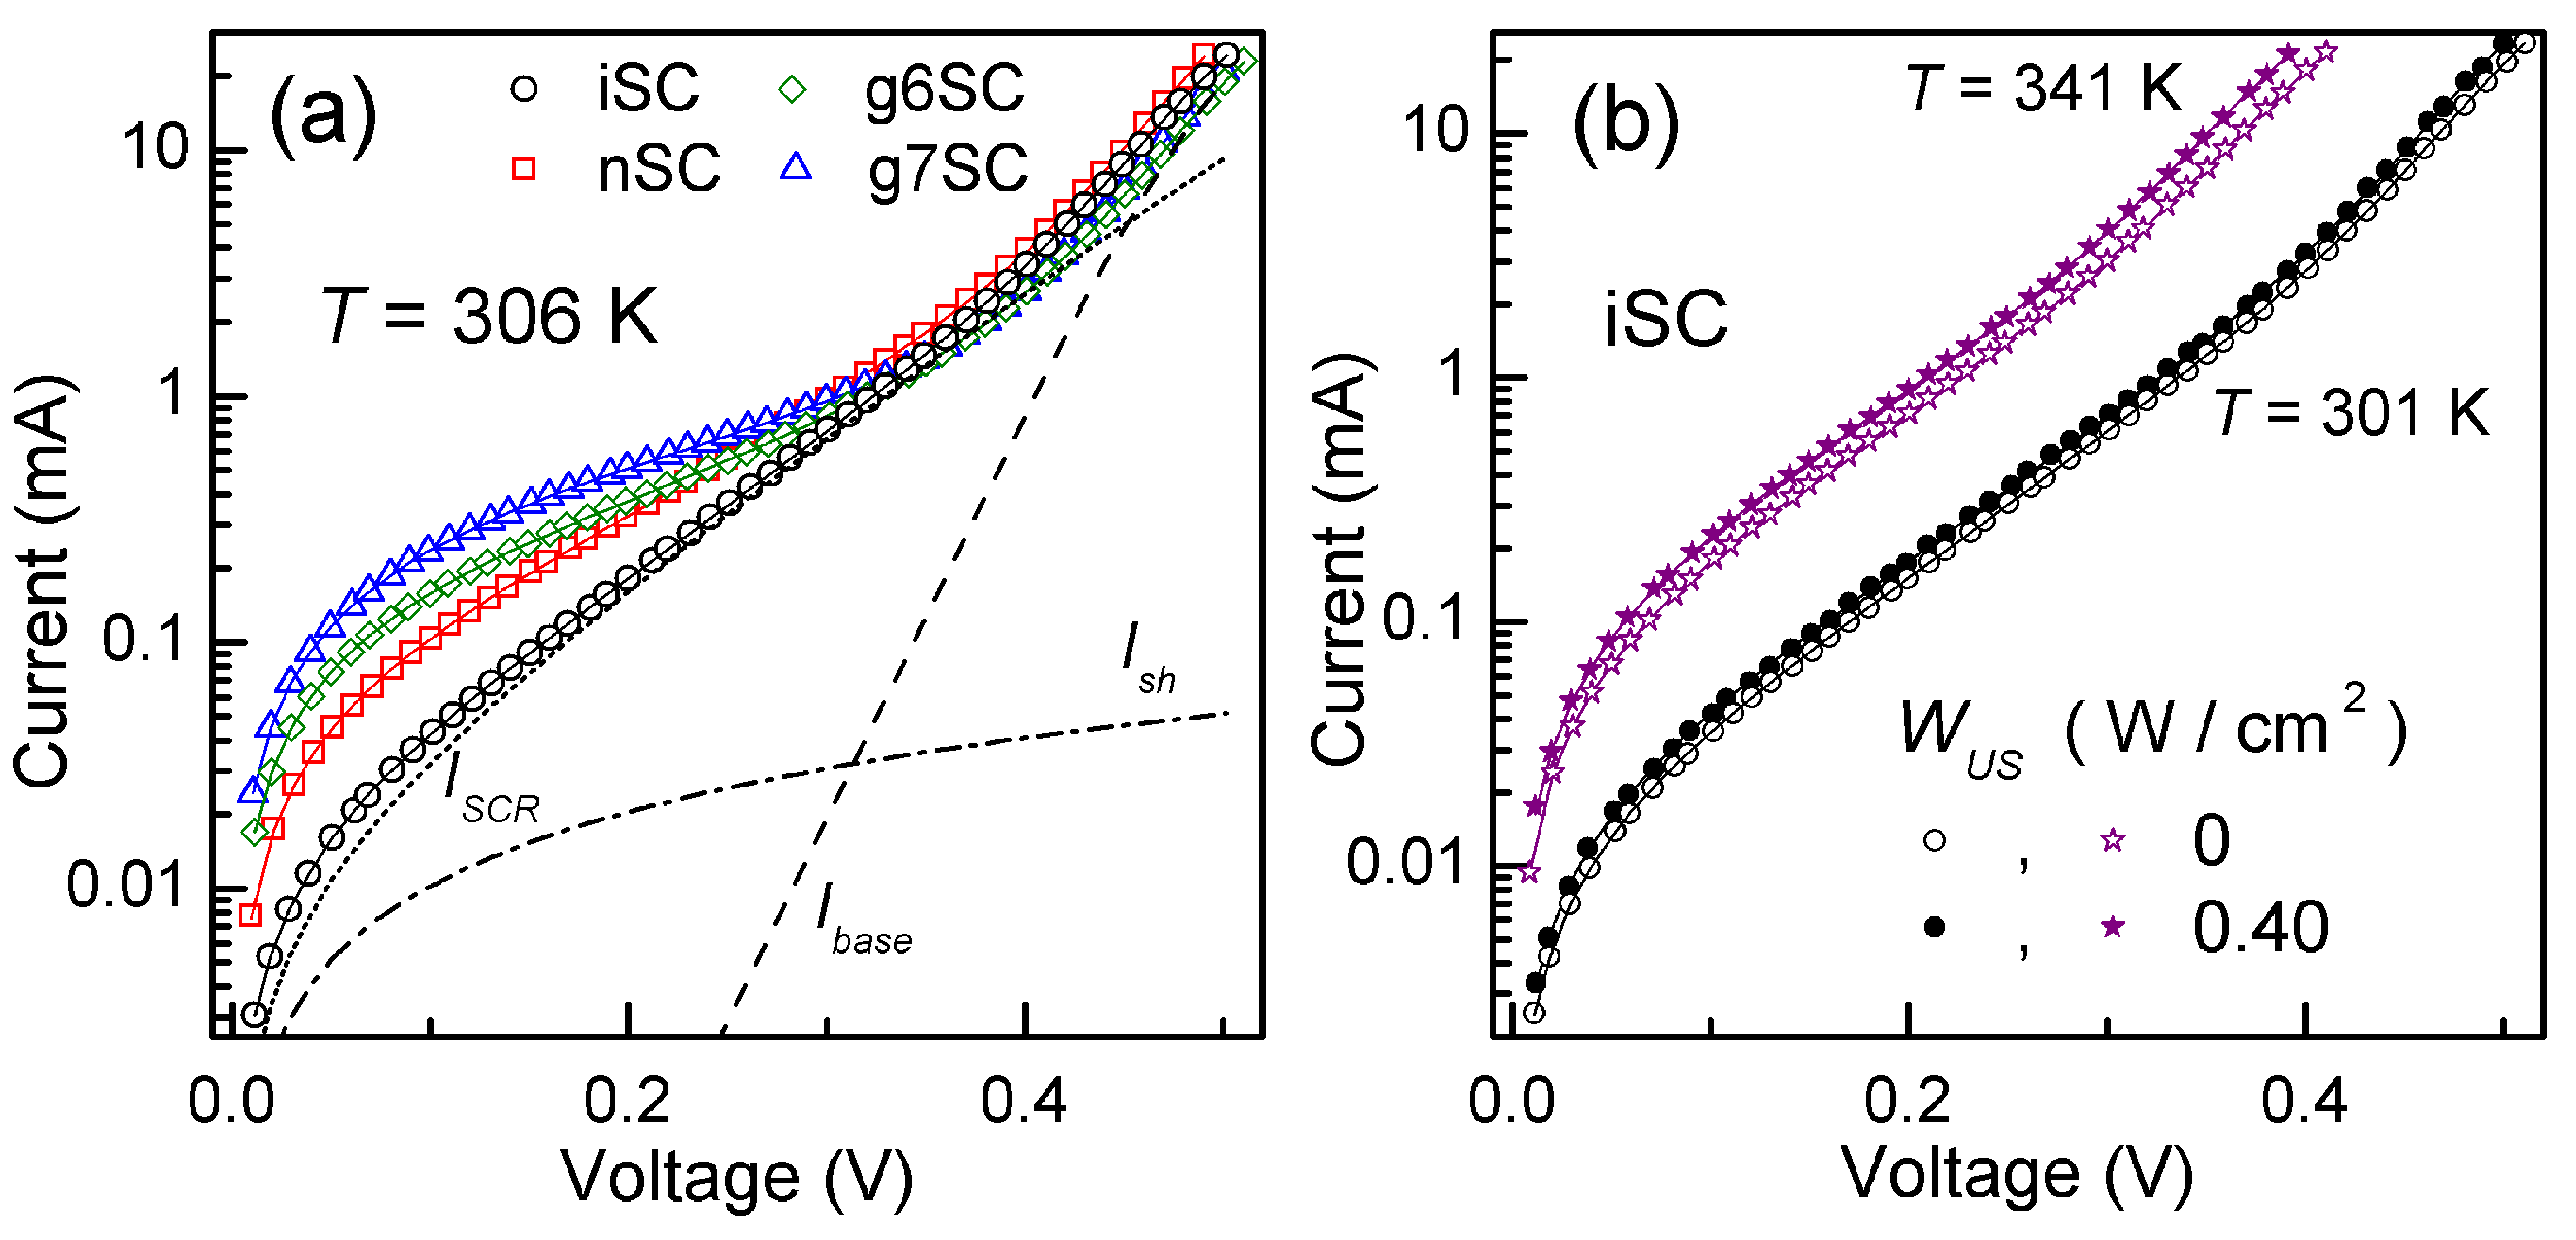
\includegraphics[width=0.7\textwidth]{fig_1ab}%
\caption{\label{figIV}
Dark $I$--$V$ characteristics measured (a) at 306~K for non--irradiated (circles), neutron--irradiated (squares) and gamma--irradiated (diamonds and triangles) structures without USL;
(b) at 301~K (circles) and 341~K (asterisks) with (filled marks, Ui--2) and without (open marks) USL for the iSC.
The marks are the experimental results, the solid lines are the fitted curves using Eqs.~(\ref{eqIV})--(\ref{eqW}).
The dashed, dotted and dot--dashed lines in (a) represent the calculated base, SCR and shunt components of full (black solid line) iSC current.
}%
\end{figure*}

The double--diode model of n$^+$--p structure $I$--$V$ characteristic is expressed in the following form:
\begin{eqnarray}
I(V,T)&=&I_{SCR}+I_{base}+I_{sh}\;,\label{eqIV}\\
I_{SCR}&=&\frac{qAn_id}{2\tau_{g}}\left\{\exp \left[\frac{q(V-IR_s)}{n_{\mathrm{id}}kT}\right]-1\right\}\,,\label{eqIscr}\\
I_{base}&=&\frac{qAn_i^2}{p_p}\sqrt{\frac{\mu_nkT}{\tau_n}}\left\{\exp \left[\frac{q(V-IR_s)}{kT}\right]-1\right\},\label{eqIbase}\\
I_{sh}&=&(V-IR_s)/R_{sh}\,,\label{eqIsh}
\end{eqnarray}
where
$I_{SCR}$ reflects the overall SCR recombination,
$I_{base}$ is closely related to recombination in the quasi-neutral region,
$I_{sh}$ is the shunt current,
$A$ is the sample area,
$n_i$ is the intrinsic carrier concentration,
$\tau_{g}$ is the SCR carrier lifetime,
$d$ is the  SCR thickness:
\begin{equation}
\label{eqW}
    d=\sqrt{\frac{2 \varepsilon \varepsilon_0}{q p_p}\left[
     \frac{E_g}{q}-\frac{kT}{q}\ln\!\left(\frac{N_vN_c}{p_pn_n}\right)-\frac{2kT}{q}-V\right]},
\end{equation}
$\varepsilon$ is the permittivity (11.7 for Si),
$p_p$ and $n_n$ are the majority carrier concentration in the $p$-- and $n$--type regions,
$E_g$ is the semiconductor band gap,
$N_c$ and $N_v$ are the effective density of states in the conduction and valence bands;
$n_{\mathrm{id}}$ is the ideality factor,
$R_s$ and $R_{sh}$ are the series and shunt resistances,
$\mu_n$ and $\tau_n$ are the electron (minority carrier) mobility and lifetime in the diode base.


We used Eqs. (\ref{eqIV})--(\ref{eqW}) to fit the experimental data and $\tau_g$, $\tau_n$, $n_{\mathrm{id}}$, $R_{sh}$, and $R_s$ were taken as the  fittings parameters.
The known \cite{ni:Green,Schroder2006,Markvart} temperature dependencies of $n_i$, $E_g$, and $\mu_n$ were used.
The extremely good fit to the experimental data was obtained --- see Fig.~\ref{figIV}.
In particular, the $R_s$ value about 1~$\Omega$ was determined for all samples.
Broken lines in Fig.~\ref{figIV}(a) demonstrate the example of calculated contributions of $I_{SCR}$, $I_{base}$, and $I_{sh}$ to full current.

In the USL case, the transverse AWs with frequency of $4.2$~MHz were exited with help of a piezoelectric transducer and were injected in samples from the base side in the [111]--direction.
The US intensities $W_{\mathtt{US}}$, amplitudes of lattice deformation $\xi_{\mathtt{US}}$ and lattice atom
displacement  $u_{\mathtt{US}}$ are listed in Table~\ref{tabUSL}.
It was reported previously \cite{Ostapenko1995,Olikh:Ultras,Ostrovskii2001} that the characteristic time of change in the silicon structure parameters under
the US action  did not exceed $2\cdot10^3$~s.
In order to wait till the AI transitional period the following experimental procedure has been used.
After USL start the sample has been kept at room temperature during 60~min and then the $I$--$V$ measurement and the sample heating were started.
In order to avoid the effect of piezoelectric field on $I$--$V$ characteristics, the piezoelectric transducer has been shielded.


\begin{table}
\caption{\label{tabUSL}The ultrasound loading parameters.
}
\begin{ruledtabular}
\begin{tabular}{ccccc}
Sample&$W_{\mathtt{US}}$ (W/cm$^2$)&$\xi_{\mathtt{US}}$ ($10^{-6}$)&$u_{\mathtt{US}}$ (nm)&USL label\\
\hline
iSC&0.22&3.1&0.67&Ui--1\\
&0.40&4.2&0.91&Ui--2\\
nSC&0.24&3.2&0.70&Un--1\\
&0.40&4.2&0.91&Un--2\\
g6SC&0.38&4.1&0.89&Ug6--2\\
g7SC&0.19&2.9&0.63&Ug7--1\\
&0.37&4.0&0.87&Ug7--2\\
\end{tabular}
\end{ruledtabular}
\end{table}

Fig.~\ref{fig_Reverse} illustrates the reversibility of AI effects.
The time interval between USL starting and "during" measurement was larger than 60~min,
the time interval between USL stopping and "after" measurement was about 24~h.
Data for nSC and g6SC are similar to those, which are presented for iSC and g7SC.

\begin{figure*}
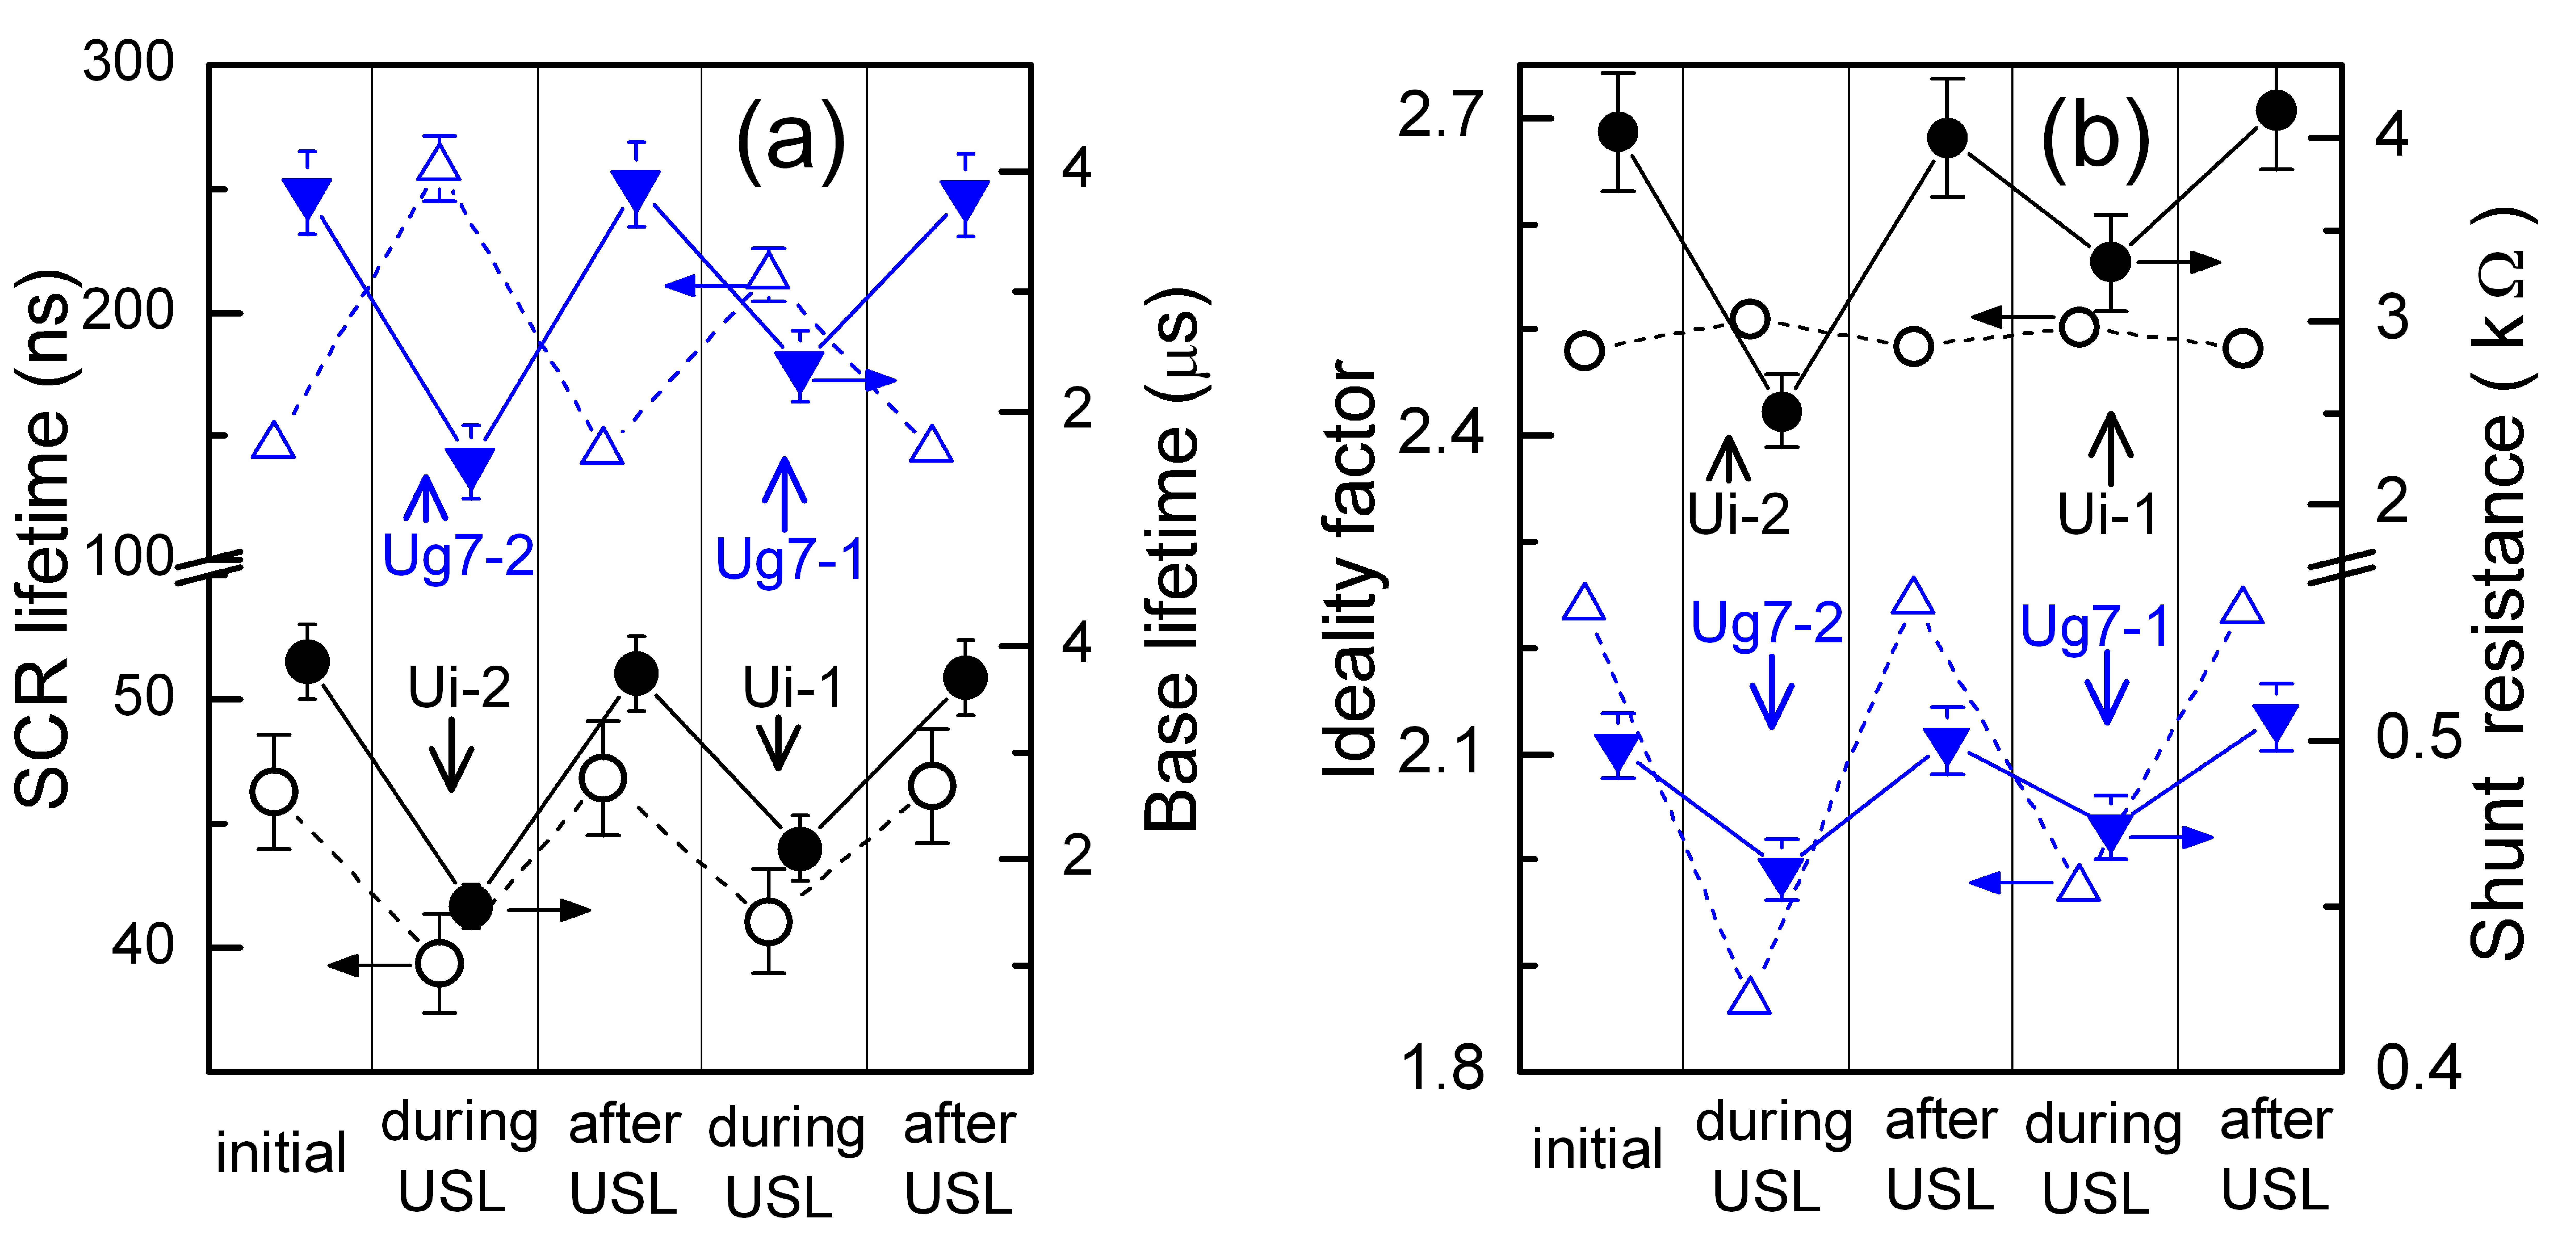
\includegraphics[width=0.7\textwidth]{fig_2ab}%
\caption{\label{fig_Reverse}
SCR lifetime (a, left axis, open marks),
base lifetime (a, right axis, filled marks),
ideality factor (b, left axis, open marks) and
shunt resistance (b, right axis, filled marks),
obtained before, during and after USL at 330~K.
Data for iSC (circles) and g7SC (triangles) are presented.
}%
\end{figure*}



The non-linear fittings were done by using the differential evolution method.\cite{DEWang}


\section{Results and Discussion}
\subsection{Space charge region\label{SCR}}
The $I$--$V$ characteristic parameters, which deal with SCR phenomena, are $n_{\mathrm{id}}$ and $\tau_{g}$.
The temperature dependences of ideality factor and SCR carrier lifetime are shown in Fig.~\ref{fig_n} and Fig.~\ref{fig_TAUg}, respectively.

\begin{figure*}
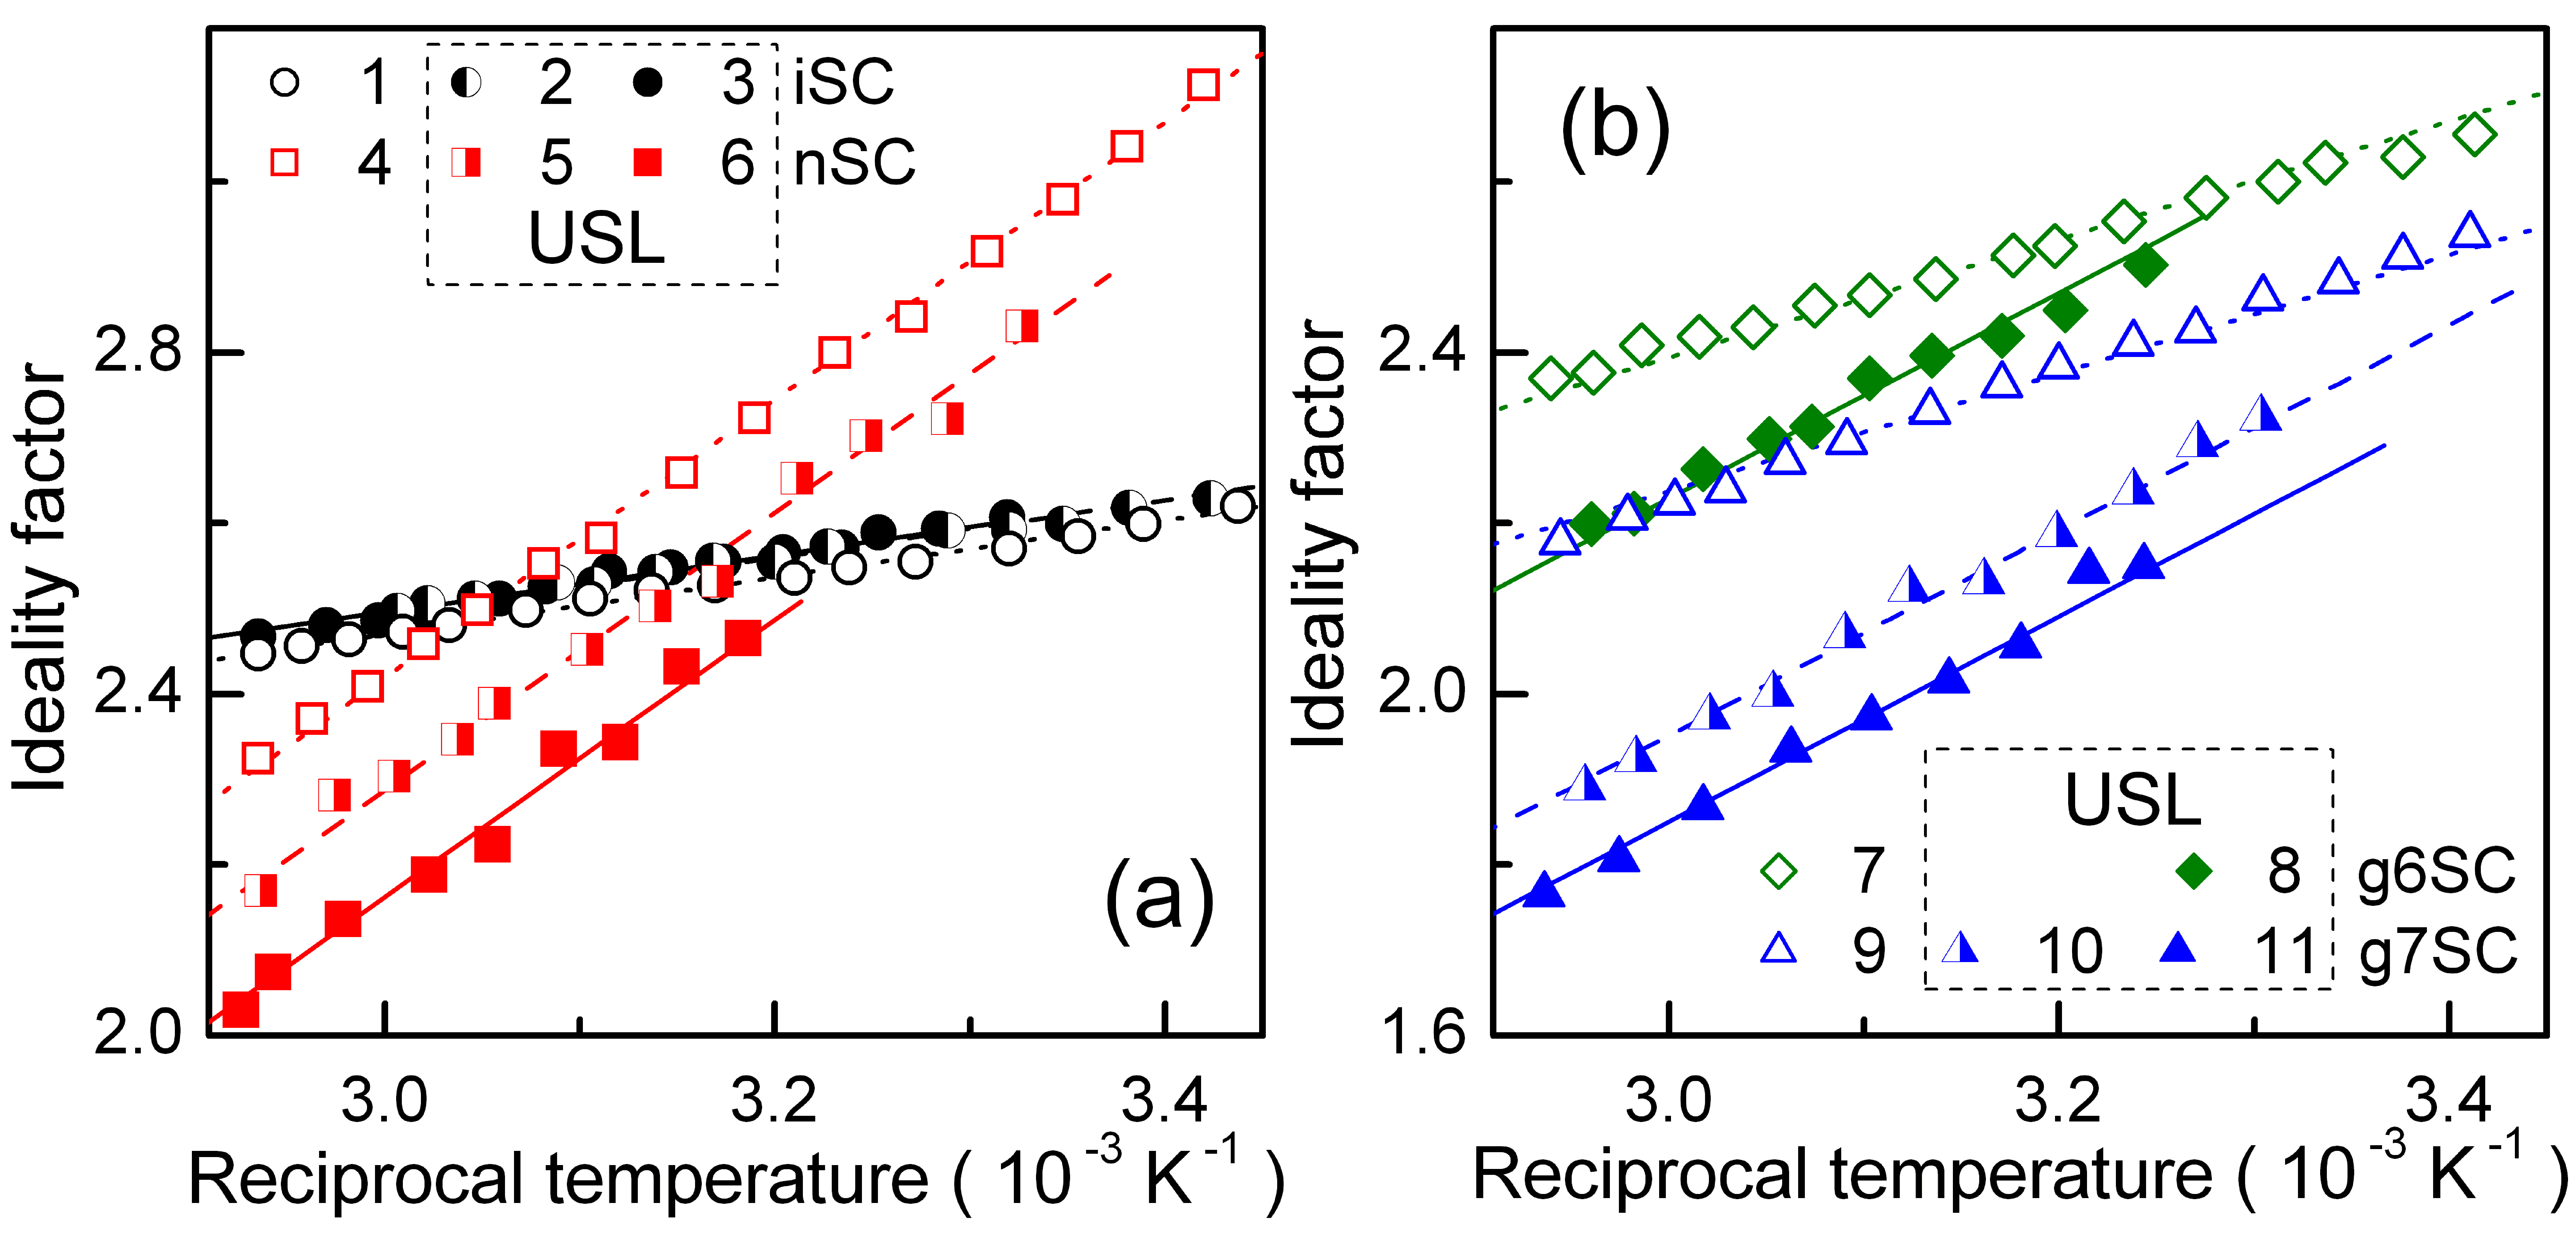
\includegraphics[width=0.7\textwidth]{fig_3ab}%
\caption{\label{fig_n}
Temperature dependences of ideality factor for non--irradiated (curves 1--3, circles),
neutron--irradiated (4--6, squares) and $\gamma$--irradiated (7--11, diamonds and triangles) samples.
The curves 1, 4, 7 and 9 (open marks) are obtained without USL,
curves 2, 3, 5, 6, 8, 10, and 11 correspond to
Ui--1, Ui--2, Un--1, Un--2, Ug6--2, Ug7--1, and Ug7--2 respectively.
The marks are the experimental results, the lines are the fitted curves using Eq.~(\ref{eq_nT}).
}%
\end{figure*}

\begin{figure*}
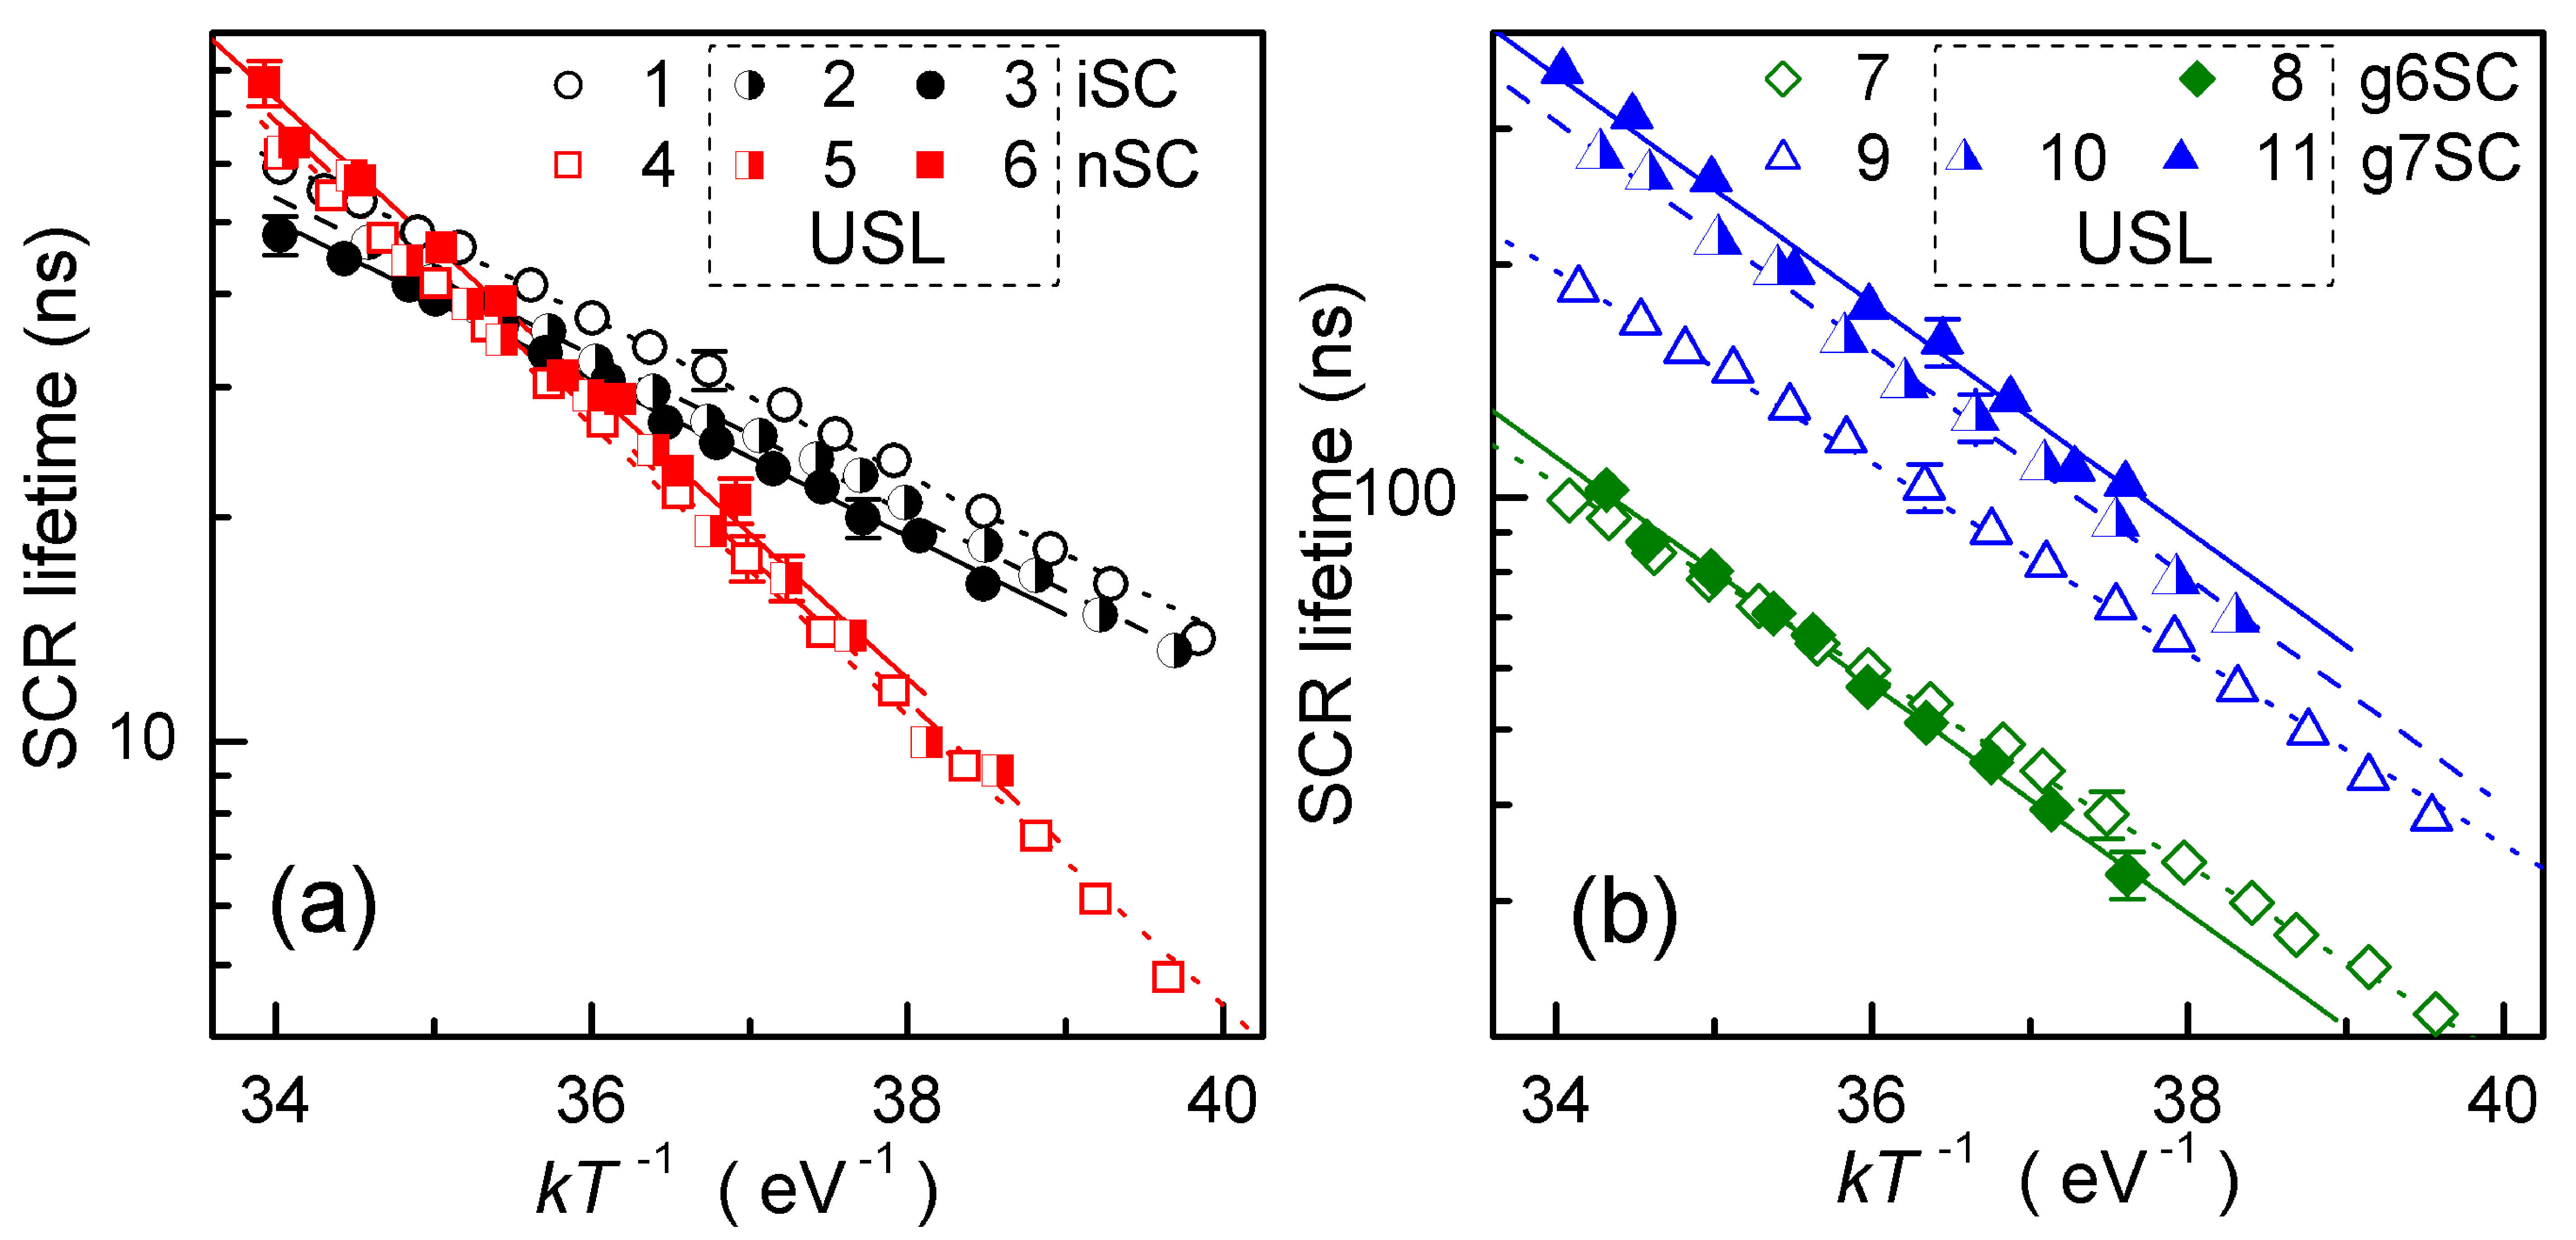
\includegraphics[width=0.7\textwidth]{fig_4ab}%
\caption{\label{fig_TAUg}
Temperature dependences of SCR lifetime for non--irradiated (curves 1--3, circles),
neutron--irradiated (4--6, squares) and $\gamma$--irradiated (7--11, diamonds and triangles) samples.
The curves 1, 4, 7 and 9 (open marks) are obtained without USL,
curves 2, 3, 5, 6, 8, 10, and 11 correspond to
Ui--1, Ui--2, Un--1, Un--2, Ug6--2, Ug7--1, and Ug7--2 respectively.
The marks are the experimental results, the lines are the fitted curves using Eq.~(\ref{eq_TAUgT}).
}%
\end{figure*}

As shown by the Fig.~\ref{fig_n} the ideality factor decreases with temperature increase and the plot $n_{\mathrm{id}}$ vs $1/T$  is close to linear.
Thus dependence $n_{\mathrm{id}}(T)$ can be expressed as
\begin{equation}
\label{eq_nT}
    n_{\mathrm{id}}(T)=n_{\mathrm{id},\infty}+T_{\mathrm{id}}/T\:.
\end{equation}
The thermoactivated growth of SCR lifetime is observed over the explored temperature range --- see Fig.~\ref{fig_TAUg}.
The temperature dependence of $\tau_{g}$ is sufficiently described by the equation
\begin{equation}
\label{eq_TAUgT}
    \tau_{g}(T)=\tau_{g0}\exp\left(-\frac{E_{\tau g}}{kT}\right)\:.
\end{equation}
The $T_{\mathrm{id}}$ and $E_{\tau g}$ values, determined for both non--irradiated and irradiated samples under USL as well as without it are listed in Table~\ref{tabTpar}.

\begin{table*}
\caption{\label{tabTpar}Characteristics of temperature dependences of $n^+$--$p$--Si structure parameters.
}
\begin{ruledtabular}
\begin{tabular}{cccccc}
Sample&USL&$T_{\mathrm{id}}$ (K)&$E_{\tau g}$ (eV)&$R_{293,\mathtt{Al}}$ (k$\Omega$)&$\sigma_{\mathtt{dis}}$ ($10^4$~K/$\Omega$)\\
\hline
iSC&non&$330\pm30$&$0.24\pm0.01$&$27\pm3$&$41\pm4$\\
&Ui--1&$310\pm30$&$0.24\pm0.01$&$27\pm3$&$50\pm4$\\
&Ui--2&$360\pm30$&$0.24\pm0.01$&$26\pm3$&$58\pm4$\\
nSC&non&$1610\pm70$&$0.45\pm0.02$&$2.2\pm0.4$&$65\pm7$\\
&Un--1&$1600\pm70$&$0.44\pm0.02$&$2.3\pm0.4$&$95\pm10$\\
&Un--2&$1680\pm70$&$0.44\pm0.02$&$2.2\pm0.4$&$130\pm10$\\
g6SC&non&$610\pm40$&$0.28\pm0.01$&$0.7\pm0.1$&$19\pm2$\\
&Ug6--2&$1080\pm50$&$0.33\pm0.02$&$0.8\pm0.1$&$24\pm2$\\
g7SC&non&$770\pm50$&$0.29\pm0.01$&$0.41\pm0.06$&$26\pm3$\\
&Ug7--1&$1260\pm60$&$0.34\pm0.02$&$0.39\pm0.06$&$45\pm4$\\
&Ug7--2&$1270\pm60$&$0.35\pm0.02$&$0.38\pm0.06$&$55\pm4$\\
\end{tabular}
\end{ruledtabular}
\end{table*}

We want to stress, that

\noindent
(i)~irradiation leads to $T_{\mathrm{id}}$ and $E_{\tau g}$ changes, the g6SC's characteristic temperature of ideality factor and SCR lifetime characteristic energy are closely related to those of g7SC under similar conditions;

\noindent
(ii)~USL affects $n_{\mathrm{id}}$ and $\tau_g$ values,
the absolute AI changes of ideality factor $\Delta n_{\mathrm{id}}=n_{\mathrm{id},\mathtt{US}}-n_{\mathrm{id},in}$ and
the relative AI changes of SCR lifetime $\varepsilon_{\tau g}=(\tau_{g,\mathtt{US}}-\tau_{g,in})/\tau_{g,in}$
(where subscripts ``$\mathtt{US}$'' and ``$in$'' identify the values,
obtained at the same temperature with and without USL respectively)
are listed in Table~\ref{tabAIchange};

\noindent
(iii)~$\Delta n_{\mathrm{id}}$ and $\varepsilon_{\tau g}$ vary with $W_{\mathtt{US}}$ enhancement, whereas $T_{\mathrm{id}}$ and $E_{\tau g}$ values practically do not depend on US intensity;


\noindent
(iv)~USL leads to increase  of both $T_{\mathrm{id}}$ and $E_{\tau g}$ in $\gamma$--irradiated samples (see Fig.~\ref{fig_n}(b) and Fig.~\ref{fig_TAUg}(b)),
but this effect is not observed in non--irradiated and neutron--irradiated samples (see Fig.~\ref{fig_n}(a) and Fig.~\ref{fig_TAUg}(a));

\noindent
(v)~$\Delta n_{\mathrm{id}}$ and $\varepsilon_{\tau g}$ have an opposite sign for non--irradiated and irradiated samples
(for SCg6 not in whole temperature range);

\noindent
(vi)~ideality factor is varied by USL more effectively in irradiated samples;


\begin{table}
\caption{\label{tabAIchange}Acoustically induced change of $n^+$-$p$--Si structure parameters (at 330~K).
}
\begin{ruledtabular}
\begin{tabular}{cccccc}
Sample&USL&$\Delta n_{\mathrm{id}}$ &$\varepsilon_{\tau g}$ &$\varepsilon_{\tau n}$ &$\varepsilon_{\sigma\mathtt{dis}}$ \\
&&\mbox{($\pm0.01$)}&($\pm5$\%)&($\pm0.2$)&($\pm10$\%)\\
\hline
iSC&Ui--1&0.02&-14&0.7&20\\
&Ui--2&0.03&-17&1.4&40\\
nSC&Un--1&-0.13&5&1.5&50\\
&Un--2&-0.26&13&3.0&100\\
g6SC&Ug6--2&-0.15&2&2.3&30\\
g7SC&Ug7--1&-0.26&49&0.9&70\\
&Ug7--2&-0.36&70&1.9&110\\
\end{tabular}
\end{ruledtabular}
\end{table}


For the purpose of present consideration, it is important to discuss the recombination mechanism in the SCR of the investigated samples.
According to classical SRH theory, an ideality factor must be less than 2 and
$\tau_g$ temperature dependence is expected \cite{TAUg:Schroder,TAUg:Aharoni} to be described by the relation  $\tau_g\simeq2\,\tau_n\sqrt{\sigma_n/\sigma_p}\cosh\left[\left(E_t-E_i\right)/kT\right]$
(where $\sigma_n$, $\sigma_p$, and  $E_t$ are the electron and hole capture cross sections (CCSs) and the energy  level of  the  recombination  center,
$E_i$  is the  intrinsic  energy level).
In our case, $n_{\mathrm{id}}$ is lager than 2 and $\tau_g$ increases with temperature.
Therefore SRH theory is inapplicable to the investigated samples.
Several attempts to explain large $n_{\mathrm{id}}$ value have been made with various models.\cite{Heide,Beier,Shah,Kaminski_n}
But all observed features of SCR recombination (ideality factor large value, independence on light intensity, dependence on temperature
as well as carrier lifetime small value) can be explained by the model of coupled defect level recombination (CDLR) \cite{CDLR:JAP1995,CDLR:JAP} only.
This model provides a rapid  direct  charge  transfer  between  defect levels.
Such phenomenon has been observed experimentally firstly \cite{DAPR:Chen1991,DAPR:Chen1994} and then it was recruited to explain process in semiconductor diodes. \cite{CDLR:JAP1995,CDLR:JAP,CDLR:SSP}

According to the CDLR model, recombination is the result of carrier exchange between two defect level and crystal bands.
In particular, it is proposed \cite{CDLR:JAP} that the recombination rate is dominated by sites where acceptor--like defect is coupled with donor-like defect.
In simplified case of
no carrier exchange between the donor level $E_t^{\mathtt{D}}$ and the valence band
as well as between the acceptor level $E_t^{\mathtt{A}}$ and the conduction band,
the recombination rate $R$ can be expressed\cite{CDLR:JAP1995} as
\begin{eqnarray}
R&=&\frac{R_{12}-\sqrt{R_{12}^{\,2}-4\tau_{n}^{\mathtt{D}}\tau_{p}^{\mathtt{A}}(np-n_i^2)(1-\epsilon)}}{2\tau_{n}^{\mathtt{D}}\tau_{p}^{\mathtt{A}}(1-\epsilon)}\;,\label{eqR}\\
R_{12}&=&\frac{(n+n_{\mathtt{D}})(p+p_{\mathtt{A}})}{R_{\mathtt{DA}}}+
\tau_{n}^{\mathtt{D}}(p+p_{\mathtt{D}})+\tau_{p}^{\mathtt{A}}(n+n_{\mathtt{A}}),\label{eqR12}\\
\tau_{n}^{\mathtt{D}}&=&(N_{\mathtt{D}}\,\sigma_{n}^{\mathtt{D}}\,\upsilon_{\mathrm{th},n})^{-1},\,\,\,\,
\tau_{p}^{\mathtt{A}}=(N_{\mathtt{A}}\,\sigma_{p}^{\mathtt{A}}\,\upsilon_{\mathrm{th},p})^{-1},\label{eqTAU}
\end{eqnarray}
where
$R_{\mathtt{DA}}$ is the coupling parameter,
$N_{\mathtt{D}}$ and $N_{\mathtt{A}}$ are the densities of donor and acceptor--like defects,
$\sigma_{n}^{\mathtt{D}}$ and $\sigma_{p}^{\mathtt{A}}$ are electron CCS of donor and hole CCS of acceptor,
$\upsilon_{\mathrm{th},n}$ and $\upsilon_{\mathrm{th},p}$ are the thermal electron and hole velocities,
$n_{\mathtt{D,A}}$, $p_{\,\mathtt{D,A}}$, and $\epsilon$ depend on $E_t^{\mathtt{D}}$, $E_t^{\mathtt{A}}$, and level degeneracy  factors.
As $\tau_g\propto R^{-1}$, the last three values are expected to provide a thermoactivated behavior of SCR lifetime.
Unfortunately, the equation does not account for the functional relation between $I$--$V$ characteristic parameters and attributes of defects, taking part in CDLR.

According to Steingrube \emph{et al}.\cite{CDLR:JAP},
SSC for defect in a pair differs from that for isolated defect and depends on the distance between donor and acceptor $r$:
\begin{equation}
\label{eqSigma}
\sigma_{n,p}^{\mathtt{D,A}}(r)=C_{n,p}^{\mathtt{D,A}}\,r^2\,,
\end{equation}
where $C_{n}^{\mathtt{D}}$ and $C_{p}^{\mathtt{A}}$ are constant values.
Besides, $R_{\mathtt{DA}}$ is proportional to the overlap integral of the defects wave functions.
If both defects are characterized by H--like radial--symmetric wave function and equal Bohr radius $a_0$,
the following expression can be used: \cite{CDLR:JAP}
\begin{equation}
\label{eqRda}
R_{\mathtt{DA}} (r) \propto N_{\mathtt{D}}N_{\mathtt{A}}\left[1+\frac{r}{a_0}+\frac{1}{3}\left(\frac{r}{a_0}\right)^2\right]
   e^{-r/a_0}\,.
\end{equation}


In our opinion, the observed reversible AI $n_{\mathrm{id}}$ and $\tau_g$ modifications are induced by
donor--acceptor distance alteration in samples under USL.
Really, according to data,\cite{MirzadeJAP2011,PeleshchakUJF2016} the force acting on the point defect during USL can be expressed as
\begin{equation}
\label{eqFd}
F_d=\chi\,\Delta\Omega_d\frac{\partial \xi(z,t)}{\partial z}\,,
\end{equation}
where
$\chi$ is the bulk elasticity modulus,
$\Delta\Omega_d$ is the crystal volume change per defect,
$\xi$ is the crystal lattice deformation,
and AW propagates along $z$ axis,
$\partial \xi(z,t)/\partial z\propto \xi_{\mathtt{US}}$.
For interstitial atoms and substitutional impurities with ionic radius exceeding the ionic radius of matrix
atoms, the $\Delta\Omega_d > 0$, whereas,
for vacancies and substitutional impurities with ionic radius smaller than the ionic radius of matrix atoms,
$\Delta\Omega_d < 0$.
Therefore, a point defect vibrates under USL and oscillation amplitude and phase are determined by both the defect character and the intensity of AW.

\begin{figure}
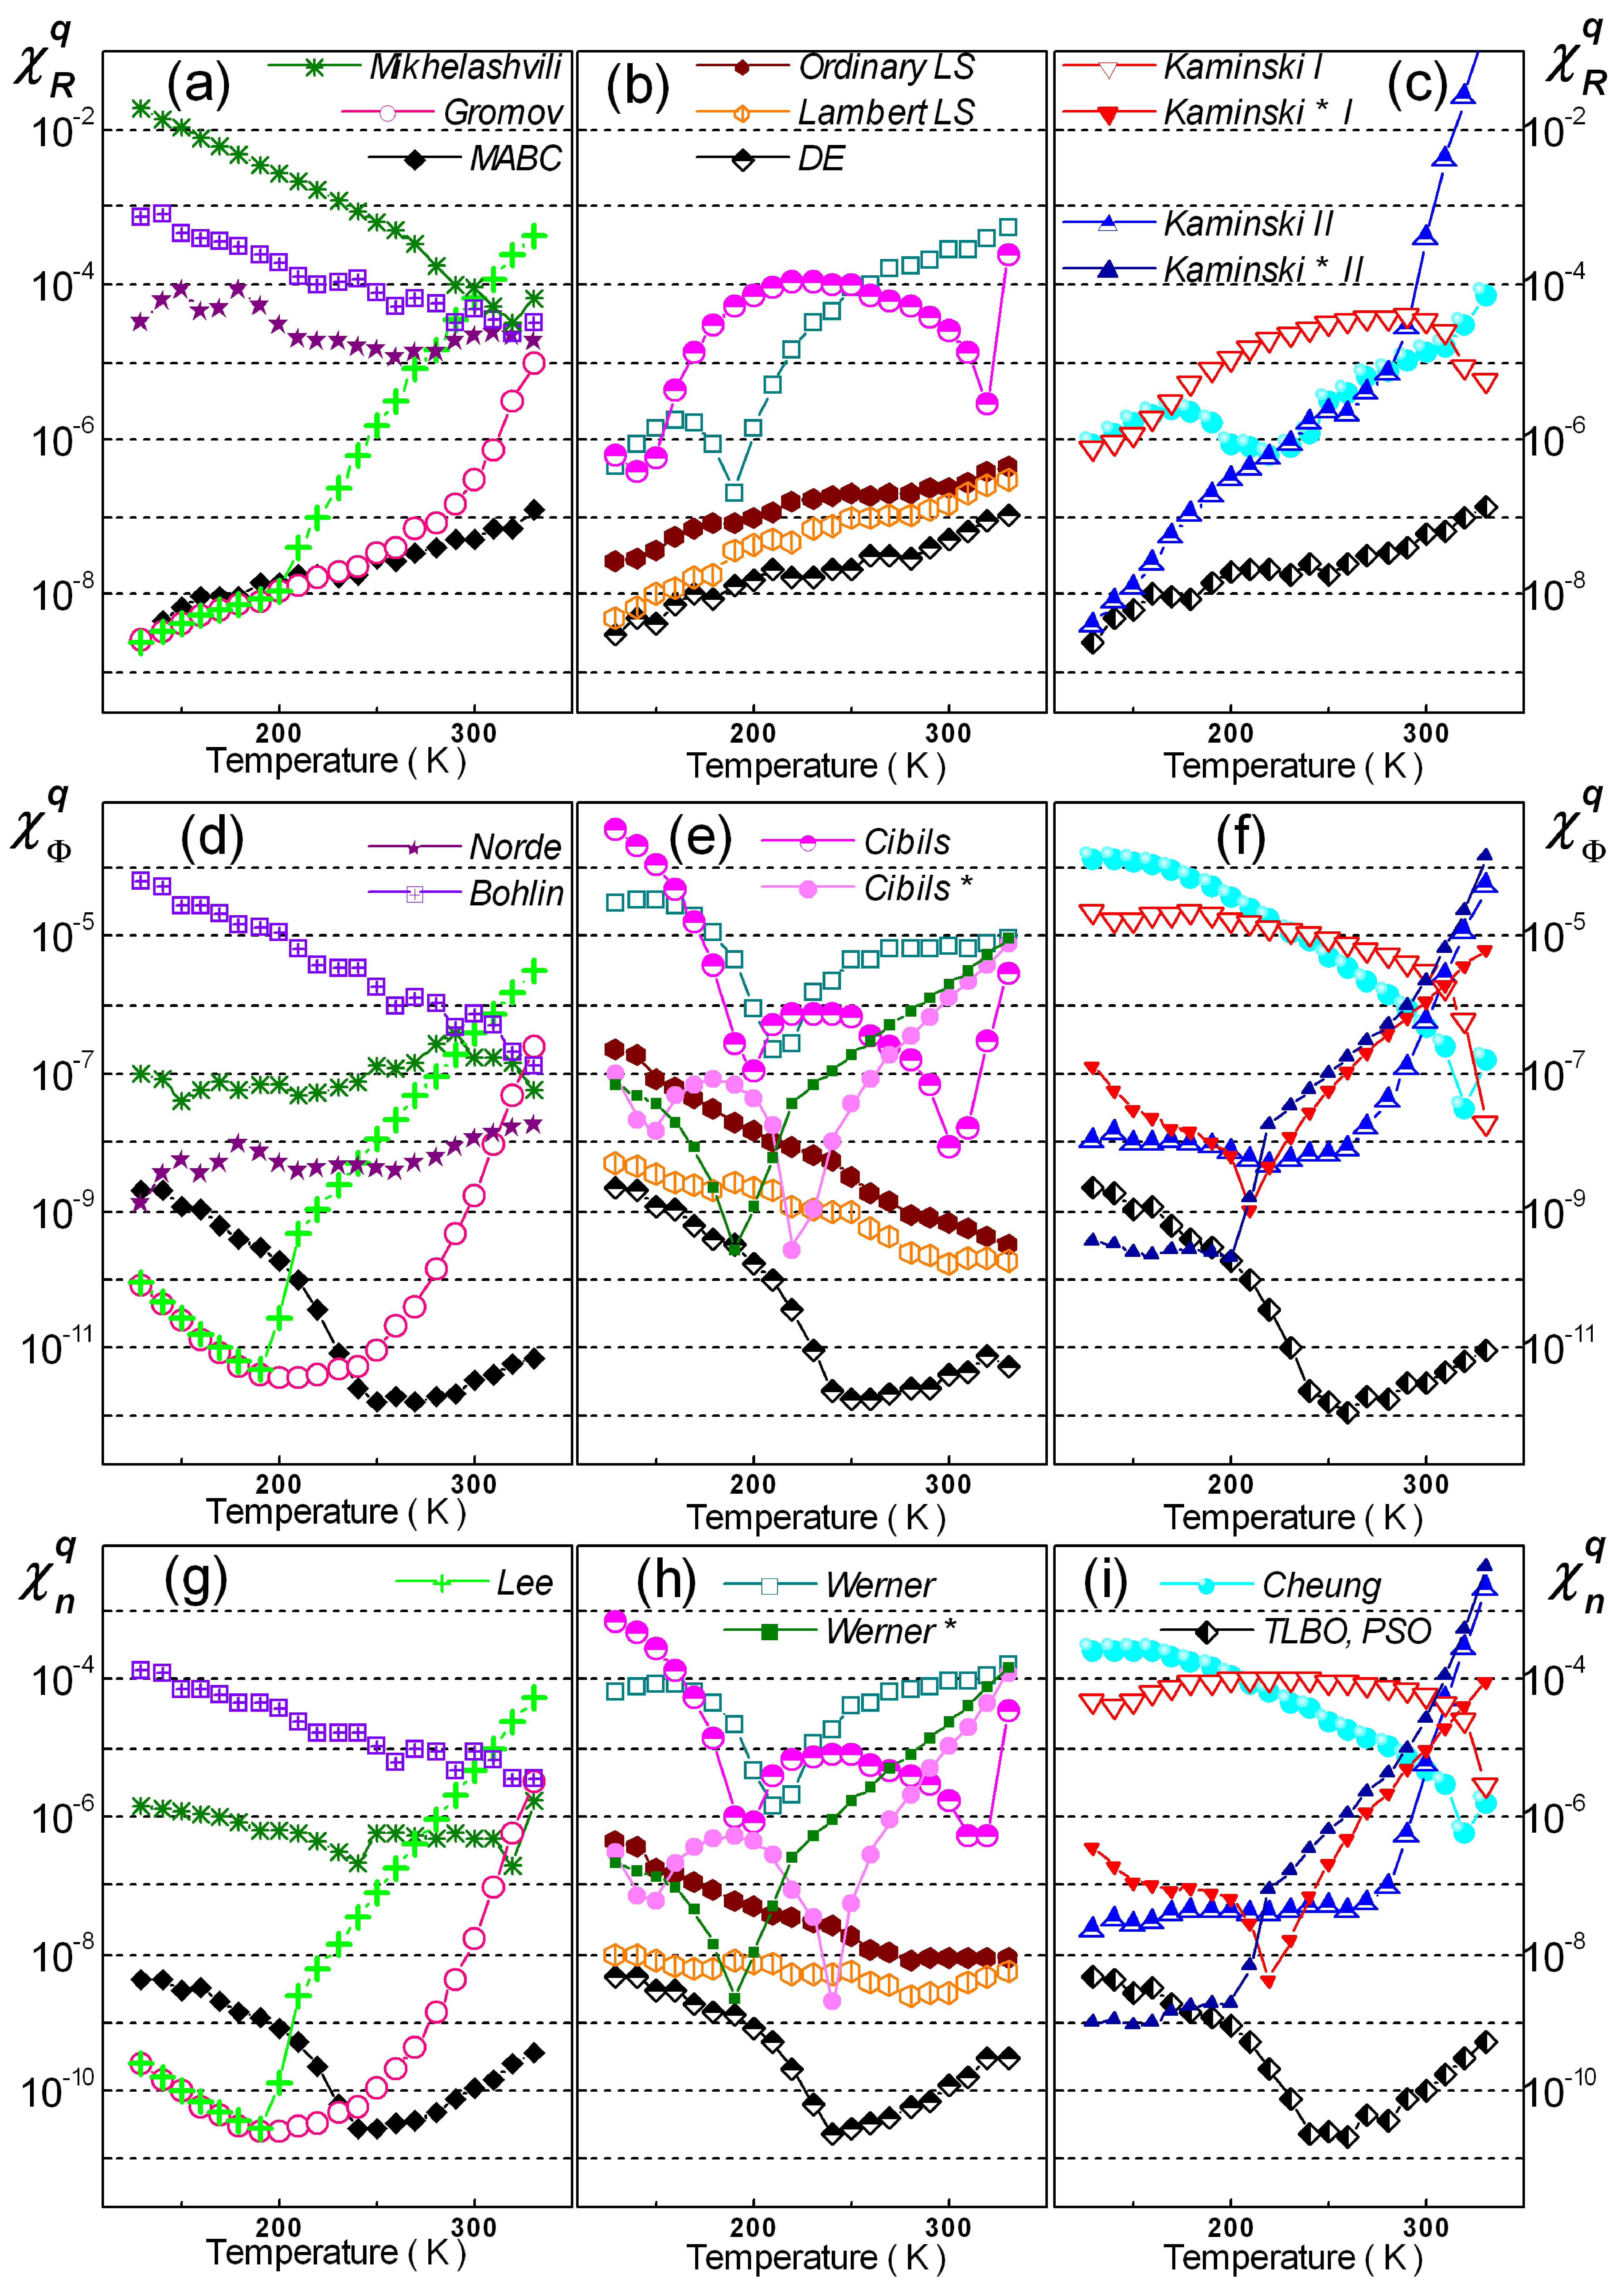
\includegraphics[width=0.45\textwidth]{fig_5}%
\caption{\label{fig_Model}
Model of CDLR center behavior under US action.
}%
\end{figure}

The simplest model, which is shown in Fig.~\ref{fig_Model}, gives the following  qualitative conclusion.
Initially donor and acceptor are separated by the distance $r_{in}$.
Axis X is drawn through point defect initial positions.
Under USL defects would vibrate with amplitudes $u_\mathtt{D}$ and $u_\mathtt{A}$.
Vibration axis coincides with AW displacement direction and forms angle $\varphi$ with  X--axis.
The defect vibration amplitudes depend on $\xi_{U\!S}$, defect elastic strain ($\Delta\Omega_d^\mathtt{D}$ and $\Delta\Omega_d^\mathtt{A}$), defect coupling  and may have different values.
According to suggested model, the donor--acceptor distance in the sample under USL $r_\mathtt{US}$ depends on time $t$:
\begin{multline}
\label{eqrUS}
r_\mathtt{US}(t)=\left\{[r_{in}+u_\mathtt{A}\cos(\omega_\mathtt{US}t+\delta)-u_\mathtt{D}\cos(\omega_\mathtt{US}t)]^2\cos^2\varphi \right.\\
    \left.+ [u_\mathtt{A}\cos(\omega_\mathtt{US}t+\delta)-u_\mathtt{D}\cos(\omega_\mathtt{US}t)]^2\sin^2\varphi\right\}^{0.5}\,,
\end{multline}
where $\omega_\mathtt{US}$ is the US cyclic frequency,
$\delta$ is the phase shift between donor and acceptor vibration.

We use Eqs.~(\ref{eqSigma})--(\ref{eqRda}) to estimate AI relative changes of CCS
$\varepsilon_\sigma=[\sigma_{\mathtt{US}}-\sigma(r_{in})]/\sigma(r_{in})$
and coupling parameters $\varepsilon_{\mathtt{RDA}}=[R_{\mathtt{DA,US}}-R_\mathtt{DA}(r_{in})]/R_\mathtt{DA}(r_{in})$,
where $\sigma_{\mathtt{US}}$ and $R_{\mathtt{DA,US}}$ are averaged over the AW period $T_\mathtt{US}$:
\begin{equation*}
\label{eqAver}
\sigma_{\mathtt{US}}=\frac{1}{T_\mathtt{US}}\int^{T_\mathtt{US}}_0\!\!\!\!\!\!\sigma(r_\mathtt{US}(t))dt\,,
R_{\mathtt{DA,US}}=\frac{1}{T_\mathtt{US}}\int^{T_\mathtt{US}}_0\!\!\!\!\!\!R_{\mathtt{DA}}(r_\mathtt{US}(t))dt\,.
\end{equation*}
In this estimation, the relaxation time in the CDLR sub--system is assumed to be considerably less than $T_\mathtt{US}$
and the previously used\cite{CDLR:JAP} value $a_0=3.23$~nm is applied.
Besides, the chosen $u_\mathtt{D}$ and $u_\mathtt{A}$ values are commensurate with $u_\mathtt{US}$.
But it is taken into account, that a displacement of the point defect without covalent bond could exceed a matrix atom displacement.
At last, no US  absorption by defect is assumed.
In this simple case $\delta$ equals to $0^\circ$, if $(\Delta\Omega_d^\mathtt{D}\cdot\Delta\Omega_d^\mathtt{A})>0$,
or to $180^\circ$, if $(\Delta\Omega_d^\mathtt{D}\cdot\Delta\Omega_d^\mathtt{A})<0$.
In addition, $\varepsilon_{\mathtt{RDA}}$ dependence on
$u_\mathtt{D}$ and $u_\mathtt{A}$
is only determined by $|u_\mathtt{D}-u_\mathtt{A}|$ ($\delta=0^\circ$ case) or $|u_\mathtt{D}+u_\mathtt{A}|$ ($\delta=180^\circ$ case).
Moreover, these dependences are identical in both cases.
The typical results of simulation of coupling parameter changes are shown in  Fig.~\ref{fig_Erda}.


\begin{figure}
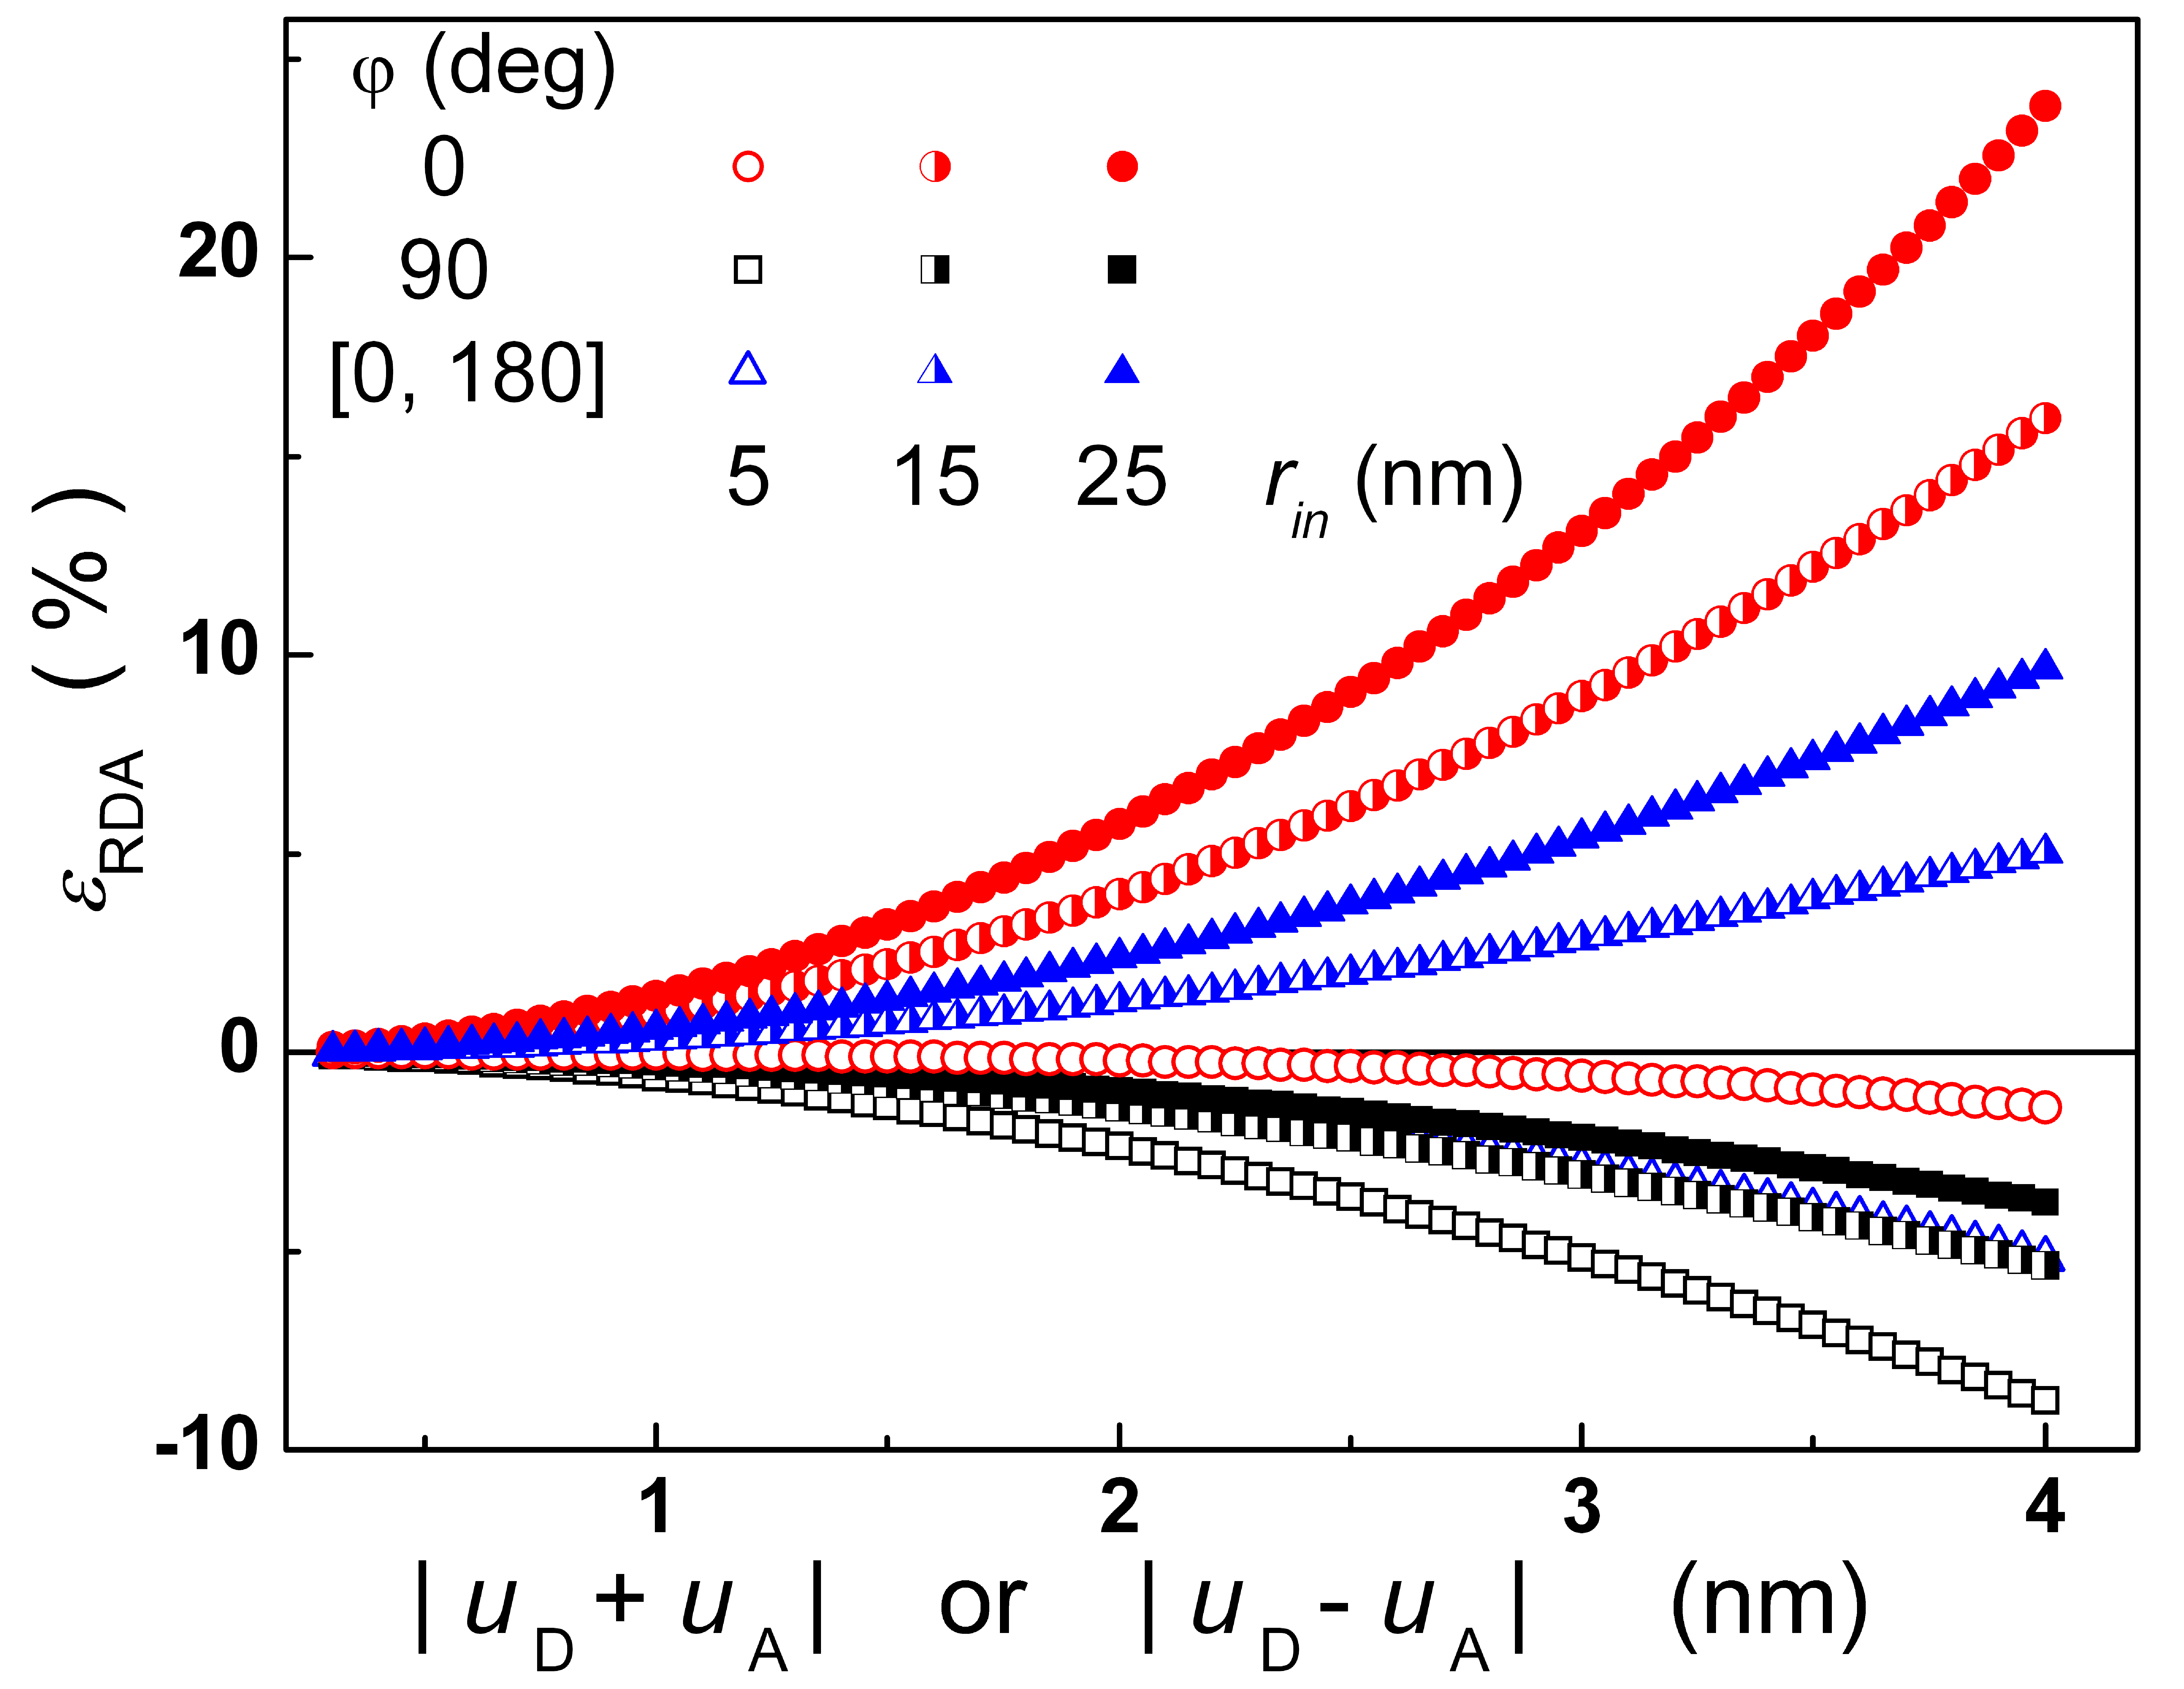
\includegraphics[width=0.45\textwidth]{fig_6}%
\caption{\label{fig_Erda}
Simulated dependencies of AI changes of coupling parameter on the vibration amplitudes.
Axis $|u_\mathtt{D}-u_\mathtt{A}|$ corresponds to $\delta=0^\circ$ case, whereas axis $|u_\mathtt{D}+u_\mathtt{A}|$ corresponds to $\delta=180^\circ$ case.
The parameters are set to $a_0=3.23$~nm,
$r_{in}=5$~nm (open marks), $15$~nm (semi--filled marks), and $25$~nm (filled marks),
$\varphi=0^\circ$ (circles), $90^\circ$ (squares).
Triangles correspond to mean $\varepsilon_{\mathtt{RDA}}$ value for $[0^\circ\div 180^\circ]$ $\varphi$ range.
}%
\end{figure}

$\varepsilon_{\sigma}$ depends on oscillation amplitudes with a similar features and
does not depend on $\varphi$:
\begin{equation}
\label{eqEpsSig}
\varepsilon_{\sigma}=(u_\mathtt{D}\pm u_\mathtt{A})^2/2\,r_{in}^2=K_\mathtt{US}^\mathtt{DA}W_{\mathtt{US}}\,,
\end{equation}
where``$+$'' and ``$-$'' correspond to $\delta=180^\circ$ and $\delta=0^\circ$ respectively,
$K_\mathtt{US}^\mathtt{DA}$ characterizes defect couple--ultrasound interaction and depends on properties defects as well as crystal matrix.
It is taken into account in Eq.~(\ref{eqEpsSig}), that $u_\mathtt{D},u_\mathtt{A}\propto \xi_\mathtt{US}\propto\sqrt{W_\mathtt{US}}$.

It is worth keeping in mind, that
CLDR current flows locally in the locations of extended defects.\cite{CDLR:JAP,CDLR:SSP}
On the other hand, dislocations are often situated in the SCR region perpendicularly to $p-n$ junction plane
and investigated samples are not exception (see Section~\ref{Rsh}).
If CDLR in the dislocation locations is assumed, then dislocations with edge component would affect the pair spatial orientation.
Thus axis of donor--acceptor pair with $(\Delta\Omega_d^\mathtt{D}\cdot\Delta\Omega_d^\mathtt{A}>0)$  should be predominantly parallel to dislocation line,
whereas the axis of the pair of coupled defects with $(\Delta\Omega_d^\mathtt{D}\cdot\Delta\Omega_d^\mathtt{A}<0)$ should make a right angle with it.
As AW displacement is parallel to the $p-n$ junction plane,
the cases of most exciting interest are following:

\noindent  $\delta=0^\circ$, $\varphi=90^\circ$ ($\Delta\Omega_d^\mathtt{D}\cdot\Delta\Omega_d^\mathtt{A}>0$ case);

\noindent  $\delta=180^\circ$, $\varphi\in[0^\circ\div 180^\circ]$ ($\Delta\Omega_d^\mathtt{D}\cdot\Delta\Omega_d^\mathtt{A}<0$ case).

\noindent
In other words, all curves in Fig.~\ref{fig_Erda} can be realized if defect volume relaxation of donor--like defect has the sign opposite to that of acceptor--like defect.
And only squares have to be under consideration in $\Delta\Omega_d^\mathtt{D}\cdot\Delta\Omega_d^\mathtt{A}>0$ case.

Taking into account the experimental results and suggested model estimation:

\noindent
(i)~$E_{\tau g}$ and $T_{\mathrm{id}}$ are mainly determined by couple component energy levels.
The alteration of $E_{\tau g}$ and $T_{\mathrm{id}}$ for nSC, g6SC, and g7SC in comparison with iSC testifies on the change of defect (donor, acceptor, or both),
which take part in CDLR, after irradiation.
And g6SC defect is coincident to g7SC defect and differs from neutron--irradiated sample defect.

\noindent
(ii)~USL causes donor--acceptor distance change and results in $\varepsilon_{\sigma}$ and $\varepsilon_{\mathtt{RDA}}$,
which increase with $W_{\mathtt{US}}$.

\noindent
(iii)~Acoustically induced $E_{\tau g}$ (and $T_{\mathrm{id}}$) modification, which is observed in g6SC, and g7SC only,
testifies on the rebuilding of  $\gamma$--induced RD.
I.e., $\gamma$--induced RD is configurationally bistable (or metastable) and transforms from ground state to another under US action.
Similar AI defect variations were also reported previously.\cite{Wosinski,Ostapenko1994,Olikh2009Sem,YOlikhTPL2011}

\noindent
(iv)~$\varepsilon_{\sigma}$ sign is immutable --- see Eq.~(\ref{eqEpsSig}),
whereas $\varepsilon_{\mathtt{RDA}}$ sign can vary for a pair with opposite relaxation volume component (see Fig.~\ref{fig_Erda}).
Therefore $\Delta n_{\mathrm{id}}$ and $\varepsilon_{\tau g}$ sign change is an evidence of transformation
from $(\Delta\Omega_d^\mathtt{D}\cdot\Delta\Omega_d^\mathtt{A}>0)$  to
$(\Delta\Omega_d^\mathtt{D}\cdot\Delta\Omega_d^\mathtt{A}<0)$  after irradiation.
Transformation is confirmed by rise of US influence efficiency in irradiated samples.
Really, in the case of $(\Delta\Omega_d^\mathtt{D}\cdot\Delta\Omega_d^\mathtt{A}<0)$ the US efficiency is determined by the sum of pair component displacements,
whereas in the contrary case  --- by their difference.
Conceivably, both donor and acceptor are of interstitial--type in non--irradiated sample, and one of pair component is of vacancy--type in irradiated samples.
The defect configuration are discussed below, in Section~\ref{DefectType}.


\subsection{Quasi--neutral region\label{Base}}

Base lifetime mirrors the processes, which occur in the quasi--neutral region  of $p$-$n$--structure.
Fig.~\ref{fig_TAUr} shows the  $\tau_n$  behaviour in the explored temperature range.
Minority carrier lifetime expectedly rises with temperature increase and
$\tau_n$ values equal to $2\div5$~$\mu$s for different samples at 320~K.
These values correspond to $80\div130$~$\mu$m range of diffusion length.
In our opinion, the observed $\tau_n$ dispersion is not defined by irradiation, but deals with sample--ancestor wafer inhomogeneity, which is revealed
quite often.\cite{Oxide:Chen,Oxide_Schon}

\begin{figure*}
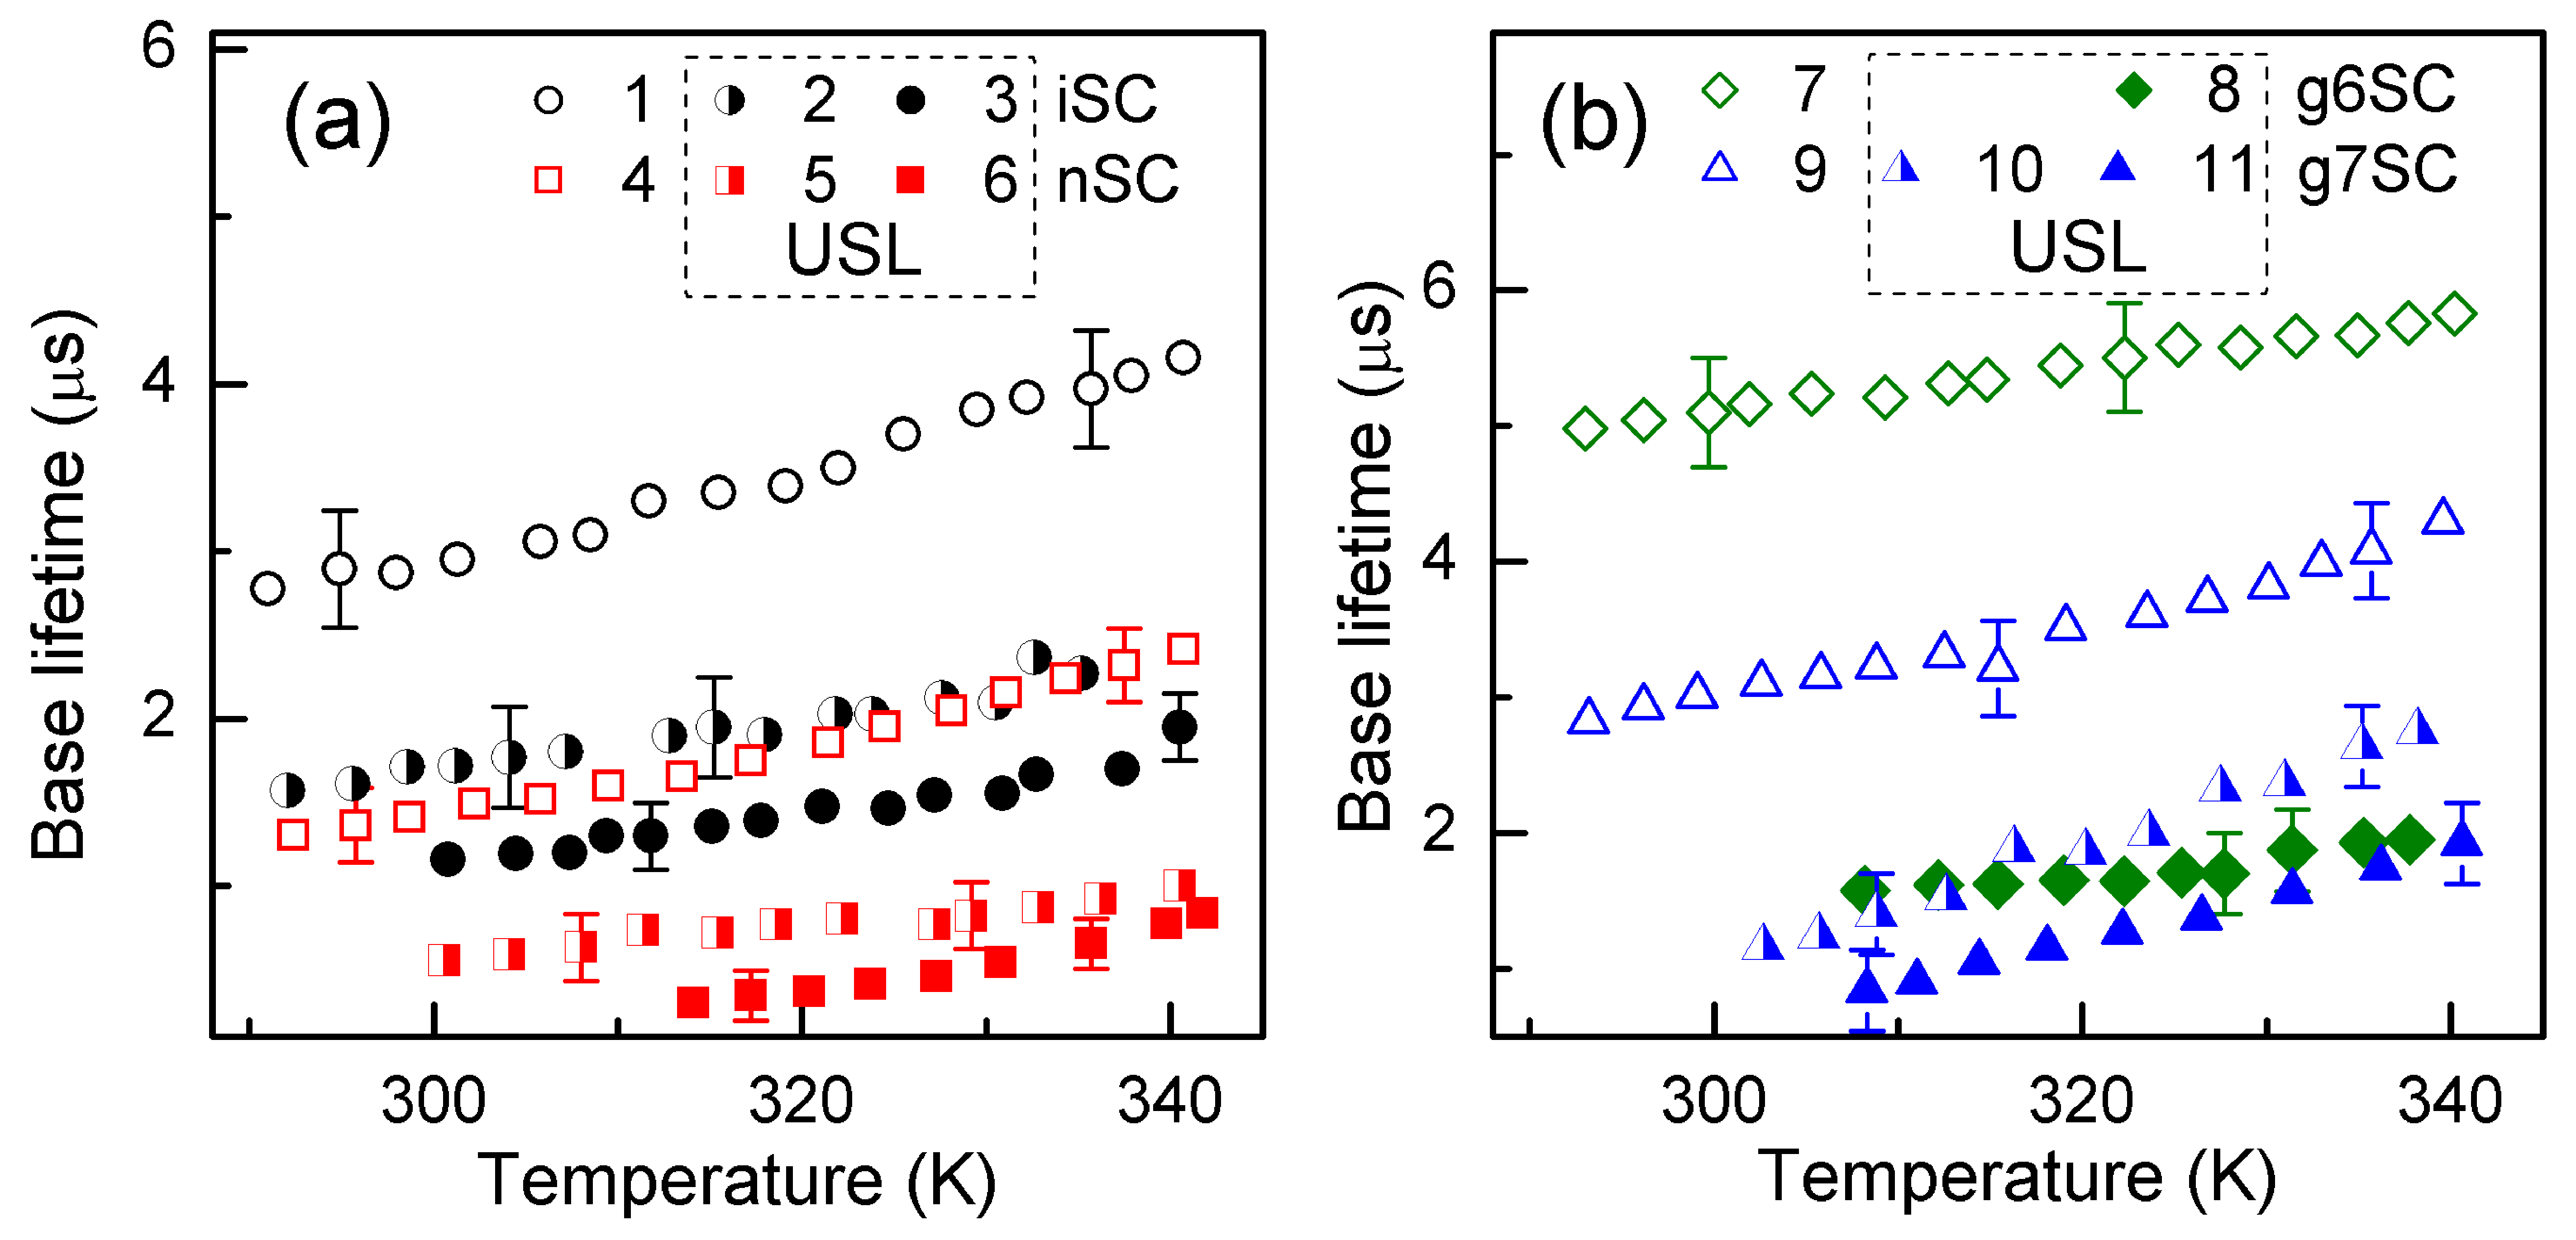
\includegraphics[width=0.7\textwidth]{fig_7ab}%
\caption{\label{fig_TAUr}
Temperature dependences of base lifetime for non--irradiated (curves 1--3, circles),
neutron--irradiated (4--6, squares) and $\gamma$--irradiated (7--11, diamonds and triangles) samples.
The curves 1, 4, 7 and 9 (open marks) are obtained without USL,
curves 2, 3, 5, 6, 8, 10, and 11 correspond to
Ui--1, Ui--2, Un--1, Un--2, Ug6--2, Ug7--1, and Ug7--2 respectively.
}%
\end{figure*}

Really, the irradiation induced lifetime reduction is described by the Messenger–-Spratt equation:\cite{Markvart}
\begin{equation}
\label{eqMS}
\tau_n^{-1}=\tau_{n0}^{-1}+K_\tau\Psi\,,
\end{equation}
where $\tau_{n0}$ is the minority carrier lifetime in the non--irradiated sample,
and $K_\tau$ is a lifetime damage--constants.
The known $K_\tau$ values and estimated changes of reciprocal base lifetime $K_\tau\Psi$ are shown in the Table~\ref{tabTAUn}.
It shows, that the estimated value of radiation--induced $\tau_n^{-1}$ change equals to ($8\div17$), 4, and 29~\% of
its measured value for samples nSC, g6SC, and g7SC respectively, and cannot explain dispersion observed experimentally.
Calculated lifetime changes $K_\tau\Psi$ are in quite good agreement with those, which are expected from RDs production --- see Section~\ref{DefectType}.

\begin{table}
\caption{\label{tabTAUn}Measured and estimated base lifetime parameters.
}
\begin{ruledtabular}
\begin{tabular}{ccccc}
\multirow{2}{*}{Sample} &$\tau_{n,in}^{-1}$ (320~K)&$K_\tau$&$K_\tau\times\Psi$ &$K_\mathtt{US}^\mathtt{eff}$ \\
&(10$^5$~s$^{-1}$)&(cm$^2/$s)& (10$^4$~s$^{-1}$)&(cm$^2/$W) \\
\hline
iSC&2.9&---&---&3.5\\
nSC&4.7&10$^{-7}$(Ref.~\onlinecite{NIEL:Jafari})&\multirow{2}{*}{4$\div$8}&7.1\\
&&2$\cdot$10$^{-7}$(Ref.~\onlinecite{n:Gaubas})&&\\
g6SC&1.8&5$\cdot$10$^{-12}$&0.8&6.0\\
g7SC&2.8&(Refs.~\onlinecite{NIEL:Jafari}, \onlinecite{gamma:Kolkov})&8&5.2\\
\end{tabular}
\end{ruledtabular}
\end{table}

Base lifetime can be expressed as following:\cite{MurphyJAP2011}
\begin{equation}
\label{eqTAUsum}
\tau_n^{-1}=\tau_\mathtt{bb}^{-1}+\tau_\mathtt{CE\,Auger}^{-1}+\tau_\mathtt{SRH}^{-1}\,,
\end{equation}
where
$\tau_\mathtt{bb}$, $\tau_\mathtt{CE\,Auger}$, $\tau_\mathtt{SRH}$ are the lifetimes of band--to--band, Coloumb--enhanced Auger, and
SRH recombination, respectively.
Calculation shows, that $\tau_\mathtt{bb}^{-1}=14$~s$^{-1}$, $\tau_\mathtt{CE\,Auger}^{-1}=6$~s$^{-1}$ and can be neglected.
In case of low injection level and single recombination centre, SRH lifetime is described by Eq.~(\ref{eqTAU}).
If there are  several centers of recombination the following equation should be applied
\begin{equation}
\label{eqTAUSHRsum}
\tau_n^{-1}=\sum_i^{M_d}\tau_{n,i}^{-1}=\sum_i^{M_d}N_{d,i},\sigma_{n,i}\,\upsilon_{\mathrm{th},n}\,,
\end{equation}
where
$M_d$ is the total number of centers,
$\tau_{n,i}$ characterizes lifetime due to recombination by $i$--th defect,
$N_{d,i}$ and $\sigma_{n,i}$ are the concentration and electron CCS of $i$--th defect, respectively.

Fig.~\ref{fig_TAUr} shows, that USL results in $\tau_n$ decrease.
Relative AI changes of reciprocal base lifetime $\varepsilon_{\tau n}=(\tau_{n,in}-\tau_{n,\mathtt{US}})/\tau_{n,\mathtt{US}}$
are listed in Table~\ref{tabAIchange}.
As AI changes is reversible, in our opinion, this effect deals with increase of $\sigma_n$ under US action.
Following the empirical relation  proposed by Ref.~\onlinecite{CDLR:R2}, we assume that Eq.~(\ref{eqSigma})
is correct for complex point defect too.
But in this case, $r$ is the distance, which separates components of complex.
According to the model suggested in Section~\ref{SCR}, USL leads to $r$ variation
and $\sigma_n$ change in line with Eq.~(\ref{eqEpsSig}).
In case of CDLR, AI change of donor (or/and acceptor) SSC is supplemental to variation of
both the coupling parameter and the couple distance.
But only change of SSC determines the AI variation of base lifetime.

On the other hand, not every defect effectively takes part in AID .
If  $M_d^\mathtt{AA}$ and $M_d^\mathtt{nonAA}$ are the total numbers of acoustically active (AA) and non--AA center,
Eq~(\ref{eqTAUSHRsum}) for $\tau_{n}^{-1}$ under USL and without it takes the following shape
\begin{eqnarray}
\tau_{n,in}^{-1}&=&\sum_j^{M_d^\mathtt{AA}}N_{d,j},\sigma_{n,j}^{in}\,\upsilon_{\mathrm{th},n}+
\sum_l^{M_d^\mathtt{nonAA}}N_{d,l},\sigma_{n,l}\,\upsilon_{\mathrm{th},n}\,,\nonumber\\
\tau_{n,\mathtt{US}}^{-1}&=&\sum_j^{M_d^\mathtt{AA}}N_{d,j},\sigma_{n,j}^\mathtt{US}\,\upsilon_{\mathrm{th},n}+
\sum_l^{M_d^\mathtt{nonAA}}N_{d,l},\sigma_{n,l}\,\upsilon_{\mathrm{th},n}\,.\nonumber
\end{eqnarray}
Using Eq~(\ref{eqEpsSig}), $\varepsilon_{\tau n}$  transforms as follows
\begin{equation}
\label{eqEpsTAU}
\varepsilon_{\tau n}=K_\mathtt{US}^\mathtt{eff}W_\mathtt{US}\,,
\end{equation}
where $K_\mathtt{US}^\mathtt{eff}$ characterizes ADI in the sample
and depends on concentration of both AA and non--AA centers
\begin{equation}
\label{eqKeff}
K_\mathtt{US}^\mathtt{eff}=\sum_j^{M_d^\mathtt{AA}}\frac{\tau_{n,in}}{\tau_{n,j,in}}K_\mathtt{US,j}\,,
\end{equation}
$K_\mathtt{US,j}$ deals with $j$--th defect--ultrasound interaction.

The obtained dependences $\varepsilon_{\tau n}$ vs $W_\mathtt{US}$ are shown in Fig.~\ref{fig_Kus}.
Linearity of these dependencies prove correctness of our assumptions.
The determined $K_\mathtt{US}^\mathtt{eff}$ values are listed in the Table~\ref{tabTAUn}.
The non--monotonic $K_\mathtt{US}^\mathtt{eff}$ alteration with $\gamma$ dose
is discussed in Section \ref{DefectType}.

\begin{figure}
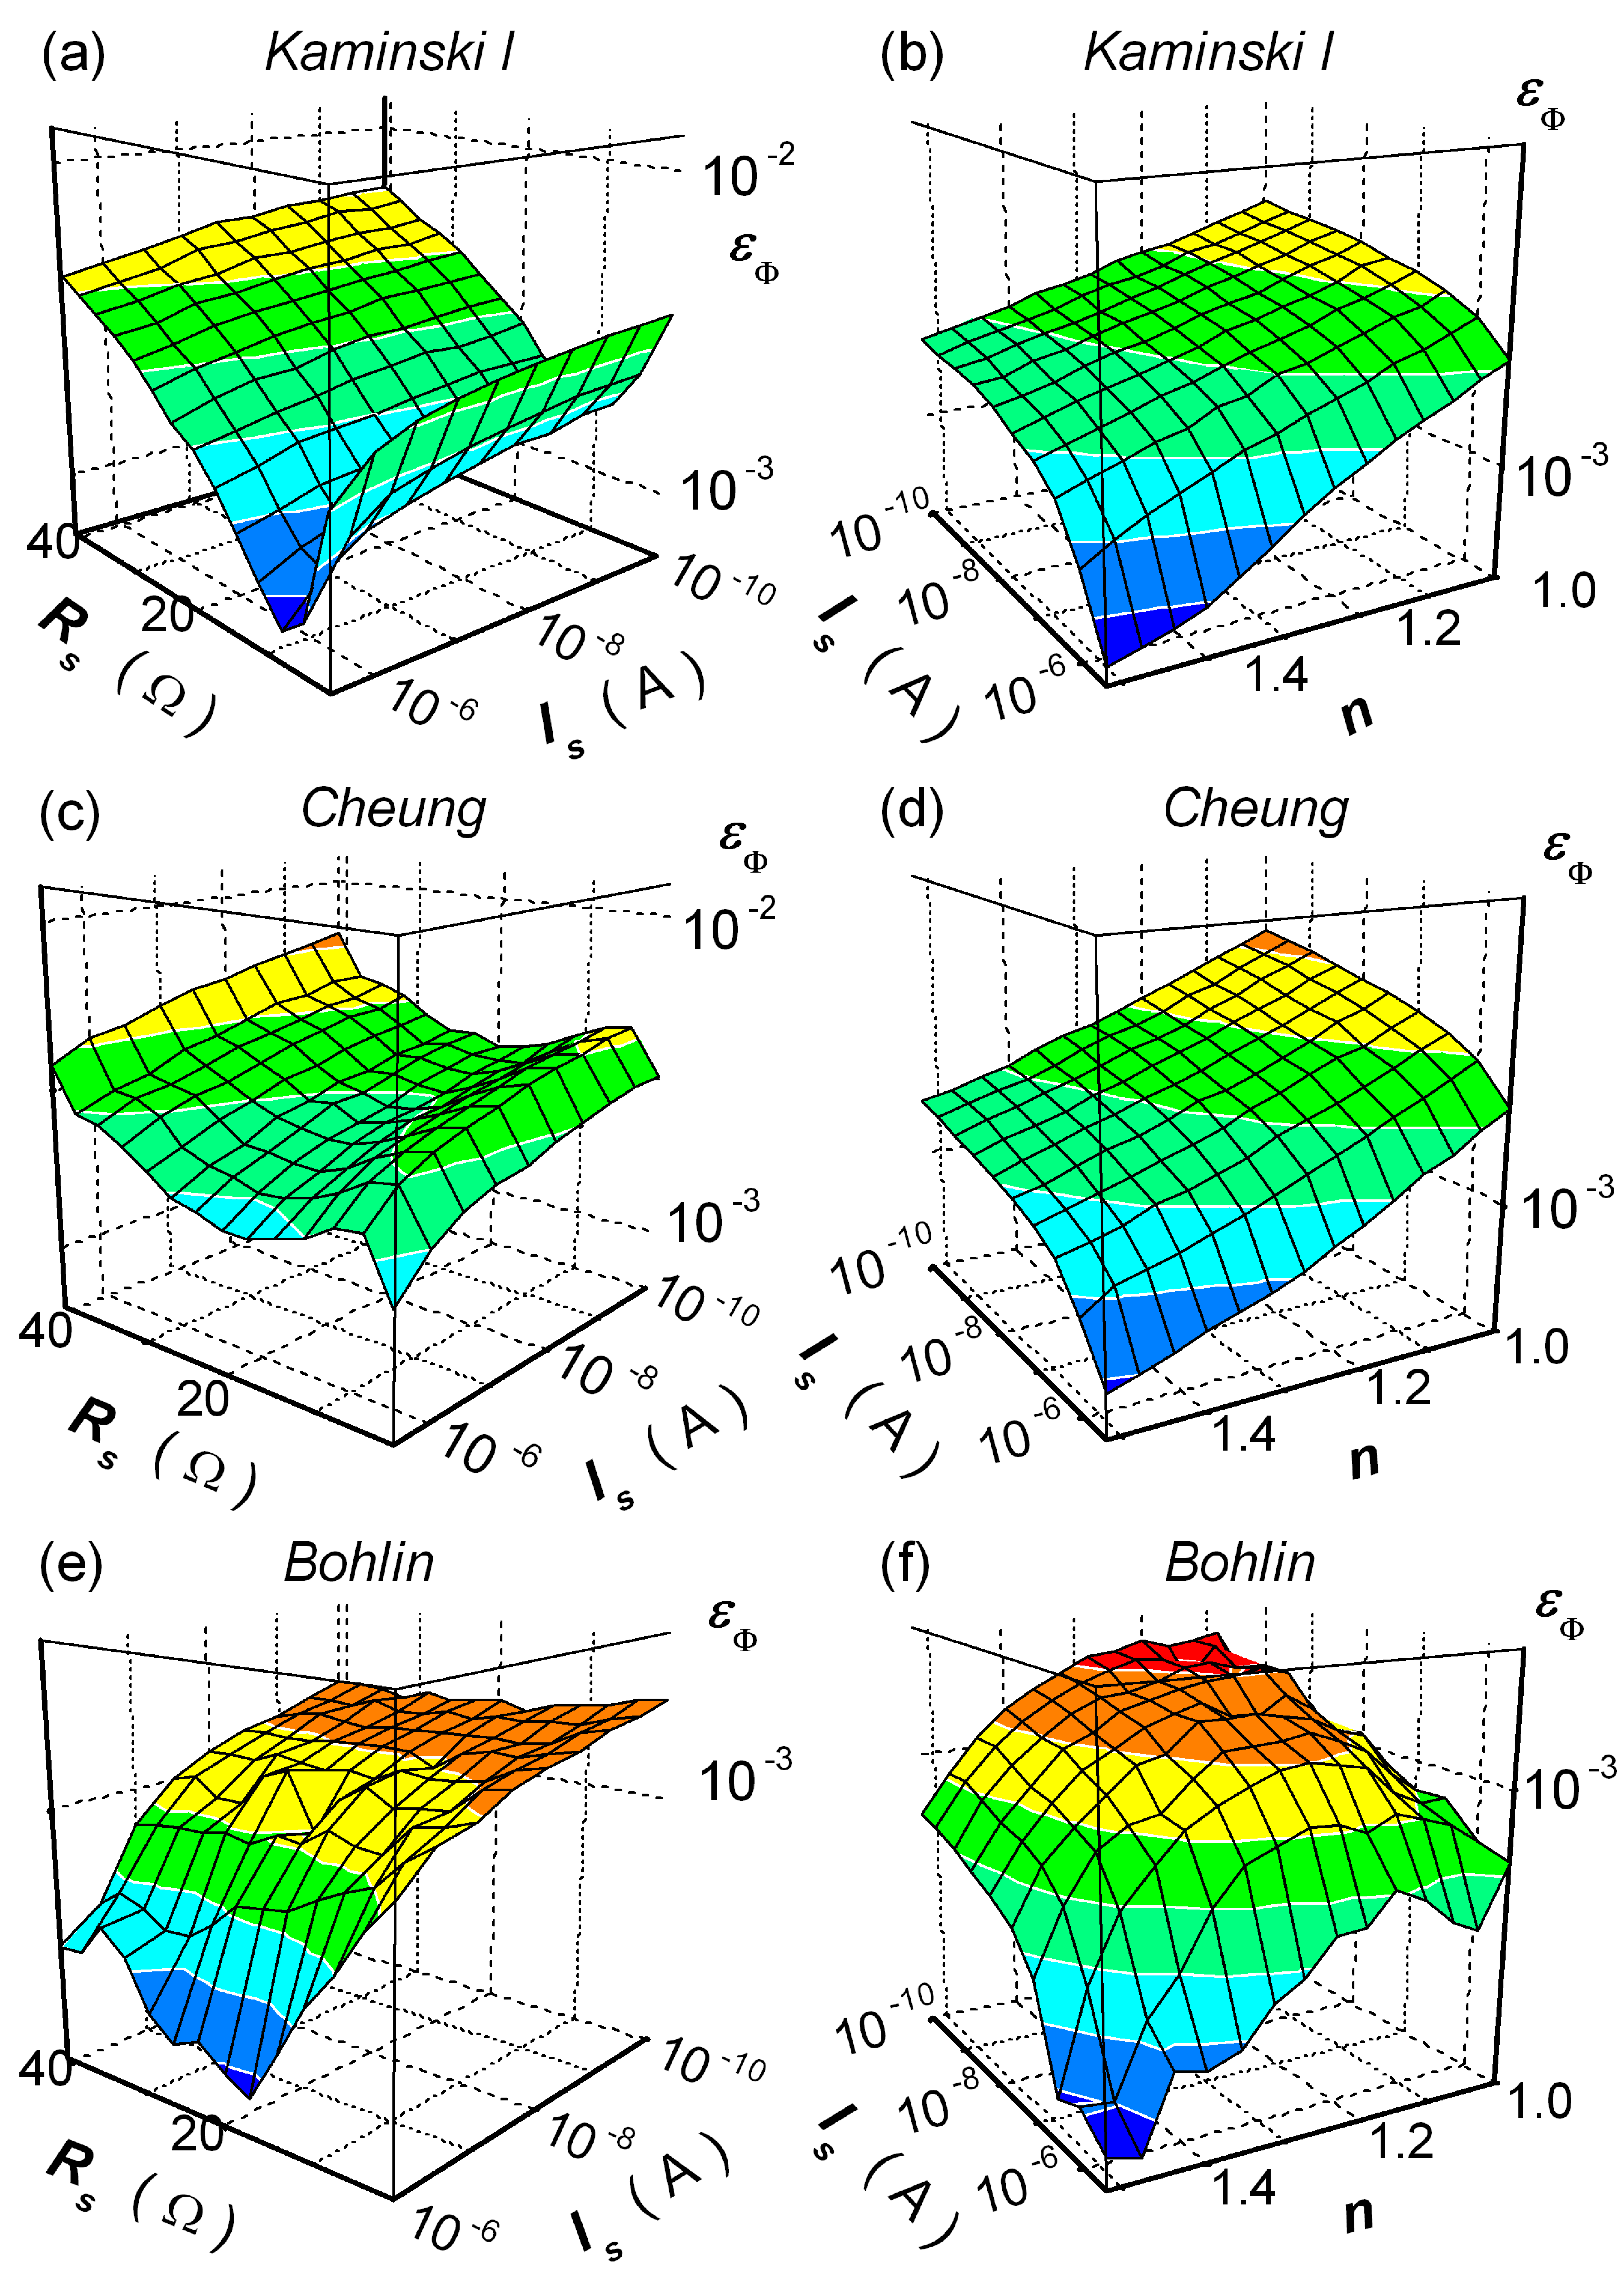
\includegraphics[width=0.45\textwidth]{fig_8}%
\caption{\label{fig_Kus}
Dependences of base lifetime relative change on US intensity for non--irradiated (circles), neutron--irradiated (squares), and $\gamma$--irradiated
(triangles and diamonds) samples.
Lines are the fitted curves using Eq.~(\ref{eqEpsTAU}).
}%
\end{figure}

\subsection{Shunt resistance\label{Rsh}}
Fig.~\ref{fig_Rsh} shows the  shunt resistance  over the explored temperature range.
One can see, that irradiation results in $R_{sh}$ decrease.
Besides the $R_{sh}$ temperature dependence behavior is changed in $\gamma$--exposed samples.
In particular  the shunt resistance decreases with the temperature growth in iSC and nSC,
whereas close to linear increase of $R_{sh}$ vs $T$  is observed in g6SC and g7SC at 293~K neighbourhood.
We want to notice that $R_{sh}$ axis is logarithmic in Fig.~\ref{fig_Rsh}(a) and linear in Fig.~\ref{fig_Rsh}(b).

\begin{figure*}
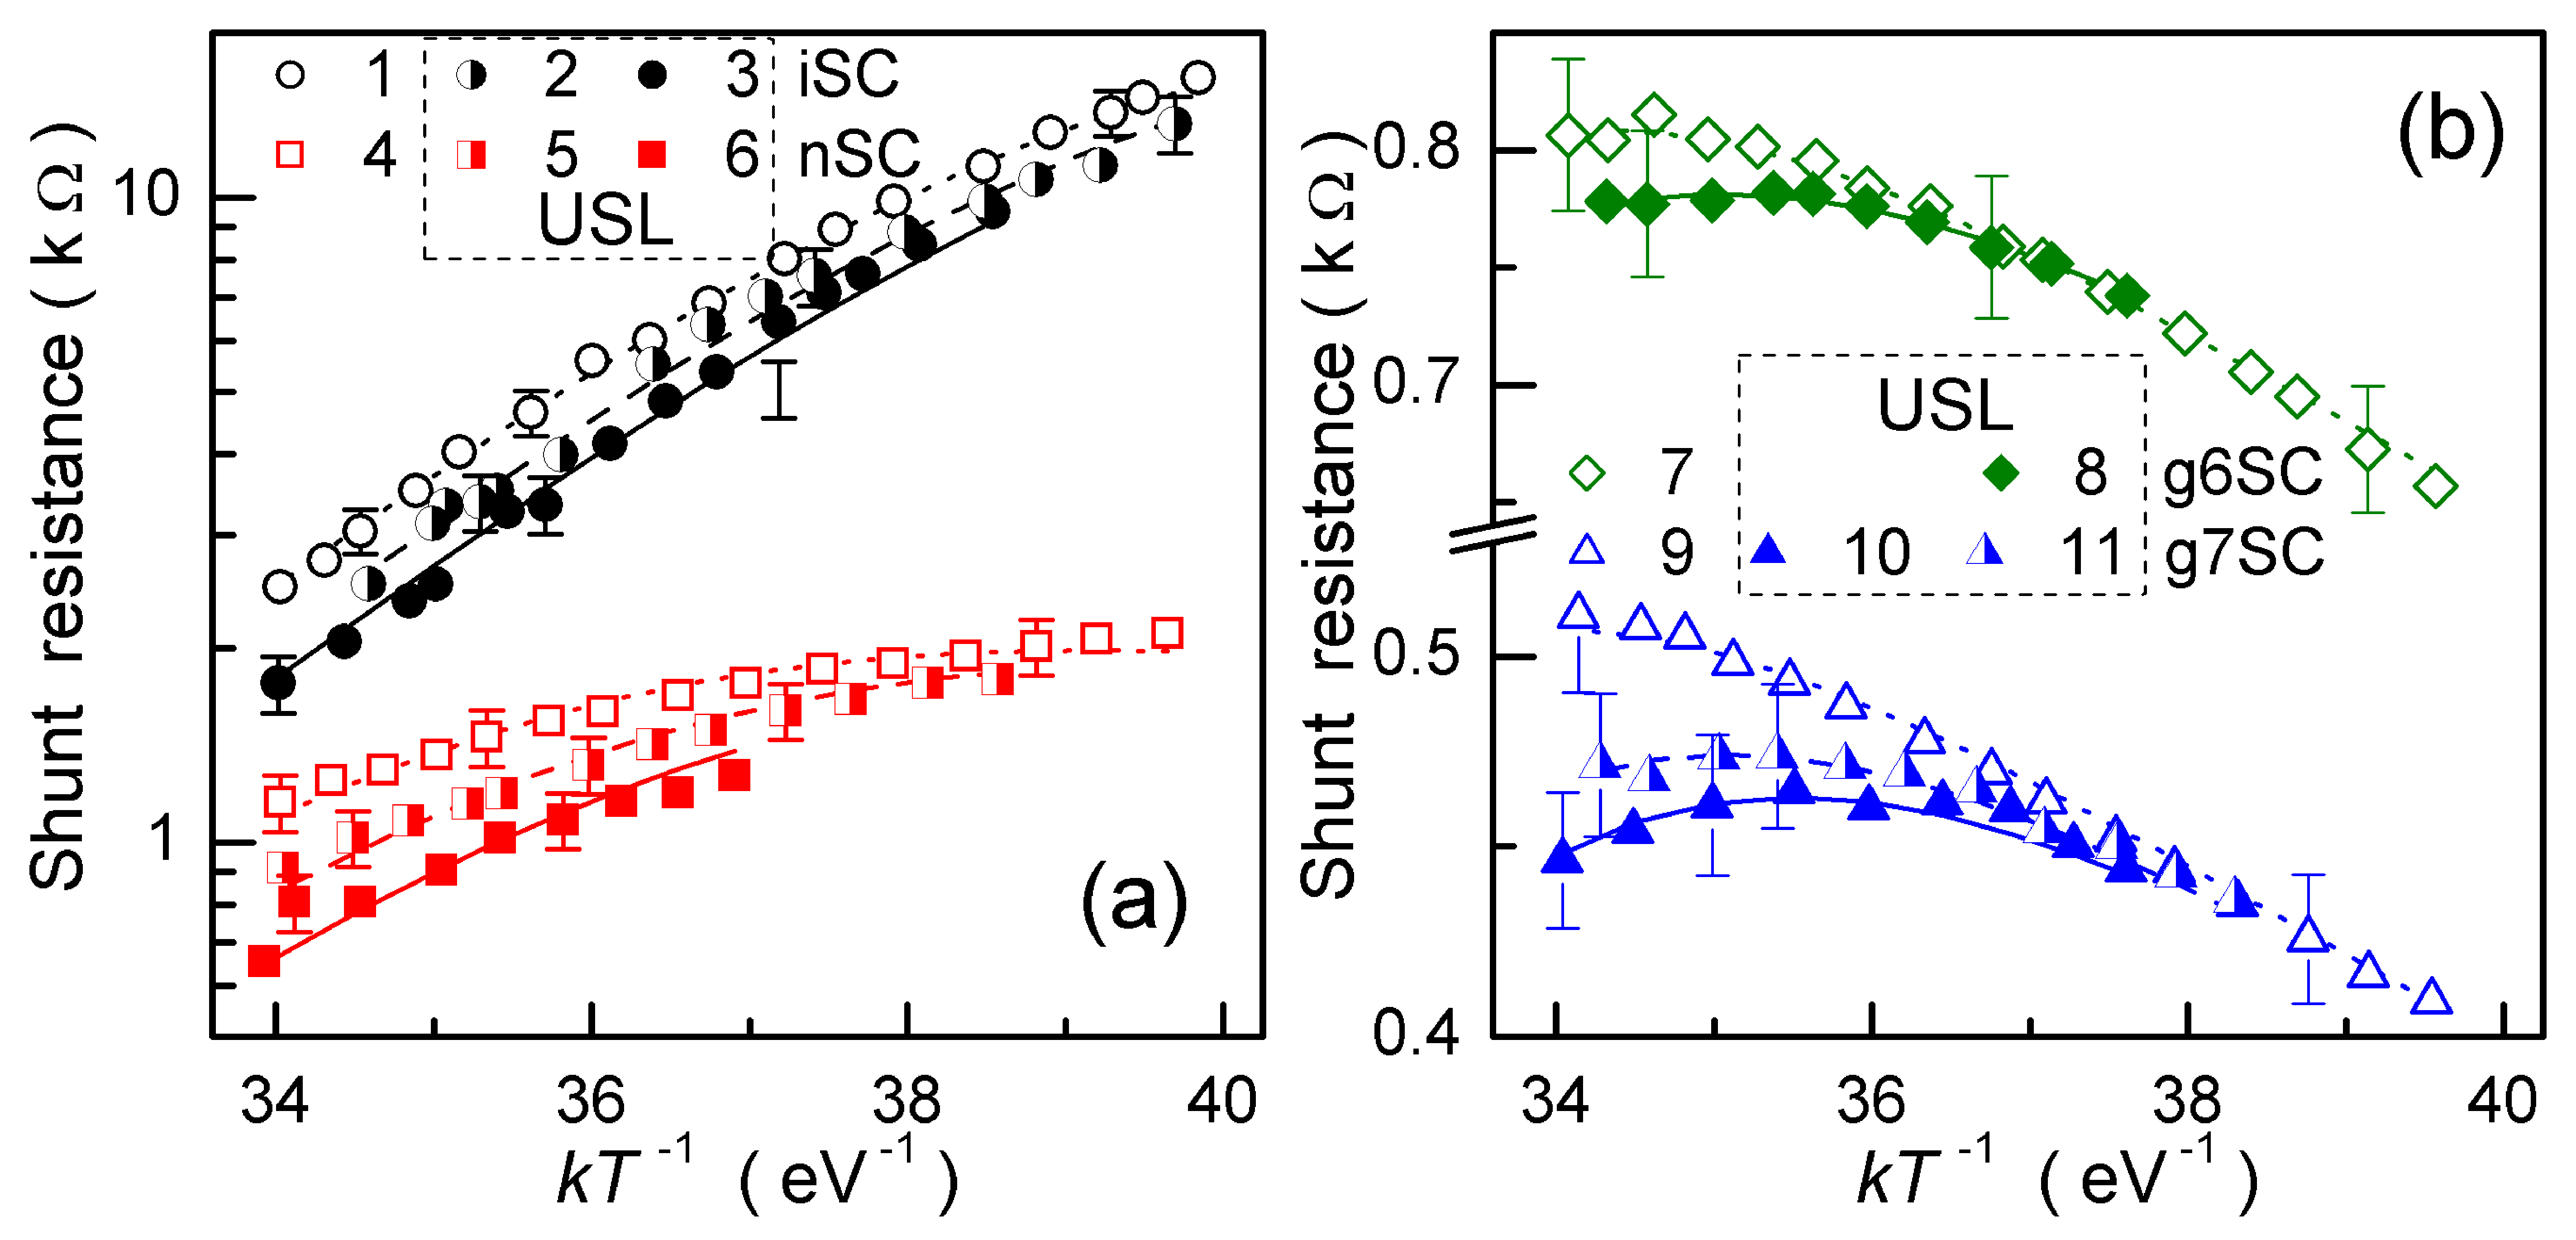
\includegraphics[width=0.7\textwidth]{fig_9ab}%
\caption{\label{fig_Rsh}
Temperature dependences of shunt resistance for non--irradiated (curves 1--3, circles),
neutron--irradiated (4--6, squares) and $\gamma$--irradiated (7--11, diamonds and triangles) samples.
The curves 1, 4, 7 and 9 (open marks) are obtained without USL,
curves 2, 3, 5, 6, 8, 10, and 11 correspond to
Ui--1, Ui--2, Un--1, Un--2, Ug6--2, Ug7--1, and Ug7--2 respectively.
The marks are the experimental results, the lines are the fitted curves using Eq.~(\ref{eqRshFull})-(\ref{eqRsh}).
}%
\end{figure*}

Several non-mechanical reasons of $p$--$n$ structure shunt resistance appearance are known.\cite{Rsh:Breitenstein}
They are aluminum particles, macroscopic Si$_3$N$_4$ inclusions, inversion layers at precipitates.
So in the course of firing Al particle may penetrate into the sample creating $p^+$--doped region around it, which compensates the emitter and stay in ohmic contact with the
base.
Inversion layers and Si$_3$N$_4$ inclusions occur in multicrystalline silicon cells mainly \cite{Rsh:Breitenstein} and cannot cause a shunt resistance of investigated samples.
In addition, dislocations, which intersect the junction, are generally held responsible as a possible source of ohmic current.\cite{Rsh:Breitenstein,TAT:Gopal,Rsh:Baker}
In our opinion, both aluminum particles and dislocations are present in the investigated structure.
The overall shunt resistance can be expressed as
\begin{equation}
\label{eqRshFull}
R_{sh}^{-1}=R_{sh,\mathtt{Al}}^{-1}+R_{sh,\mathtt{dis}}^{-1}\,,
\end{equation}
where
$R_{sh,\mathtt{Al}}$ and $R_{sh,\mathtt{dis}}$ deal with aluminum particles and dislocations, respectively.
The linear temperature dependence of metal particles $R_{sh,\mathtt{Al}}$ is suggested:
\begin{equation}
\label{eqRshAl}
R_{sh,\mathtt{Al}}=R_{293,\mathtt{Al}}[1+\alpha(T-293)]\,,
\end{equation}
where
$R_{293,\mathtt{Al}}$ is the shunt resistance at 293~K and
$\alpha$ is the resistance temperature coefficient.

Gopal and Gupta \cite{Rsh:Gopal2003,Rsh:Gopal2004} introduced the model of dislocation--induced impedance of photovoltaic detector.
According to this model, the $R_{sh,\mathtt{dis}}$ can be given by
\begin{equation}
\label{eqRsh}
R_{sh,\mathtt{dis}}=\frac{T}{\sigma_{\mathtt{dis}}}\left[\cosh\left(\frac{E_\mathtt{dis}-E_i}{kT}\right)+\cosh\left(\frac{U_s}{kT}\right)\right]\,,
\end{equation}
with
\begin{equation}
\label{eqRdis}
%\sigma_{\mathtt{dis}}=\rho_{\mathtt{dis}}Aq^2A_{\mathtt{dis}}\sqrt{K_nK_p}\,N_{\mathtt{dis}}(n_p+p_p)k^{-1}\,,
\sigma_{\mathtt{dis}}=\rho_{\mathtt{dis}}Aq^2A_{\mathtt{dis}}\sqrt{K_nK_p}\,N_{\mathtt{dis}}(n_p+p_p)/k\,,
\end{equation}
where
$E_{\mathtt{dis}}$ is the energy level which significantly contributes to the dislocation recombination current,
$U_s$ is the potential at the surface of the dislocation core,
$\rho_{\mathtt{dis}}$ and $A_{\mathtt{dis}}$ are the dislocation density and surface area, respectively,
$K_n$ and $K_p$ are the capture probabilities for electrons and holes by the dislocation states,
$N_{\mathtt{dis}}$ is the density of surface states at each dislocation.
Eq.~(\ref{eqRsh}) is correct in simplified case of $K_p=K_n$.

$\alpha$ was determined from g7SC data.
Obtained value $8.3\cdot10^{-3}$~K$^{-1}$ is not far from resistance temperature coefficient of bulk Al ($4.3\cdot10^{-3}$~K$^{-1}$).
Then we used Eqs.~(\ref{eqRshFull})--(\ref{eqRsh}) to fit the experimental $R_{sh}$ data.
$R_{293,\mathtt{Al}}$, $(E_{\mathtt{dis}}-E_i)$, $U_s$, and $\sigma_{\mathtt{dis}}$ were taken as the fitting parameters.
It was established that the experimental data are in good agreement with the fitting curves (see Fig.~\ref{fig_Rsh}) for values $(E_{\mathtt{dis}}-E_i)=(0.46\pm0.02)$~eV and $U_s=(5\pm4)\times10^{-8}$~eV, which were independent of irradiation and USL.
The obtained value of $(E_{\mathtt{dis}}-E_i)$ corresponds to the carrier activation energy $0.10\pm0.02$~eV.
This value is comparable to the
activation energy of dislocation levels $0.08$~eV,
which was early reported\cite{disl10:Castaldini,disl10:Isakova,disl10:Yu,disl10:Kveder,disl10:Trushin}
in Cz--Si:B too.\cite{disl10:Castaldini,disl10:Isakova,disl10:Yu}



Obtained values of $R_{293,\mathtt{Al}}$ and $\sigma_{\mathtt{dis}}$ are listed in the Table~\ref{tabTpar}.
$R_{293,\mathtt{Al}}$ does not depend on USL and increases with irradiation level.
In our opinion, $R_{sh,\mathtt{dis}}$ is less than $R_{sh,\mathtt{Al}}$ in iSC.
Irradiation leads to vacancy production and Al diffusion out of electrodes.
As a result, the quantity of Al particles rises, $R_{sh,\mathtt{Al}}$ decreases and becomes the key factor of overall shunt resistance value.
The Al diffusion is more effective in $\gamma$--exposed samples due to more uniform distribution of irradiation--induced single vacancies.

Dispersions of $\sigma_{\mathtt{dis}}$ and $\tau_n$ correlate on samples set.
Hence it deals with wafer inhomogeneity too.
USL leads to $\sigma_{\mathtt{dis}}$ increase, relative AI changes
$\varepsilon_{\sigma\mathtt{dis}}=(\sigma_{\mathtt{dis,US}}-\sigma_{\mathtt{dis},in})/\sigma_{\mathtt{dis},in}$
are shown in the Table~\ref{tabAIchange}.
In our opinion this is caused by an $A_\mathtt{dis}$ augmentation.
Namely, the dislocation core atom displacement  is  normal to the  current direction.
As the result, carriers are captured by dislocation levels from enlarged volume.
Therefore the effective surface area increases and L$R_{sh,\mathtt{dis}}$ decreases under US action.


\subsection{Defect type speculation\label{DefectType}}

Lifetime killers  in boron--doped Czochralski--grown Si are the  boron--oxygen related (BO) defects,\cite{LIDRev,LIDRev2}
iron--boron pairs \cite{MurphyJAP2011,FeB:Vahanissi,FeB:Schmidt} (or another Fe--related trap in the $n^+p$--junctions \cite{TeimurazPSS,TeimurazJAP}),
and oxide precipitates.\cite{MurphySC2014,Oxide_Schon,MurphyJAP2011,MurphyJAP2012,Oxide:Chen,Oxide:Porrini}
The first two defects are sensitive to intensive illumination at room temperature.
To determine the major recombination center of investigated samples the following experimental procedure has been used.
The non-irradiated sample was light soaked under halogen lamp (2 Suns) illumination at approximately 305~K.
The illumination varied from 1~h to 8~h.
After illumination sample is stored in the dark at room temperature.
To determine the kinetics of parameters the $I$--$V$ characteristics have been measured with interval 10--15~min at room temperature over a period 5~h after illumination stopping.
To determine the permanent light--induced change the $I$--$V$ characteristics have been measured in 48~h after illumination.
After accumulated time under illumination had run up to 15~h the iSC was annealed at 200~$^\circ$C for $10$~min in the dark and measurements were made at room temperature.
After that, the illumination and measurements were repeated.


\begin{figure}
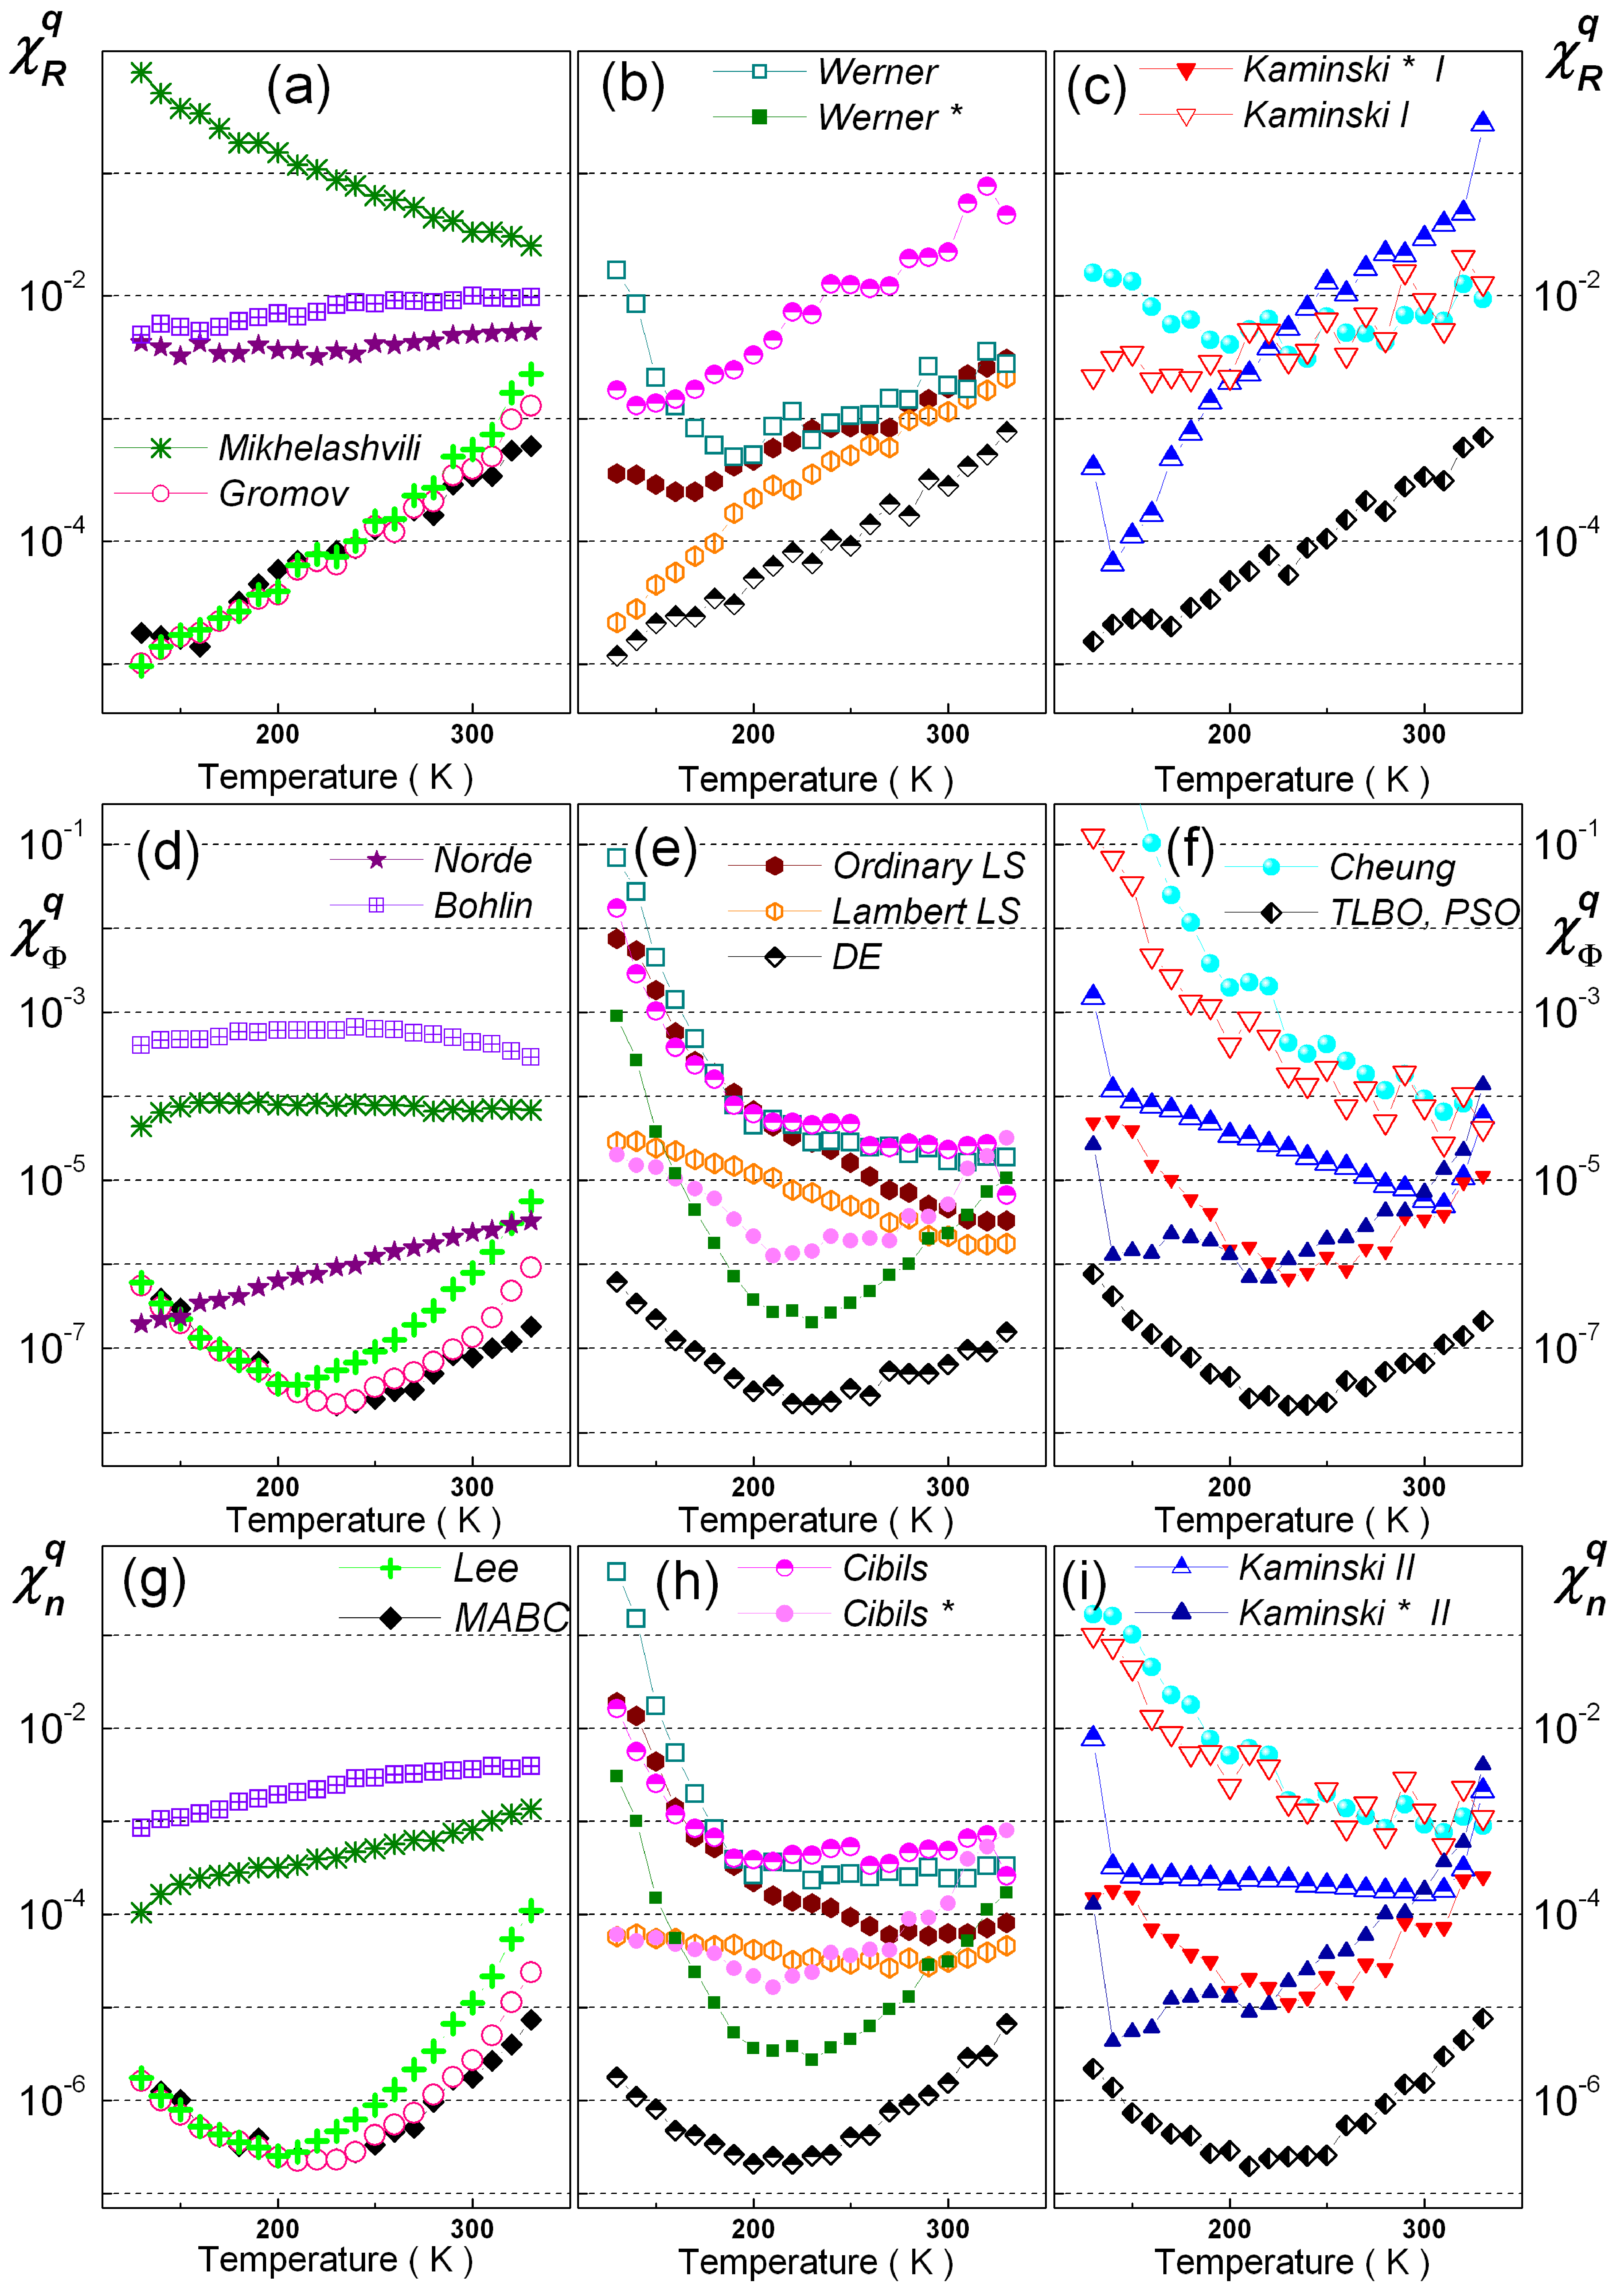
\includegraphics[width=0.46\textwidth]{fig_10}%
\caption{\label{fig_Illum}
Permanent changes of SCR lifetime (a, squares), ideality factor (b, circles), base lifetime (c, triangles), and shunt resistance (d, asterisks) versus accumulated illumination time.
Sample iSC, $T=295$~K.
Filled, semi--filled and open marks correspond to sample before annealing, after first $10$~min 200~$^\circ$C annealing, and after second $10$~min 200~$^\circ$C annealing, respectively.
}%
\end{figure}

Intensive light is known\cite{LIDRev,LIDRev2} to lead to permanent transformation of BO defects and considerable decrease of minority--carrier lifetime (down to 10~\% of initial value at long term illumination).
Annealing at 200~$^\circ$C for $10$~min in the dark results in both BO defects state recovery and readiness of light--induced degradation.
Fig.~\ref{fig_Illum} show changes of structure parameters in comparison with those before illumination.
One can see that illumination did not result in considerable permanent change of either of the $\tau_g$, $\tau_n$, $n_{\mathrm{id}}$ before as well as after annealing.
Therefore BO influence on recombination can be neglected  in both the SCR and the base.

On the other hand, the vast majority of impurity iron exists in iron--boron pairs.
Fe$_i$B$_s$ can be readily dissociated under intense illumination to release interstitial iron.
This gives a lifetime change.
In dark Fe$_i$B$_s$ repairing takes place and Fe$_i$ concentration decreases according to \cite{MurphyJAP2011,Wijaranakula}
\begin{equation}
\label{eqFeB}
N_{Fe}(t)=(N_{Fe,\,0}-N_{Fe,\,eq})\exp\left[-\frac{t}{\tau_{\mathtt{rep}}}\right]+N_{Fe,\,eq}\,,
\end{equation}
where
$N_{Fe,\,0}$ and $N_{Fe,\,eq}$ are the concentration after illumination immediately and equilibrium
concentration which remains a long time after dissociation respectively,
and the characteristic time of repairing $\tau_{\mathtt{rep}}$ depends on doping level
\begin{equation}
\label{eqTrep}
\tau_{\mathtt{rep}}=770\cdot p_p^{\,-2/3}\exp\left(\frac{E_{\mathtt{D,\,Fe}}}{kT}\right)\,,
\end{equation}
$E_{\mathtt{D,\,Fe}}=0.68$~eV is the activation energy of Fe$_i$ diffusion.

\begin{figure}
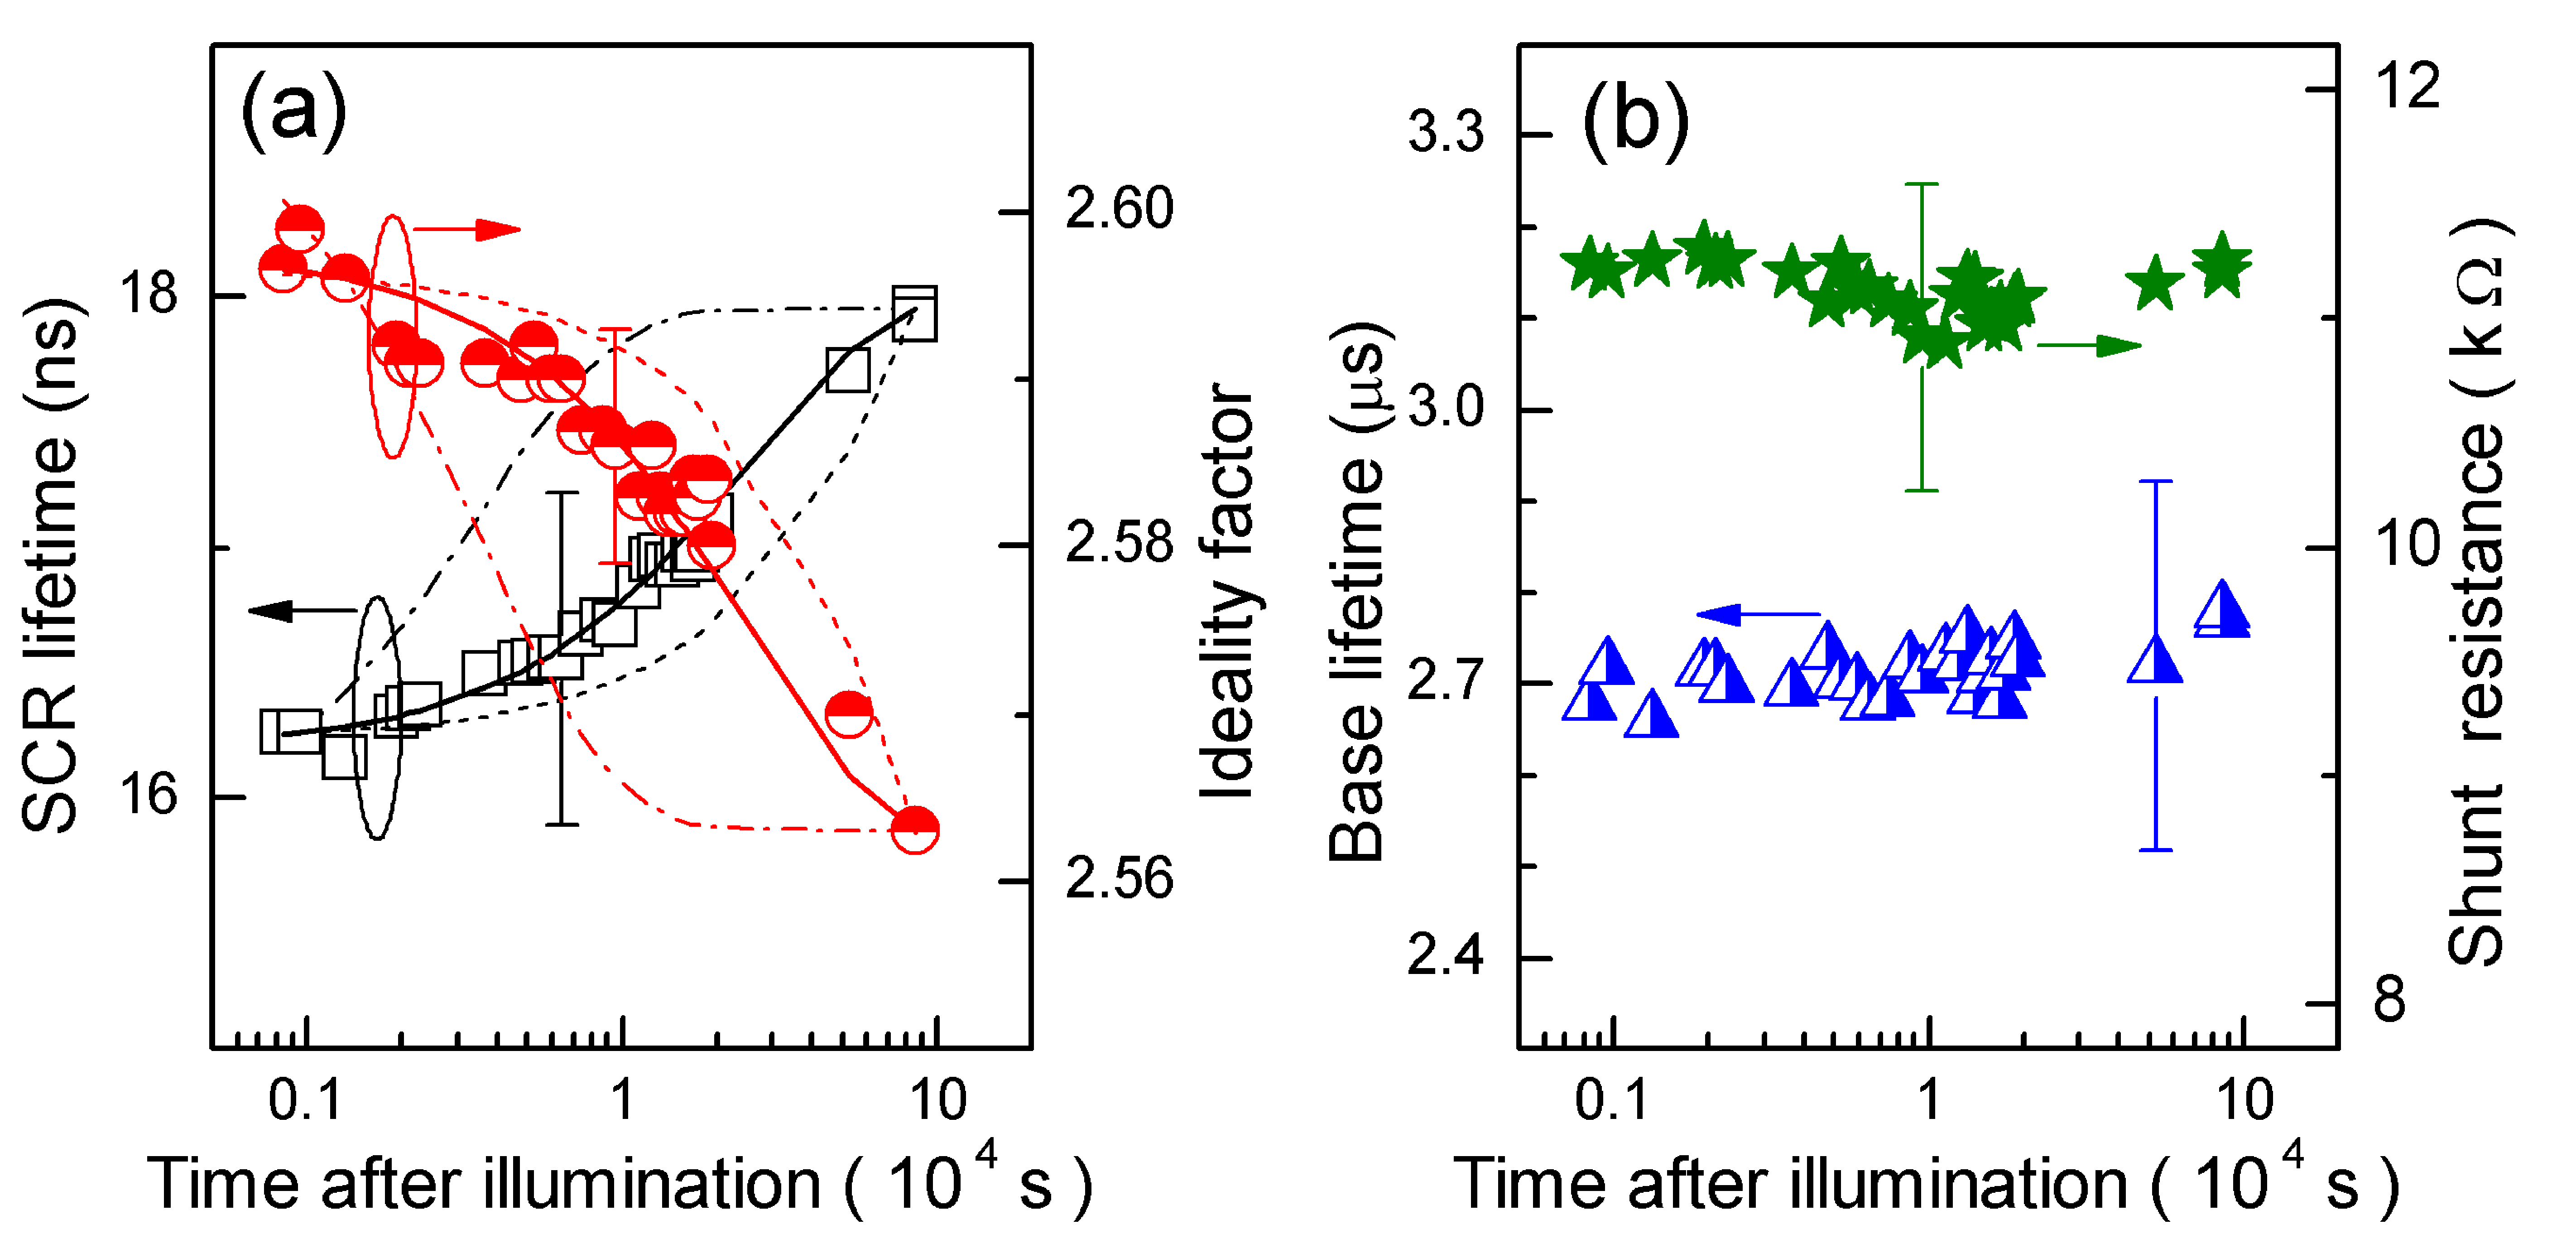
\includegraphics[width=0.47\textwidth]{fig_11ab}%
\caption{\label{fig_Time}
SCR lifetime (a, squares, left axis), ideality factor (a, circles, right axis), base  lifetime (b, triangles, left axis), and shunt resistance (b, asterisks, right axis) as a function of time since illumination stoping.
Sample iSC, $T=295$~K.
Lines are calculated by using Eqs.(\ref{eqFeB})--(\ref{eqTrep}) and $E_{\mathtt{D,Fe}}=0.63$~eV (dash--dotted lines), 0.68~eV (solid lines), and 0.73~eV (dashed lines).
}%
\end{figure}

$n_{\mathrm{id}}$ increase (about 0.03) and $\tau_g$ decrease (about 10~\%) immediately after illumination were observed --- see Fig.~\ref{fig_Time}(a).
These changes vanished gradually.
We supposed that the $\tau_g$ and $n_{\mathrm{id}}$ evolutions could be described by expressions, which like to Eq.~(\ref{eqFeB}).
Then Eq.~(\ref{eqTrep}) was used to calculate characteristic time and fitting lines were plotted on Fig.~\ref{fig_Time}(a).
The fittings with $E_{\mathtt{D,Fe}}=0.68$~eV are in good agreement with experimental data.
Hence iron--boron pairs take part in SCR recombination.
On the other hand, electron and hole CCS of Fe$_i$ are 1.7 and 0.04 times \cite{MurphyJAP2011} as much as those of Fe$_i$B$_s$.
A small (about 10~\%) $\tau_g$ alteration, which is caused by light, is evidence of supporting role of iron--boron pair in SCR recombination.
Furthermore, since $\tau_n$ does not depend on illumination (see Fig.~\ref{fig_Time}(b)), then Fe$_i$B$_s$ does not influence on base lifetime.

As a result, oxide precipitates are number one in SCR and base recombination.
According to Murphy \emph{et al}.\cite{MurphySC2014,MurphyJAP2012},
at least two independent oxide precipitate related defects exist.
These defects have $\sigma_n/\sigma_p=157$ and $\sigma_p/\sigma_n=1200$ respectively.\cite{MurphyJAP2012}
So, they are suitable for CDLR.
On the basis of mentioned above, we conclude that the defect, responsible for AI phenomena in nSC, is oxide precipitate mainly.

It is worth keeping doping level, oxygen concentration and irradiation dose in mind when RD type is foreseen.
In our case (Czochralski, oxygen--rich, $\sim7\cdot10^{17}$~cm$^{-3}$, $p$--Si with boron concentration $\sim10^{15}$~cm$^{-3}$ and low dose)
it is expected, that C$_i$O$_i$, vacancy clusters V$_n$ (divacancy V$_2$, trivacancy V$_3$, ...) and VO$_i$
are produced mainly by neutron irradiation \cite{n:long,n:gamma,Moll:PhD}
and C$_i$O$_i$ and  VO$_i$ by $\gamma$--rays.\cite{gamma:Stahl,Moll:PhD,gamma:Kolk,A:Caracas}
The RD concentration $N_{t,\mathtt{RD}}$ is proportionate to dose,
the known introduction rate for neutron $\eta_n$ and gamma $\eta_\gamma$ irradiation in Cz--Si are shown in the Table~\ref{tabDefect}.
The expected values of $N_{t,\mathtt{RD}}$ for investigated samples are listed in the Table~\ref{tabDefect} too.


\begin{table*}
\caption{\label{tabDefect}Cited and calculated defect parameters.
}
\begin{ruledtabular}
\begin{tabular}{cccccccccc}
Defect&$\sigma_n$&$\eta_n$ (cm$^{-1}$)&$\eta_\gamma$&\multicolumn{3}{c}{$N_{t,\mathtt{RD}}$(10$^{11}$~cm$^{-3}$)}&\multicolumn{3}{c}{$\tau_{n,\mathtt{RD}}^{-1}$ (10$^4$~s$^{-1}$)}\\
&(10$^{-15}$~cm$^2$)&Ref.~\onlinecite{Moll:PhD}&&nSC&g6SC&g7SC&nSC&g6SC&g7SC\\
\hline
C$_i$O$_i$&0.7 (Ref.~\onlinecite{gamma:Stahl})&1.38&6$\cdot$10$^5$~rad$^{-1}$cm$^{-3}$ (Ref.~\onlinecite{gamma:Stahl})&5.5&6&60&$0.8\div1$&$0.9\div1.1$&$9\div11$\\
&0.9 (Ref.~\onlinecite{gamma:Kolk})&&4$\cdot$10$^{-4}$~cm$^{-1}$ (Ref.~\onlinecite{gamma:Kolk})&&&&&&\\
V$_2$&3 (Ref.~\onlinecite{gamma:Stahl})&1.21&3$\cdot$10$^4$~rad$^{-1}$cm$^{-3}$ (Ref.~\onlinecite{gamma:Stahl})&4.8&0.3&3&$2.2\div3.3$&$0.1\div0.2$&$1\div2$\\
&2 (Ref.~\onlinecite{A:Brothe})&&&&&&&&\\
V$_3$&2.4 (Ref.~\onlinecite{V3:Markevich})&0.37&---&1.5&---&---&0.7&---&---\\
VO$_i$&2.4 (Ref.~\onlinecite{A:Caracas})&0.52&7$\cdot$10$^5$~rad$^{-1}$cm$^{-3}$ (Ref.~\onlinecite{gamma:Stahl})&2&$6\div7$&$60\div70$&&&\\
&4 (Ref.~\onlinecite{A:Bleicher})&&4$\cdot$10$^{-4}$~cm$^{-1}$ (Ref.~\onlinecite{gamma:Kolk})&&&&&&
\end{tabular}
\end{ruledtabular}
\end{table*}


Another defects, which can be created by irradiation in silicon, are I$_p$--center, bistable donor (BD), B$_i$O$_i$ and C$_i$C$_s$.
But I$_p$--center and BD are characterized by small introduction rate.
For example, expected\cite{n:gamma,BD:Fret} concentration of BD is only $(1\div2)\cdot10^{10}$~cm$^{-3}$ in nSC and g7SC.
The lack of B$_i$O$_i$ in investigated samples deals with low boron concentration \cite{SiIntDef}.
Lastly,  C$_i$C$_s$ creation is suppressed in oxygen--rich crystal.\cite{gamma:Kolk,gamma:Stahl,n:long}
Besides C$_i$C$_s$ is not recombination active center.\cite{CiCs:Song}

The influence of RD on base lifetime could be estimated by Eq.~(\ref{eqTAUSHRsum}) taking into account the fact, that
VO$_i$ is not active recombination center in $p$--Si.\cite{gamma:Kolkov,IrrCzpSi:Benton,IrrCzpSi:Coffa,IrrCzpSi:Ganagona,IrrCzpSi:Vines}
Estimated $\tau_{n,\mathtt{RD}}$ for C$_i$O$_i$, V$_2$, and  V$_3$ are shown in Table~\ref{tabDefect}.
It shows that  $\tau_n$ is effected mainly by C$_i$O$_i$ and vacancy clusters in $\gamma$-- and neutron--irradiated samples, respectively.
It should be noted, that nSC, g6SC, g7SC sums of $\tau_{n,\mathtt{RD}}$ are in quite good agreement with $(K_\tau\cdot\Psi)$ values.

Lets consider $K_\mathtt{US}^\mathtt{eff}$ assuming that
$M_d^\mathtt{AA}=1$, $M_d^\mathtt{nonAA}=1$ in non--irradiated sample and
US interaction with C$_i$O$_i$ and V$_n$ is described by $K_\mathtt{US}^\mathtt{CO}$ and $K_\mathtt{US}^\mathtt{V}$, respectively.
Then Eq.~(\ref{eqKeff}) gives the following expression for $K_\mathtt{US}^\mathtt{eff}$
in nSC and irradiated samples:
\begin{eqnarray}
K_\mathtt{US}^\mathtt{eff}&=&K_\mathtt{US}^\mathtt{AA}\,\tau_{n,in}/\tau_{n,in}^\mathtt{AA}\,,\nonumber\\
K_\mathtt{US}^\mathtt{eff}&=&K_\mathtt{US}^\mathtt{AA}\tau_{n,in}/\tau_{n,in}^\mathtt{AA}+
                           K_\mathtt{US}^\mathtt{CO}\tau_{n,in}/\tau_{n,\mathtt{RD}}^\mathtt{CO}+
                           K_\mathtt{US}^\mathtt{V}\tau_{n,in}/\tau_{n,\mathtt{RD}}^\mathtt{V} \,.\nonumber
\end{eqnarray}
$\tau_{n,in}^\mathtt{AA}$ is the base lifetime of the sample, where non-radiative AA defect with $K_\mathtt{US}^\mathtt{AA}$ is present only.


Two extreme cases are opportune for analysis.
In the first one, non--AA defects are distributed uniformly across the wafer and
AA defects define a distinction of
$(\tau_{n,in}^{-1}-K_\tau\cdot\Psi)$ values in different samples.
In the second one, a non--AA defect distribution is not uniform,
whereas $\tau_{n,in}^\mathtt{AA}$ is identical for iSC, nSC, g6SC, and g7SC.
However, in the first case (as well as in case of $M_d^\mathtt{nonAA}=0$),
experimental $K_\mathtt{US}^\mathtt{eff}$ values lead to unreal (negative) values of $K_\mathtt{US,j}$.
In the second case, Eq.~(\ref{eqKeff}) and the data from the Tables~\ref{tabTAUn} and \ref{tabDefect}, give the following array equations:
\begin{eqnarray}
\mbox{iSC}:\,\,3.5&=&K_\mathtt{US}^\mathtt{AA}\cdot(\tau_{n,in}^\mathtt{AA})^{-1}\,/2.9\,,\nonumber\\
\mbox{nSC}:\,\,7.1&=&K_\mathtt{US}^\mathtt{AA}\cdot(\tau_{n,in}^\mathtt{AA})^{-1}\,/4.7+0.09\,K_\mathtt{US}^\mathtt{V}+0.02\,K_\mathtt{US}^\mathtt{CO}\,,\nonumber\\
\mbox{g6SC}:\,\,6.0&=&K_\mathtt{US}^\mathtt{AA}\cdot(\tau_{n,in}^\mathtt{AA})^{-1}\,/1.8+0.01\,K_\mathtt{US}^\mathtt{V}+0.05\,K_\mathtt{US}^\mathtt{CO}\,,\nonumber\\
\mbox{g7SC}:\,\,5.2&=&K_\mathtt{US}^\mathtt{AA}\cdot(\tau_{n,in}^\mathtt{AA})^{-1}\,/2.8+0.05\,K_\mathtt{US}^\mathtt{V}+0.35\,K_\mathtt{US}^\mathtt{CO}\,,\nonumber
\end{eqnarray}
where
$(\tau_{n,in}^\mathtt{AA})^{-1}$ in $10^4$/~s.
These equations are correct if
$K_\mathtt{US}^\mathtt{AA}\cdot(\tau_{n,in}^\mathtt{AA})^{-1}=(10\pm3)$~cm$^2$/W,
$K_\mathtt{US}^\mathtt{V}=(42\pm15)$~cm$^2$/W,
$K_\mathtt{US}^\mathtt{CO}=0$.
Since $(\tau_{n,in}^\mathtt{AA})^{-1}<1.83$, then $K_\mathtt{US}^\mathtt{AA}>5$~cm$^2$/W.
Thus observed change of the base lifetime is caused by AI modification of the same defect (most likely oxide precipitates) in
both non--irradiated and $\gamma$--irradiated samples.
This effect is added by AI divacancy alteration in neutron--irradiated samples.
In other words, C$_i$O$_i$ is non--AA defect, whereas V$_2$ is AA defect.

As to SCR recombination, in our judgement, $\tau_g$ and $n_\mathrm{id}$ in non--irradiated sample
are affected by modification of coupled oxide precipitate related defects under US action.
As assumed above  in Section \ref{SCR},
the AA radiation defects with $\Delta\Omega_d<0$ take part in CDLR in irradiated samples.
Divacancy is quite suitable explanation for AI influence on $\tau_g$ and $n_\mathrm{id}$ in nSC.
But in $\gamma$--irradiated samples a bistable (or metastable) defect is expected.
Few such defects with $\Delta\Omega_d<0$ are known in Si,
viz VO$_2$,\cite{V2Obistable}
V$_3$,\cite{V3:Markevich}
and VO$_i$.\cite{Bistable:UFN}
VO$_2$ appears after $300^\circ$C annealing of irradiated crystal,
V$_3$ is not typical defect for $\gamma-^{60}$Co exposed silicon.
On the other hand, VO$_i$ is largo manum produced and can take part in CDLR around $n^+$--$p$
interface in g6SC and g7SC.
Metastable state, which is commonly observed at low temperature, is remarkable for the
large oxygen--vacancy distance and
more deep energy level.\cite{Bistable:UFN}
The volume change of entire complex is negative,
whereas for the complex component $\Delta\Omega_d(\mbox{V})<0$ and
$\Delta\Omega_d(\mbox{O}_i)>0$.
Hence, under made assumption, VO$_i$ is favorable pair for AI alteration of distance between component.
Thus VO$_i$ can be transformed into metastable configuration by USL and
this effect results in  both $T_{\mathrm{id}}$ and $E_{\tau g}$ change.



\section{Conclusion}
The experimental investigation of ultrasound influence on the $I$--$V$ characteristic of silicon $n^+$--$p$--structure has been carried out.
The ultrasound induced effects in silicon structures, which have been exposed to reactor neutrons or $^{60}$Co gamma radiation, were studied too.
The investigation revealed the acoustically driven reversible decrease of both the minority carrier lifetime in a structure base and the shunt resistance.
The effect intensifies in irradiated structures.
The analysis shows that the acoustically induced increase of carrier capture coefficient of point or extended defects is a reason of observed effects.
It has been found out that the ultrasound loading leads to the reversible modification of SCR carrier lifetime and ideality factor.
Changes are opposite in sign in non--irradiated and irradiated structures.
The qualitative model of observed phenomenon, which is based on the increase of a distance between coupled defects or between defect complex components under ultrasound action, was considered.
It has been shown that divacancy and pair vacancy--interstitial oxygen are effectively modified by ultrasound in neutron-- and $\gamma$--exposed structures respectively.
Interstitial carbon--interstitial oxygen complex does not practically take part in acousto--defect interaction.
Thus, ultrasound can be an effective tool for controlling silicon structure characteristics.

%\bibliography{olikh}
\begin{thebibliography}{101}%
\makeatletter
\providecommand \@ifxundefined [1]{%
 \@ifx{#1\undefined}
}%
\providecommand \@ifnum [1]{%
 \ifnum #1\expandafter \@firstoftwo
 \else \expandafter \@secondoftwo
 \fi
}%
\providecommand \@ifx [1]{%
 \ifx #1\expandafter \@firstoftwo
 \else \expandafter \@secondoftwo
 \fi
}%
\providecommand \natexlab [1]{#1}%
\providecommand \enquote  [1]{``#1''}%
\providecommand \bibnamefont  [1]{#1}%
\providecommand \bibfnamefont [1]{#1}%
\providecommand \citenamefont [1]{#1}%
\providecommand \href@noop [0]{\@secondoftwo}%
\providecommand \href [0]{\begingroup \@sanitize@url \@href}%
\providecommand \@href[1]{\@@startlink{#1}\@@href}%
\providecommand \@@href[1]{\endgroup#1\@@endlink}%
\providecommand \@sanitize@url [0]{\catcode `\\12\catcode `\$12\catcode
  `\&12\catcode `\#12\catcode `\^12\catcode `\_12\catcode `\%12\relax}%
\providecommand \@@startlink[1]{}%
\providecommand \@@endlink[0]{}%
\providecommand \url  [0]{\begingroup\@sanitize@url \@url }%
\providecommand \@url [1]{\endgroup\@href {#1}{\urlprefix }}%
\providecommand \urlprefix  [0]{URL }%
\providecommand \Eprint [0]{\href }%
\providecommand \doibase [0]{http://dx.doi.org/}%
\providecommand \selectlanguage [0]{\@gobble}%
\providecommand \bibinfo  [0]{\@secondoftwo}%
\providecommand \bibfield  [0]{\@secondoftwo}%
\providecommand \translation [1]{[#1]}%
\providecommand \BibitemOpen [0]{}%
\providecommand \bibitemStop [0]{}%
\providecommand \bibitemNoStop [0]{.\EOS\space}%
\providecommand \EOS [0]{\spacefactor3000\relax}%
\providecommand \BibitemShut  [1]{\csname bibitem#1\endcsname}%
\let\auto@bib@innerbib\@empty
%</preamble>
\bibitem [{\citenamefont {Jivanescu}, \citenamefont {Romanyuk},\ and\
  \citenamefont {Stesmans}(2010)}]{Roman:2010JAP}%
  \BibitemOpen
  \bibfield  {author} {\bibinfo {author} {\bibfnamefont {M.}~\bibnamefont
  {Jivanescu}}, \bibinfo {author} {\bibfnamefont {A.}~\bibnamefont {Romanyuk}},
  \ and\ \bibinfo {author} {\bibfnamefont {A.}~\bibnamefont {Stesmans}},\
  }\href {\doibase 10.1063/1.3369041} {\bibfield  {journal} {\bibinfo
  {journal} {J. Appl. Phys.}\ }\textbf {\bibinfo {volume} {107}},\ \bibinfo
  {pages} {114307} (\bibinfo {year} {2010})}\BibitemShut {NoStop}%
\bibitem [{\citenamefont {Romanyuk}\ \emph {et~al.}(2007)\citenamefont
  {Romanyuk}, \citenamefont {Oelhafen}, \citenamefont {Kurps},\ and\
  \citenamefont {Melnik}}]{Roman:2007APL}%
  \BibitemOpen
  \bibfield  {author} {\bibinfo {author} {\bibfnamefont {A.}~\bibnamefont
  {Romanyuk}}, \bibinfo {author} {\bibfnamefont {P.}~\bibnamefont {Oelhafen}},
  \bibinfo {author} {\bibfnamefont {R.}~\bibnamefont {Kurps}}, \ and\ \bibinfo
  {author} {\bibfnamefont {V.}~\bibnamefont {Melnik}},\ }\href {\doibase
  10.1063/1.2430055} {\bibfield  {journal} {\bibinfo  {journal} {Appl. Phys.
  Lett.}\ }\textbf {\bibinfo {volume} {90}},\ \bibinfo {pages} {013118}
  (\bibinfo {year} {2007})}\BibitemShut {NoStop}%
\bibitem [{\citenamefont {Buyanova}\ \emph {et~al.}(1994)\citenamefont
  {Buyanova}, \citenamefont {Ostapenko}, \citenamefont {Sheinkman},\ and\
  \citenamefont {Murrikov}}]{Ostapenko1994}%
  \BibitemOpen
  \bibfield  {author} {\bibinfo {author} {\bibfnamefont {I.~A.}\ \bibnamefont
  {Buyanova}}, \bibinfo {author} {\bibfnamefont {S.~S.}\ \bibnamefont
  {Ostapenko}}, \bibinfo {author} {\bibfnamefont {M.~K.}\ \bibnamefont
  {Sheinkman}}, \ and\ \bibinfo {author} {\bibfnamefont {M.}~\bibnamefont
  {Murrikov}},\ }\href {\doibase 10.1088/0268-1242/9/2/005} {\bibfield
  {journal} {\bibinfo  {journal} {Semicond. Sci. Technol.}\ }\textbf {\bibinfo
  {volume} {9}},\ \bibinfo {pages} {158} (\bibinfo {year} {1994})}\BibitemShut
  {NoStop}%
\bibitem [{\citenamefont {Korotchenkov}\ and\ \citenamefont
  {Grimmliss}(1995)}]{Korotchenkov1995}%
  \BibitemOpen
  \bibfield  {author} {\bibinfo {author} {\bibfnamefont {O.}~\bibnamefont
  {Korotchenkov}}\ and\ \bibinfo {author} {\bibfnamefont {H.}~\bibnamefont
  {Grimmliss}},\ }\href {\doibase 10.1103/PhysRevB.52.14598} {\bibfield
  {journal} {\bibinfo  {journal} {Phys. Rev. B}\ }\textbf {\bibinfo {volume}
  {52}},\ \bibinfo {pages} {14598} (\bibinfo {year} {1995})}\BibitemShut
  {NoStop}%
\bibitem [{\citenamefont {Olikh}(2009)}]{Olikh2009Sem}%
  \BibitemOpen
  \bibfield  {author} {\bibinfo {author} {\bibfnamefont {O.~Y.}\ \bibnamefont
  {Olikh}},\ }\href {\doibase 10.1134/S1063782609060116} {\bibfield  {journal}
  {\bibinfo  {journal} {Semiconductors}\ }\textbf {\bibinfo {volume} {43}},\
  \bibinfo {pages} {745} (\bibinfo {year} {2009})}\BibitemShut {NoStop}%
\bibitem [{\citenamefont {Ostapenko}\ and\ \citenamefont
  {Bell}(1995)}]{Ostapenko1995}%
  \BibitemOpen
  \bibfield  {author} {\bibinfo {author} {\bibfnamefont {S.~S.}\ \bibnamefont
  {Ostapenko}}\ and\ \bibinfo {author} {\bibfnamefont {R.~E.}\ \bibnamefont
  {Bell}},\ }\href {\doibase 10.1063/1.359243} {\bibfield  {journal} {\bibinfo
  {journal} {Journal of Applied Physics}\ }\textbf {\bibinfo {volume} {77}},\
  \bibinfo {pages} {5458} (\bibinfo {year} {1995})}\BibitemShut {NoStop}%
\bibitem [{\citenamefont {Ostrovskii}\ \emph {et~al.}(2001)\citenamefont
  {Ostrovskii}, \citenamefont {Korotchenkov}, \citenamefont {Olikh},
  \citenamefont {Podolyan}, \citenamefont {Chupryna},\ and\ \citenamefont
  {Torres-Cisneros}}]{Ostrovskii2001}%
  \BibitemOpen
  \bibfield  {author} {\bibinfo {author} {\bibfnamefont {I.}~\bibnamefont
  {Ostrovskii}}, \bibinfo {author} {\bibfnamefont {O.}~\bibnamefont
  {Korotchenkov}}, \bibinfo {author} {\bibfnamefont {O.}~\bibnamefont {Olikh}},
  \bibinfo {author} {\bibfnamefont {A.}~\bibnamefont {Podolyan}}, \bibinfo
  {author} {\bibfnamefont {R.}~\bibnamefont {Chupryna}}, \ and\ \bibinfo
  {author} {\bibfnamefont {M.}~\bibnamefont {Torres-Cisneros}},\ }\href
  {\doibase 10.1088/1464-4258/3/4/364} {\bibfield  {journal} {\bibinfo
  {journal} {J. Opt. A: Pure Appl. Opt.}\ }\textbf {\bibinfo {volume} {3}},\
  \bibinfo {pages} {S82} (\bibinfo {year} {2001})}\BibitemShut {NoStop}%
\bibitem [{\citenamefont {Kropman}\ \emph {et~al.}(2016)\citenamefont
  {Kropman}, \citenamefont {Seeman}, \citenamefont {Dolgov},\ and\
  \citenamefont {Medvids}}]{UST:Medvid}%
  \BibitemOpen
  \bibfield  {author} {\bibinfo {author} {\bibfnamefont {D.}~\bibnamefont
  {Kropman}}, \bibinfo {author} {\bibfnamefont {V.}~\bibnamefont {Seeman}},
  \bibinfo {author} {\bibfnamefont {S.}~\bibnamefont {Dolgov}}, \ and\ \bibinfo
  {author} {\bibfnamefont {A.}~\bibnamefont {Medvids}},\ }\href {\doibase
  10.1002/pssc.201600052} {\bibfield  {journal} {\bibinfo  {journal} {phys.
  stat. sol. (c)}\ }\textbf {\bibinfo {volume} {13}},\ \bibinfo {pages} {793}
  (\bibinfo {year} {2016})}\BibitemShut {NoStop}%
\bibitem [{\citenamefont {Zaveryukhina}\ \emph {et~al.}(2008)\citenamefont
  {Zaveryukhina}, \citenamefont {Zaveryukhina}, \citenamefont {Vlasov},\ and\
  \citenamefont {Zaveryukhin}}]{Zaver:2008}%
  \BibitemOpen
  \bibfield  {author} {\bibinfo {author} {\bibfnamefont {N.}~\bibnamefont
  {Zaveryukhina}}, \bibinfo {author} {\bibfnamefont {E.}~\bibnamefont
  {Zaveryukhina}}, \bibinfo {author} {\bibfnamefont {S.}~\bibnamefont
  {Vlasov}}, \ and\ \bibinfo {author} {\bibfnamefont {B.}~\bibnamefont
  {Zaveryukhin}},\ }\href {\doibase 10.1134/S106378500803019X} {\bibfield
  {journal} {\bibinfo  {journal} {Technical Physics Letters}\ }\textbf
  {\bibinfo {volume} {34}},\ \bibinfo {pages} {241} (\bibinfo {year}
  {2008})}\BibitemShut {NoStop}%
\bibitem [{\citenamefont {Mirsagatov}, \citenamefont {Sapaeva},\ and\
  \citenamefont {Nazarov}(2015)}]{Mirsagatov}%
  \BibitemOpen
  \bibfield  {author} {\bibinfo {author} {\bibfnamefont {S.~A.}\ \bibnamefont
  {Mirsagatov}}, \bibinfo {author} {\bibfnamefont {I.~B.}\ \bibnamefont
  {Sapaeva}}, \ and\ \bibinfo {author} {\bibfnamefont {Z.}~\bibnamefont
  {Nazarov}},\ }\href {\doibase 10.1134/S0020168515010148} {\bibfield
  {journal} {\bibinfo  {journal} {Inorganic Materials}\ }\textbf {\bibinfo
  {volume} {51}},\ \bibinfo {pages} {1} (\bibinfo {year} {2015})}\BibitemShut
  {NoStop}%
\bibitem [{\citenamefont {Savkina}\ \emph {et~al.}(2015)\citenamefont
  {Savkina}, \citenamefont {Smirnov}, \citenamefont {Kryshtab},\ and\
  \citenamefont {Kryvko}}]{Savkina2015}%
  \BibitemOpen
  \bibfield  {author} {\bibinfo {author} {\bibfnamefont {R.}~\bibnamefont
  {Savkina}}, \bibinfo {author} {\bibfnamefont {A.}~\bibnamefont {Smirnov}},
  \bibinfo {author} {\bibfnamefont {T.}~\bibnamefont {Kryshtab}}, \ and\
  \bibinfo {author} {\bibfnamefont {A.}~\bibnamefont {Kryvko}},\ }\href
  {\doibase 10.1016/j.mssp.2015.02.066} {\bibfield  {journal} {\bibinfo
  {journal} {Mater. Sci. Semicond. Process.}\ }\textbf {\bibinfo {volume}
  {37}},\ \bibinfo {pages} {179} (\bibinfo {year} {2015})}\BibitemShut
  {NoStop}%
\bibitem [{\citenamefont {Virot}\ \emph {et~al.}(2012)\citenamefont {Virot},
  \citenamefont {Pflieger}, \citenamefont {Skorb}, \citenamefont {Ravaux},
  \citenamefont {Zemb},\ and\ \citenamefont {Mohwald}}]{Virot}%
  \BibitemOpen
  \bibfield  {author} {\bibinfo {author} {\bibfnamefont {M.}~\bibnamefont
  {Virot}}, \bibinfo {author} {\bibfnamefont {R.}~\bibnamefont {Pflieger}},
  \bibinfo {author} {\bibfnamefont {E.~V.}\ \bibnamefont {Skorb}}, \bibinfo
  {author} {\bibfnamefont {J.}~\bibnamefont {Ravaux}}, \bibinfo {author}
  {\bibfnamefont {T.}~\bibnamefont {Zemb}}, \ and\ \bibinfo {author}
  {\bibfnamefont {H.}~\bibnamefont {Mohwald}},\ }\href {\doibase
  10.1021/jp305375r} {\bibfield  {journal} {\bibinfo  {journal} {J. Phys. Chem.
  C}\ }\textbf {\bibinfo {volume} {119}},\ \bibinfo {pages} {15493} (\bibinfo
  {year} {2012})}\BibitemShut {NoStop}%
\bibitem [{\citenamefont {Olikh}\ \emph {et~al.}(2016)\citenamefont {Olikh},
  \citenamefont {Voytenko}, \citenamefont {Burbelo},\ and\ \citenamefont
  {Olikh}}]{Olikh2016JSem}%
  \BibitemOpen
  \bibfield  {author} {\bibinfo {author} {\bibfnamefont {O.~Y.}\ \bibnamefont
  {Olikh}}, \bibinfo {author} {\bibfnamefont {K.~V.}\ \bibnamefont {Voytenko}},
  \bibinfo {author} {\bibfnamefont {R.~M.}\ \bibnamefont {Burbelo}}, \ and\
  \bibinfo {author} {\bibfnamefont {J.~M.}\ \bibnamefont {Olikh}},\ }\href
  {\doibase 10.1088/1674-4926/37/12/122002} {\bibfield  {journal} {\bibinfo
  {journal} {Journal of Semiconductors}\ }\textbf {\bibinfo {volume} {37}},\
  \bibinfo {pages} {122002} (\bibinfo {year} {2016})}\BibitemShut {NoStop}%
\bibitem [{\citenamefont {Olikh}(2011)}]{Olikh2011Sem}%
  \BibitemOpen
  \bibfield  {author} {\bibinfo {author} {\bibfnamefont {O.}~\bibnamefont
  {Olikh}},\ }\href {\doibase 10.1134/S1063782611060170} {\bibfield  {journal}
  {\bibinfo  {journal} {Semiconductors}\ }\textbf {\bibinfo {volume} {45}},\
  \bibinfo {pages} {798} (\bibinfo {year} {2011})}\BibitemShut {NoStop}%
\bibitem [{\citenamefont {Davletova}\ and\ \citenamefont
  {Karazhanov}(2009)}]{Davletova2009}%
  \BibitemOpen
  \bibfield  {author} {\bibinfo {author} {\bibfnamefont {A.}~\bibnamefont
  {Davletova}}\ and\ \bibinfo {author} {\bibfnamefont {S.~Z.}\ \bibnamefont
  {Karazhanov}},\ }\href {\doibase 10.1016/j.jpcs.2009.05.009} {\bibfield
  {journal} {\bibinfo  {journal} {Journal of Physics and Chemistry of Solids}\
  }\textbf {\bibinfo {volume} {70}},\ \bibinfo {pages} {989} (\bibinfo {year}
  {2009})}\BibitemShut {NoStop}%
\bibitem [{\citenamefont {Davletova}\ and\ \citenamefont
  {Karazhanov}(2008)}]{Davletova2008}%
  \BibitemOpen
  \bibfield  {author} {\bibinfo {author} {\bibfnamefont {A.}~\bibnamefont
  {Davletova}}\ and\ \bibinfo {author} {\bibfnamefont {S.~Z.}\ \bibnamefont
  {Karazhanov}},\ }\href {\doibase 10.1088/0022-3727/41/16/165107} {\bibfield
  {journal} {\bibinfo  {journal} {Journal of Physics D: Applied Physics}\
  }\textbf {\bibinfo {volume} {41}},\ \bibinfo {pages} {165107} (\bibinfo
  {year} {2008})}\BibitemShut {NoStop}%
\bibitem [{\citenamefont {Melnik}\ \emph {et~al.}(2005)\citenamefont {Melnik},
  \citenamefont {Olikh}, \citenamefont {Popov}, \citenamefont {Romanyuk},
  \citenamefont {Goltvyanskii},\ and\ \citenamefont {Evtukh}}]{YOlikh2005}%
  \BibitemOpen
  \bibfield  {author} {\bibinfo {author} {\bibfnamefont {V.}~\bibnamefont
  {Melnik}}, \bibinfo {author} {\bibfnamefont {Y.}~\bibnamefont {Olikh}},
  \bibinfo {author} {\bibfnamefont {V.}~\bibnamefont {Popov}}, \bibinfo
  {author} {\bibfnamefont {B.}~\bibnamefont {Romanyuk}}, \bibinfo {author}
  {\bibfnamefont {Y.}~\bibnamefont {Goltvyanskii}}, \ and\ \bibinfo {author}
  {\bibfnamefont {A.}~\bibnamefont {Evtukh}},\ }\href {\doibase
  10.1016/j.mseb.2005.08.039} {\bibfield  {journal} {\bibinfo  {journal}
  {Materials Science \& Engineering, B: Solid-State Materials for Advanced
  Technology}\ }\textbf {\bibinfo {volume} {124--125}},\ \bibinfo {pages} {327}
  (\bibinfo {year} {2005})}\BibitemShut {NoStop}%
\bibitem [{\citenamefont {Olikh}, \citenamefont {Voytenko},\ and\ \citenamefont
  {Burbelo}(2015)}]{OlikhJAP}%
  \BibitemOpen
  \bibfield  {author} {\bibinfo {author} {\bibfnamefont {O.~Y.}\ \bibnamefont
  {Olikh}}, \bibinfo {author} {\bibfnamefont {K.~V.}\ \bibnamefont {Voytenko}},
  \ and\ \bibinfo {author} {\bibfnamefont {R.~M.}\ \bibnamefont {Burbelo}},\
  }\href {\doibase 10.1063/1.4906844} {\bibfield  {journal} {\bibinfo
  {journal} {Journal of Applied Physics}\ }\textbf {\bibinfo {volume} {117}},\
  \bibinfo {pages} {044505} (\bibinfo {year} {2015})}\BibitemShut {NoStop}%
\bibitem [{\citenamefont {Olikh}(2015)}]{Olikh:Ultras}%
  \BibitemOpen
  \bibfield  {author} {\bibinfo {author} {\bibfnamefont {O.}~\bibnamefont
  {Olikh}},\ }\href {\doibase 10.1016/j.ultras.2014.10.008} {\bibfield
  {journal} {\bibinfo  {journal} {Ultrasonics}\ }\textbf {\bibinfo {volume}
  {56}},\ \bibinfo {pages} {545} (\bibinfo {year} {2015})}\BibitemShut
  {NoStop}%
\bibitem [{\citenamefont {Pavlovich}(1993)}]{Pavlovich}%
  \BibitemOpen
  \bibfield  {author} {\bibinfo {author} {\bibfnamefont {V.~N.}\ \bibnamefont
  {Pavlovich}},\ }\href {\doibase 10.1002/pssb.2221800108} {\bibfield
  {journal} {\bibinfo  {journal} {phys. stat. sol. (b)}\ }\textbf {\bibinfo
  {volume} {180}},\ \bibinfo {pages} {97} (\bibinfo {year} {1993})}\BibitemShut
  {NoStop}%
\bibitem [{\citenamefont {Mirzade}(2011)}]{MirzadeJAP2011}%
  \BibitemOpen
  \bibfield  {author} {\bibinfo {author} {\bibfnamefont {F.}~\bibnamefont
  {Mirzade}},\ }\href {\doibase 10.1063/1.3633524} {\bibfield  {journal}
  {\bibinfo  {journal} {J. Appl. Phys.}\ }\textbf {\bibinfo {volume} {110}},\
  \bibinfo {pages} {064906} (\bibinfo {year} {2011})}\BibitemShut {NoStop}%
\bibitem [{\citenamefont {Peleshchak}, \citenamefont {Kuzyk},\ and\
  \citenamefont {Dan'kiv}(2016)}]{PeleshchakUJF2016}%
  \BibitemOpen
  \bibfield  {author} {\bibinfo {author} {\bibfnamefont {R.}~\bibnamefont
  {Peleshchak}}, \bibinfo {author} {\bibfnamefont {O.}~\bibnamefont {Kuzyk}}, \
  and\ \bibinfo {author} {\bibfnamefont {O.}~\bibnamefont {Dan'kiv}},\ }\href
  {\doibase 10.15407/ujpe61.08.0741} {\bibfield  {journal} {\bibinfo  {journal}
  {Ukr. J. Phys.}\ }\textbf {\bibinfo {volume} {61}},\ \bibinfo {pages} {741}
  (\bibinfo {year} {2016})}\BibitemShut {NoStop}%
\bibitem [{\citenamefont {Krevchik}, \citenamefont {Muminov},\ and\
  \citenamefont {Yafasov}(1981)}]{Krevchik}%
  \BibitemOpen
  \bibfield  {author} {\bibinfo {author} {\bibfnamefont {V.~D.}\ \bibnamefont
  {Krevchik}}, \bibinfo {author} {\bibfnamefont {R.~A.}\ \bibnamefont
  {Muminov}}, \ and\ \bibinfo {author} {\bibfnamefont {A.~Y.}\ \bibnamefont
  {Yafasov}},\ }\href {\doibase 10.1002/pssa.2210630254} {\bibfield  {journal}
  {\bibinfo  {journal} {phys. stat. sol. (a)}\ }\textbf {\bibinfo {volume}
  {63}},\ \bibinfo {pages} {K159} (\bibinfo {year} {1981})}\BibitemShut
  {NoStop}%
\bibitem [{\citenamefont {Mirzade}(2005)}]{MirzadeJAP2005}%
  \BibitemOpen
  \bibfield  {author} {\bibinfo {author} {\bibfnamefont {F.}~\bibnamefont
  {Mirzade}},\ }\href {\doibase 10.1063/1.1861516} {\bibfield  {journal}
  {\bibinfo  {journal} {J. Appl. Phys.}\ }\textbf {\bibinfo {volume} {97}},\
  \bibinfo {pages} {084911} (\bibinfo {year} {2005})}\BibitemShut {NoStop}%
\bibitem [{\citenamefont {Ostrovskii}\ and\ \citenamefont
  {Korotchenkov}(1992)}]{OstrovKor92}%
  \BibitemOpen
  \bibfield  {author} {\bibinfo {author} {\bibfnamefont {I.}~\bibnamefont
  {Ostrovskii}}\ and\ \bibinfo {author} {\bibfnamefont {O.}~\bibnamefont
  {Korotchenkov}},\ }\href {\doibase 10.1016/0038-1098(92)90639-Q} {\bibfield
  {journal} {\bibinfo  {journal} {Solid State Commun.}\ }\textbf {\bibinfo
  {volume} {82}},\ \bibinfo {pages} {267} (\bibinfo {year} {1992})}\BibitemShut
  {NoStop}%
\bibitem [{\citenamefont {Olikh}\ and\ \citenamefont
  {Voytenko}(2016)}]{Olikh:Ultras2016}%
  \BibitemOpen
  \bibfield  {author} {\bibinfo {author} {\bibfnamefont {O.}~\bibnamefont
  {Olikh}}\ and\ \bibinfo {author} {\bibfnamefont {K.}~\bibnamefont
  {Voytenko}},\ }\href {\doibase 10.1016/j.ultras.2015.12.001} {\bibfield
  {journal} {\bibinfo  {journal} {Ultrasonics}\ }\textbf {\bibinfo {volume}
  {66}},\ \bibinfo {pages} {1} (\bibinfo {year} {2016})}\BibitemShut {NoStop}%
\bibitem [{\citenamefont {Guseynov}, \citenamefont {Olikh},\ and\ \citenamefont
  {Askerov}(2007)}]{YOlikh2007TPL}%
  \BibitemOpen
  \bibfield  {author} {\bibinfo {author} {\bibfnamefont {N.}~\bibnamefont
  {Guseynov}}, \bibinfo {author} {\bibfnamefont {Y.}~\bibnamefont {Olikh}}, \
  and\ \bibinfo {author} {\bibfnamefont {S.}~\bibnamefont {Askerov}},\ }\href
  {\doibase 10.1134/S1063785007010063} {\bibfield  {journal} {\bibinfo
  {journal} {Tech. Phys. Lett.}\ }\textbf {\bibinfo {volume} {33}},\ \bibinfo
  {pages} {18} (\bibinfo {year} {2007})}\BibitemShut {NoStop}%
\bibitem [{\citenamefont {Parchinskii}, \citenamefont {Vlasov},\ and\
  \citenamefont {Ligai}(2006)}]{Parchinskii2006}%
  \BibitemOpen
  \bibfield  {author} {\bibinfo {author} {\bibfnamefont {P.}~\bibnamefont
  {Parchinskii}}, \bibinfo {author} {\bibfnamefont {S.}~\bibnamefont {Vlasov}},
  \ and\ \bibinfo {author} {\bibfnamefont {L.}~\bibnamefont {Ligai}},\ }\href
  {\doibase 10.1134/S106378260607013X} {\bibfield  {journal} {\bibinfo
  {journal} {Semiconductors}\ }\textbf {\bibinfo {volume} {40}},\ \bibinfo
  {pages} {808} (\bibinfo {year} {2006})}\BibitemShut {NoStop}%
\bibitem [{\citenamefont {Gorb}\ \emph {et~al.}(2010)\citenamefont {Gorb},
  \citenamefont {Korotchenkov}, \citenamefont {Olikh},\ and\ \citenamefont
  {Podolian}}]{Gorb2010}%
  \BibitemOpen
  \bibfield  {author} {\bibinfo {author} {\bibfnamefont {A.}~\bibnamefont
  {Gorb}}, \bibinfo {author} {\bibfnamefont {O.}~\bibnamefont {Korotchenkov}},
  \bibinfo {author} {\bibfnamefont {O.}~\bibnamefont {Olikh}}, \ and\ \bibinfo
  {author} {\bibfnamefont {A.}~\bibnamefont {Podolian}},\ }\href {\doibase
  10.1109/TNS.2010.2047655} {\bibfield  {journal} {\bibinfo  {journal} {IEEE
  Trans. Nucl. Sci.}\ }\textbf {\bibinfo {volume} {57}},\ \bibinfo {pages}
  {1632} (\bibinfo {year} {2010})}\BibitemShut {NoStop}%
\bibitem [{\citenamefont {Podolian}, \citenamefont {Nadtochiy},\ and\
  \citenamefont {Korotchenkov}(2012)}]{Podolian2012}%
  \BibitemOpen
  \bibfield  {author} {\bibinfo {author} {\bibfnamefont {A.~O.}\ \bibnamefont
  {Podolian}}, \bibinfo {author} {\bibfnamefont {A.~B.}\ \bibnamefont
  {Nadtochiy}}, \ and\ \bibinfo {author} {\bibfnamefont {O.~A.}\ \bibnamefont
  {Korotchenkov}},\ }\href {\doibase 10.1134/S1063785012050124} {\bibfield
  {journal} {\bibinfo  {journal} {Tech. Phys. Lett.}\ }\textbf {\bibinfo
  {volume} {38}},\ \bibinfo {pages} {405} (\bibinfo {year} {2012})}\BibitemShut
  {NoStop}%
\bibitem [{\citenamefont {Olikh}, \citenamefont {Tymochko},\ and\ \citenamefont
  {Dolgolenko}(2006)}]{YOlikh2006TPL}%
  \BibitemOpen
  \bibfield  {author} {\bibinfo {author} {\bibfnamefont {Y.}~\bibnamefont
  {Olikh}}, \bibinfo {author} {\bibfnamefont {M.}~\bibnamefont {Tymochko}}, \
  and\ \bibinfo {author} {\bibfnamefont {A.}~\bibnamefont {Dolgolenko}},\
  }\href {\doibase 10.1134/S106378500607011X} {\bibfield  {journal} {\bibinfo
  {journal} {Tech. Phys. Lett.}\ }\textbf {\bibinfo {volume} {32}},\ \bibinfo
  {pages} {586} (\bibinfo {year} {2006})}\BibitemShut {NoStop}%
\bibitem [{\citenamefont {Olikh}\ and\ \citenamefont
  {Tymochko}(2011)}]{YOlikhTPL2011}%
  \BibitemOpen
  \bibfield  {author} {\bibinfo {author} {\bibfnamefont {Y.}~\bibnamefont
  {Olikh}}\ and\ \bibinfo {author} {\bibfnamefont {M.}~\bibnamefont
  {Tymochko}},\ }\href {\doibase 10.1134/S106378501101007X} {\bibfield
  {journal} {\bibinfo  {journal} {Tech. Phys. Lett.}\ }\textbf {\bibinfo
  {volume} {37}},\ \bibinfo {pages} {37} (\bibinfo {year} {2011})}\BibitemShut
  {NoStop}%
\bibitem [{\citenamefont {Jafari}\ and\ \citenamefont
  {Feghhi}(2016)}]{NIEL:Jafari}%
  \BibitemOpen
  \bibfield  {author} {\bibinfo {author} {\bibfnamefont {H.}~\bibnamefont
  {Jafari}}\ and\ \bibinfo {author} {\bibfnamefont {S.}~\bibnamefont
  {Feghhi}},\ }\href {\doibase 10.1016/j.nima.2016.01.079} {\bibfield
  {journal} {\bibinfo  {journal} {Nucl. Instrum. Methods Phys. Res., Sect. A}\
  }\textbf {\bibinfo {volume} {816}},\ \bibinfo {pages} {62} (\bibinfo {year}
  {2016})}\BibitemShut {NoStop}%
\bibitem [{\citenamefont {Rao}\ \emph {et~al.}(2013)\citenamefont {Rao},
  \citenamefont {Praveen}, \citenamefont {Rani}, \citenamefont {Tripathi},\
  and\ \citenamefont {Prakash}}]{Gamma:Prabhakara}%
  \BibitemOpen
  \bibfield  {author} {\bibinfo {author} {\bibfnamefont {Y.~P.}\ \bibnamefont
  {Rao}}, \bibinfo {author} {\bibfnamefont {K.}~\bibnamefont {Praveen}},
  \bibinfo {author} {\bibfnamefont {Y.~R.}\ \bibnamefont {Rani}}, \bibinfo
  {author} {\bibfnamefont {A.}~\bibnamefont {Tripathi}}, \ and\ \bibinfo
  {author} {\bibfnamefont {A.~G.}\ \bibnamefont {Prakash}},\ }\href {\doibase
  10.1016/j.nimb.2013.09.011} {\bibfield  {journal} {\bibinfo  {journal} {Nucl.
  Instrum. Methods Phys. Res., Sect. B}\ }\textbf {\bibinfo {volume} {316}},\
  \bibinfo {pages} {205} (\bibinfo {year} {2013})}\BibitemShut {NoStop}%
\bibitem [{\citenamefont {Moll}\ \emph {et~al.}(1997)\citenamefont {Moll},
  \citenamefont {Feick}, \citenamefont {Fretwurst}, \citenamefont
  {Lindstr\"{o}m},\ and\ \citenamefont {Sch\"{u}tze}}]{NIEL:Moll}%
  \BibitemOpen
  \bibfield  {author} {\bibinfo {author} {\bibfnamefont {M.}~\bibnamefont
  {Moll}}, \bibinfo {author} {\bibfnamefont {H.}~\bibnamefont {Feick}},
  \bibinfo {author} {\bibfnamefont {E.}~\bibnamefont {Fretwurst}}, \bibinfo
  {author} {\bibfnamefont {G.}~\bibnamefont {Lindstr\"{o}m}}, \ and\ \bibinfo
  {author} {\bibfnamefont {C.}~\bibnamefont {Sch\"{u}tze}},\ }\href {\doibase
  10.1016/S0168-9002(97)00003-X} {\bibfield  {journal} {\bibinfo  {journal}
  {Nucl. Instrum. Methods Phys. Res., Sect. A}\ }\textbf {\bibinfo {volume}
  {388}},\ \bibinfo {pages} {335} (\bibinfo {year} {1997})}\BibitemShut
  {NoStop}%
\bibitem [{\citenamefont {Srour}, \citenamefont {Marshall},\ and\ \citenamefont
  {Marshall}(2003)}]{Rew:Srour}%
  \BibitemOpen
  \bibfield  {author} {\bibinfo {author} {\bibfnamefont {J.}~\bibnamefont
  {Srour}}, \bibinfo {author} {\bibfnamefont {C.}~\bibnamefont {Marshall}}, \
  and\ \bibinfo {author} {\bibfnamefont {P.}~\bibnamefont {Marshall}},\ }\href
  {\doibase 10.1109/TNS.2003.813197} {\bibfield  {journal} {\bibinfo  {journal}
  {IEEE Trans. Nucl. Sci.}\ }\textbf {\bibinfo {volume} {50}},\ \bibinfo
  {pages} {653} (\bibinfo {year} {2003})}\BibitemShut {NoStop}%
\bibitem [{\citenamefont {Pintilie}\ \emph
  {et~al.}(2009{\natexlab{a}})\citenamefont {Pintilie}, \citenamefont
  {Lindstroem}, \citenamefont {Junkes},\ and\ \citenamefont
  {Fretwurst}}]{Pintilie}%
  \BibitemOpen
  \bibfield  {author} {\bibinfo {author} {\bibfnamefont {I.}~\bibnamefont
  {Pintilie}}, \bibinfo {author} {\bibfnamefont {G.}~\bibnamefont
  {Lindstroem}}, \bibinfo {author} {\bibfnamefont {A.}~\bibnamefont {Junkes}},
  \ and\ \bibinfo {author} {\bibfnamefont {E.}~\bibnamefont {Fretwurst}},\
  }\href {\doibase 10.1016/j.nima.2009.09.065} {\bibfield  {journal} {\bibinfo
  {journal} {Nucl. Instrum. Methods Phys. Res., Sect. A}\ }\textbf {\bibinfo
  {volume} {611}},\ \bibinfo {pages} {52} (\bibinfo {year}
  {2009}{\natexlab{a}})}\BibitemShut {NoStop}%
\bibitem [{\citenamefont {Arutyunov}\ \emph {et~al.}(2016)\citenamefont
  {Arutyunov}, \citenamefont {Bennett}, \citenamefont {Wight}, \citenamefont
  {Krause-Rehberg}, \citenamefont {Emtsev}, \citenamefont {Abrosimov},\ and\
  \citenamefont {Kozlovski}}]{Neutron:Arutyunov}%
  \BibitemOpen
  \bibfield  {author} {\bibinfo {author} {\bibfnamefont {N.}~\bibnamefont
  {Arutyunov}}, \bibinfo {author} {\bibfnamefont {N.}~\bibnamefont {Bennett}},
  \bibinfo {author} {\bibfnamefont {N.}~\bibnamefont {Wight}}, \bibinfo
  {author} {\bibfnamefont {R.}~\bibnamefont {Krause-Rehberg}}, \bibinfo
  {author} {\bibfnamefont {V.}~\bibnamefont {Emtsev}}, \bibinfo {author}
  {\bibfnamefont {N.}~\bibnamefont {Abrosimov}}, \ and\ \bibinfo {author}
  {\bibfnamefont {V.}~\bibnamefont {Kozlovski}},\ }\href {\doibase
  10.1002/pssb.201600644} {\bibfield  {journal} {\bibinfo  {journal} {phys.
  stat. sol. (b)}\ }\textbf {\bibinfo {volume} {253}},\ \bibinfo {pages} {2175}
  (\bibinfo {year} {2016})}\BibitemShut {NoStop}%
\bibitem [{\citenamefont {Londos}, \citenamefont {Antonaras},\ and\
  \citenamefont {Chroneos}(2013)}]{neutron:Londos}%
  \BibitemOpen
  \bibfield  {author} {\bibinfo {author} {\bibfnamefont {C.~A.}\ \bibnamefont
  {Londos}}, \bibinfo {author} {\bibfnamefont {G.}~\bibnamefont {Antonaras}}, \
  and\ \bibinfo {author} {\bibfnamefont {A.}~\bibnamefont {Chroneos}},\ }\href
  {\doibase 10.1063/1.4831963} {\bibfield  {journal} {\bibinfo  {journal} {J.
  Appl. Phys.}\ }\textbf {\bibinfo {volume} {114}},\ \bibinfo {pages} {193513}
  (\bibinfo {year} {2013})}\BibitemShut {NoStop}%
\bibitem [{\citenamefont {Schenka}\ and\ \citenamefont
  {Krumbein}(1995)}]{CDLR:JAP1995}%
  \BibitemOpen
  \bibfield  {author} {\bibinfo {author} {\bibfnamefont {A.}~\bibnamefont
  {Schenka}}\ and\ \bibinfo {author} {\bibfnamefont {U.}~\bibnamefont
  {Krumbein}},\ }\href {\doibase 10.1063/1.360007} {\bibfield  {journal}
  {\bibinfo  {journal} {Journal of Applied Physics}\ }\textbf {\bibinfo
  {volume} {78}},\ \bibinfo {pages} {3185} (\bibinfo {year}
  {1995})}\BibitemShut {NoStop}%
\bibitem [{\citenamefont {Steingrube}\ \emph {et~al.}(2011)\citenamefont
  {Steingrube}, \citenamefont {Breitenstein}, \citenamefont {Ramspeck},
  \citenamefont {Glunz}, \citenamefont {Schenk},\ and\ \citenamefont
  {Altermatt}}]{CDLR:JAP}%
  \BibitemOpen
  \bibfield  {author} {\bibinfo {author} {\bibfnamefont {S.}~\bibnamefont
  {Steingrube}}, \bibinfo {author} {\bibfnamefont {O.}~\bibnamefont
  {Breitenstein}}, \bibinfo {author} {\bibfnamefont {K.}~\bibnamefont
  {Ramspeck}}, \bibinfo {author} {\bibfnamefont {S.}~\bibnamefont {Glunz}},
  \bibinfo {author} {\bibfnamefont {A.}~\bibnamefont {Schenk}}, \ and\ \bibinfo
  {author} {\bibfnamefont {P.~P.}\ \bibnamefont {Altermatt}},\ }\href {\doibase
  10.1063/1.3607310} {\bibfield  {journal} {\bibinfo  {journal} {Journal of
  Applied Physics}\ }\textbf {\bibinfo {volume} {110}},\ \bibinfo {pages}
  {014515} (\bibinfo {year} {2011})}\BibitemShut {NoStop}%
\bibitem [{\citenamefont {Gopal}\ and\ \citenamefont
  {Gupta}(2003)}]{Rsh:Gopal2003}%
  \BibitemOpen
  \bibfield  {author} {\bibinfo {author} {\bibfnamefont {V.}~\bibnamefont
  {Gopal}}\ and\ \bibinfo {author} {\bibfnamefont {S.}~\bibnamefont {Gupta}},\
  }\href {\doibase 10.1109/TED.2003.813230} {\bibfield  {journal} {\bibinfo
  {journal} {IEEE Trans. Electron Devices}\ }\textbf {\bibinfo {volume} {50}},\
  \bibinfo {pages} {1220} (\bibinfo {year} {2003})}\BibitemShut {NoStop}%
\bibitem [{\citenamefont {Gopal}\ and\ \citenamefont
  {Gupta}(2004)}]{Rsh:Gopal2004}%
  \BibitemOpen
  \bibfield  {author} {\bibinfo {author} {\bibfnamefont {V.}~\bibnamefont
  {Gopal}}\ and\ \bibinfo {author} {\bibfnamefont {S.}~\bibnamefont {Gupta}},\
  }\href {\doibase 10.1109/TED.2004.829857} {\bibfield  {journal} {\bibinfo
  {journal} {IEEE Trans. Electron Devices}\ }\textbf {\bibinfo {volume} {51}},\
  \bibinfo {pages} {1078} (\bibinfo {year} {2004})}\BibitemShut {NoStop}%
\bibitem [{\citenamefont {Akkerman}\ \emph {et~al.}(2001)\citenamefont
  {Akkerman}, \citenamefont {Barak}, \citenamefont {Chadwick}, \citenamefont
  {Levinson}, \citenamefont {Murat},\ and\ \citenamefont
  {Lifshitz}}]{NIEL:Akkerman}%
  \BibitemOpen
  \bibfield  {author} {\bibinfo {author} {\bibfnamefont {A.}~\bibnamefont
  {Akkerman}}, \bibinfo {author} {\bibfnamefont {J.}~\bibnamefont {Barak}},
  \bibinfo {author} {\bibfnamefont {M.}~\bibnamefont {Chadwick}}, \bibinfo
  {author} {\bibfnamefont {J.}~\bibnamefont {Levinson}}, \bibinfo {author}
  {\bibfnamefont {M.}~\bibnamefont {Murat}}, \ and\ \bibinfo {author}
  {\bibfnamefont {Y.}~\bibnamefont {Lifshitz}},\ }\href {\doibase
  10.1016/S0969-806X(01)00207-9} {\bibfield  {journal} {\bibinfo  {journal}
  {Radiat Phys Chem}\ }\textbf {\bibinfo {volume} {62}},\ \bibinfo {pages}
  {301} (\bibinfo {year} {2001})}\BibitemShut {NoStop}%
\bibitem [{\citenamefont {Br\"{a}unig}\ and\ \citenamefont
  {Wulf}(1994)}]{Brauning}%
  \BibitemOpen
  \bibfield  {author} {\bibinfo {author} {\bibfnamefont {D.}~\bibnamefont
  {Br\"{a}unig}}\ and\ \bibinfo {author} {\bibfnamefont {F.}~\bibnamefont
  {Wulf}},\ }\href {\doibase 10.1016/0969-806X(94)90205-4} {\bibfield
  {journal} {\bibinfo  {journal} {Radiat. Phys. Chem.}\ }\textbf {\bibinfo
  {volume} {43}},\ \bibinfo {pages} {105} (\bibinfo {year} {1994})}\BibitemShut
  {NoStop}%
\bibitem [{\citenamefont {Sproul}\ and\ \citenamefont
  {Green}(1993)}]{ni:Green}%
  \BibitemOpen
  \bibfield  {author} {\bibinfo {author} {\bibfnamefont {A.~B.}\ \bibnamefont
  {Sproul}}\ and\ \bibinfo {author} {\bibfnamefont {M.~A.}\ \bibnamefont
  {Green}},\ }\href {\doibase 10.1063/1.353288} {\bibfield  {journal} {\bibinfo
   {journal} {J. Appl. Phys.}\ }\textbf {\bibinfo {volume} {73}},\ \bibinfo
  {pages} {1214} (\bibinfo {year} {1993})}\BibitemShut {NoStop}%
\bibitem [{\citenamefont {Schroder}(2006)}]{Schroder2006}%
  \BibitemOpen
  \bibfield  {author} {\bibinfo {author} {\bibfnamefont {D.~K.}\ \bibnamefont
  {Schroder}},\ }\href@noop {} {\emph {\bibinfo {title} {Semiconductor Material
  and Device Characterization}}},\ \bibinfo {edition} {3rd}\ ed.\ (\bibinfo
  {publisher} {John Wiley \& Sons},\ \bibinfo {address} {New Jersey},\ \bibinfo
  {year} {2006})\BibitemShut {NoStop}%
\bibitem [{\citenamefont {McEvoy}, \citenamefont {Markvart},\ and\
  \citenamefont {Castaner}(2013)}]{Markvart}%
  \BibitemOpen
  \bibinfo {editor} {\bibfnamefont {A.}~\bibnamefont {McEvoy}}, \bibinfo
  {editor} {\bibfnamefont {T.}~\bibnamefont {Markvart}}, \ and\ \bibinfo
  {editor} {\bibfnamefont {L.}~\bibnamefont {Castaner}},\ eds.,\ \href@noop {}
  {\emph {\bibinfo {title} {Solar Cells. Materials, Manufacture and
  Operation}}},\ \bibinfo {edition} {2nd}\ ed.\ (\bibinfo  {publisher}
  {Academic Press},\ \bibinfo {address} {Oxford},\ \bibinfo {year}
  {2013})\BibitemShut {NoStop}%
\bibitem [{\citenamefont {Wang}\ and\ \citenamefont {Ye}(2009)}]{DEWang}%
  \BibitemOpen
  \bibfield  {author} {\bibinfo {author} {\bibfnamefont {K.}~\bibnamefont
  {Wang}}\ and\ \bibinfo {author} {\bibfnamefont {M.}~\bibnamefont {Ye}},\
  }\href {\doibase 10.1016/j.sse.2008.11.010} {\bibfield  {journal} {\bibinfo
  {journal} {Solid-State Electron.}\ }\textbf {\bibinfo {volume} {53}},\
  \bibinfo {pages} {234} (\bibinfo {year} {2009})}\BibitemShut {NoStop}%
\bibitem [{\citenamefont {Schroder}(1982)}]{TAUg:Schroder}%
  \BibitemOpen
  \bibfield  {author} {\bibinfo {author} {\bibfnamefont {D.}~\bibnamefont
  {Schroder}},\ }\href {\doibase 10.1109/T-ED.1982.20879} {\bibfield  {journal}
  {\bibinfo  {journal} {IEEE Trans. Electron Devices}\ }\textbf {\bibinfo
  {volume} {29}},\ \bibinfo {pages} {1336} (\bibinfo {year}
  {1982})}\BibitemShut {NoStop}%
\bibitem [{\citenamefont {Aharoni}\ \emph {et~al.}(1997)\citenamefont
  {Aharoni}, \citenamefont {Ohmi}, \citenamefont {Oka}, \citenamefont
  {Nakada},\ and\ \citenamefont {Tamai}}]{TAUg:Aharoni}%
  \BibitemOpen
  \bibfield  {author} {\bibinfo {author} {\bibfnamefont {H.}~\bibnamefont
  {Aharoni}}, \bibinfo {author} {\bibfnamefont {T.}~\bibnamefont {Ohmi}},
  \bibinfo {author} {\bibfnamefont {M.~M.}\ \bibnamefont {Oka}}, \bibinfo
  {author} {\bibfnamefont {A.}~\bibnamefont {Nakada}}, \ and\ \bibinfo {author}
  {\bibfnamefont {Y.}~\bibnamefont {Tamai}},\ }\href {\doibase
  10.1063/1.364442} {\bibfield  {journal} {\bibinfo  {journal} {J. Appl.
  Phys.}\ }\textbf {\bibinfo {volume} {81}},\ \bibinfo {pages} {1270} (\bibinfo
  {year} {1997})}\BibitemShut {NoStop}%
\bibitem [{\citenamefont {van~der Heide}\ \emph {et~al.}(2005)\citenamefont
  {van~der Heide}, \citenamefont {Schonecker}, \citenamefont {Bultman},\ and\
  \citenamefont {Sinke}}]{Heide}%
  \BibitemOpen
  \bibfield  {author} {\bibinfo {author} {\bibfnamefont {A.~S.~H.}\
  \bibnamefont {van~der Heide}}, \bibinfo {author} {\bibfnamefont
  {A.}~\bibnamefont {Schonecker}}, \bibinfo {author} {\bibfnamefont {J.~H.}\
  \bibnamefont {Bultman}}, \ and\ \bibinfo {author} {\bibfnamefont {W.~C.}\
  \bibnamefont {Sinke}},\ }\href {\doibase 10.1002/pip.556} {\bibfield
  {journal} {\bibinfo  {journal} {Progress in Photovoltaics: Research and
  Applications}\ }\textbf {\bibinfo {volume} {13}},\ \bibinfo {pages} {3}
  (\bibinfo {year} {2005})}\BibitemShut {NoStop}%
\bibitem [{\citenamefont {Beier}\ and\ \citenamefont {Voss}(1993)}]{Beier}%
  \BibitemOpen
  \bibfield  {author} {\bibinfo {author} {\bibfnamefont {J.}~\bibnamefont
  {Beier}}\ and\ \bibinfo {author} {\bibfnamefont {B.}~\bibnamefont {Voss}},\
  }in\ \href@noop {} {\emph {\bibinfo {booktitle} {Proceedings of the 23rd IEEE
  Photovoltaic Specialists Conference}}}\ (\bibinfo {year} {1993})\ pp.\
  \bibinfo {pages} {321--326},\ \bibinfo {note} {{L}ouisville, KY,
  USA}\BibitemShut {NoStop}%
\bibitem [{\citenamefont {Shah}\ \emph {et~al.}(2003)\citenamefont {Shah},
  \citenamefont {Li}, \citenamefont {Gessmann},\ and\ \citenamefont
  {Schubert}}]{Shah}%
  \BibitemOpen
  \bibfield  {author} {\bibinfo {author} {\bibfnamefont {J.~M.}\ \bibnamefont
  {Shah}}, \bibinfo {author} {\bibfnamefont {Y.-L.}\ \bibnamefont {Li}},
  \bibinfo {author} {\bibfnamefont {T.}~\bibnamefont {Gessmann}}, \ and\
  \bibinfo {author} {\bibfnamefont {E.~F.}\ \bibnamefont {Schubert}},\ }\href
  {\doibase 10.1063/1.1593218} {\bibfield  {journal} {\bibinfo  {journal} {J.
  Appl. Phys.}\ }\textbf {\bibinfo {volume} {94}},\ \bibinfo {pages} {2627}
  (\bibinfo {year} {2003})}\BibitemShut {NoStop}%
\bibitem [{\citenamefont {Kaminski}\ \emph {et~al.}(1996)\citenamefont
  {Kaminski}, \citenamefont {Marchand}, \citenamefont {Omari}, \citenamefont
  {Laugier}, \citenamefont {Le},\ and\ \citenamefont {Sarti}}]{Kaminski_n}%
  \BibitemOpen
  \bibfield  {author} {\bibinfo {author} {\bibfnamefont {A.}~\bibnamefont
  {Kaminski}}, \bibinfo {author} {\bibfnamefont {J.~J.}\ \bibnamefont
  {Marchand}}, \bibinfo {author} {\bibfnamefont {H.~E.}\ \bibnamefont {Omari}},
  \bibinfo {author} {\bibfnamefont {A.}~\bibnamefont {Laugier}}, \bibinfo
  {author} {\bibfnamefont {Q.~N.}\ \bibnamefont {Le}}, \ and\ \bibinfo {author}
  {\bibfnamefont {D.}~\bibnamefont {Sarti}},\ }in\ \href@noop {} {\emph
  {\bibinfo {booktitle} {Proceedings of the 25th IEEE Photovoltaic Specialists
  Conference}}}\ (\bibinfo {year} {1996})\ pp.\ \bibinfo {pages} {573--576},\
  \bibinfo {note} {{W}ashington, DC, USA}\BibitemShut {NoStop}%
\bibitem [{\citenamefont {Chen}\ \emph {et~al.}(1991)\citenamefont {Chen},
  \citenamefont {Monemar}, \citenamefont {Janz\'{e}n},\ and\ \citenamefont
  {Lindstr\"{o}m}}]{DAPR:Chen1991}%
  \BibitemOpen
  \bibfield  {author} {\bibinfo {author} {\bibfnamefont {W.~M.}\ \bibnamefont
  {Chen}}, \bibinfo {author} {\bibfnamefont {B.}~\bibnamefont {Monemar}},
  \bibinfo {author} {\bibfnamefont {E.}~\bibnamefont {Janz\'{e}n}}, \ and\
  \bibinfo {author} {\bibfnamefont {J.~L.}\ \bibnamefont {Lindstr\"{o}m}},\
  }\href {\doibase 10.1103/PhysRevLett.67.1914} {\bibfield  {journal} {\bibinfo
   {journal} {Phys. Rev. Lett.}\ }\textbf {\bibinfo {volume} {67}},\ \bibinfo
  {pages} {1914} (\bibinfo {year} {1991})}\BibitemShut {NoStop}%
\bibitem [{\citenamefont {Frens}\ \emph {et~al.}(1994)\citenamefont {Frens},
  \citenamefont {Bennebroek}, \citenamefont {Zakrzewski}, \citenamefont
  {Schmidt}, \citenamefont {Chen}, \citenamefont {Janz\'{e}n}, \citenamefont
  {Lindstr\"{o}m},\ and\ \citenamefont {Monemar}}]{DAPR:Chen1994}%
  \BibitemOpen
  \bibfield  {author} {\bibinfo {author} {\bibfnamefont {A.~M.}\ \bibnamefont
  {Frens}}, \bibinfo {author} {\bibfnamefont {M.~T.}\ \bibnamefont
  {Bennebroek}}, \bibinfo {author} {\bibfnamefont {A.}~\bibnamefont
  {Zakrzewski}}, \bibinfo {author} {\bibfnamefont {J.}~\bibnamefont {Schmidt}},
  \bibinfo {author} {\bibfnamefont {W.~M.}\ \bibnamefont {Chen}}, \bibinfo
  {author} {\bibfnamefont {E.}~\bibnamefont {Janz\'{e}n}}, \bibinfo {author}
  {\bibfnamefont {J.~L.}\ \bibnamefont {Lindstr\"{o}m}}, \ and\ \bibinfo
  {author} {\bibfnamefont {B.}~\bibnamefont {Monemar}},\ }\href {\doibase
  10.1103/PhysRevLett.72.2939} {\bibfield  {journal} {\bibinfo  {journal}
  {Phys. Rev. Lett.}\ }\textbf {\bibinfo {volume} {72}},\ \bibinfo {pages}
  {2939} (\bibinfo {year} {1994})}\BibitemShut {NoStop}%
\bibitem [{\citenamefont {Breitenstein}\ \emph {et~al.}(2010)\citenamefont
  {Breitenstein}, \citenamefont {Bauer}, \citenamefont {Altermatt},\ and\
  \citenamefont {Ramspeck}}]{CDLR:SSP}%
  \BibitemOpen
  \bibfield  {author} {\bibinfo {author} {\bibfnamefont {O.}~\bibnamefont
  {Breitenstein}}, \bibinfo {author} {\bibfnamefont {J.}~\bibnamefont {Bauer}},
  \bibinfo {author} {\bibfnamefont {P.~P.}\ \bibnamefont {Altermatt}}, \ and\
  \bibinfo {author} {\bibfnamefont {K.}~\bibnamefont {Ramspeck}},\ }\href
  {\doibase 10.4028/www.scientific.net/SSP.156-158.1} {\bibfield  {journal}
  {\bibinfo  {journal} {Solid State Phenomena}\ }\textbf {\bibinfo {volume}
  {156--158}},\ \bibinfo {pages} {1} (\bibinfo {year} {2010})}\BibitemShut
  {NoStop}%
\bibitem [{\citenamefont {Wosinski}, \citenamefont {Makosa},\ and\
  \citenamefont {Witczak}(1994)}]{Wosinski}%
  \BibitemOpen
  \bibfield  {author} {\bibinfo {author} {\bibfnamefont {T.}~\bibnamefont
  {Wosinski}}, \bibinfo {author} {\bibfnamefont {A.}~\bibnamefont {Makosa}}, \
  and\ \bibinfo {author} {\bibfnamefont {Z.}~\bibnamefont {Witczak}},\ }\href
  {\doibase 10.1088/0268-1242/9/11/003} {\bibfield  {journal} {\bibinfo
  {journal} {Semicond. Sci. Technol.}\ }\textbf {\bibinfo {volume} {9}},\
  \bibinfo {pages} {2047} (\bibinfo {year} {1994})}\BibitemShut {NoStop}%
\bibitem [{\citenamefont {Chen}\ \emph {et~al.}(2011)\citenamefont {Chen},
  \citenamefont {Yu}, \citenamefont {Chen}, \citenamefont {Wang}, \citenamefont
  {Gu}, \citenamefont {Lu},\ and\ \citenamefont {Yang}}]{Oxide:Chen}%
  \BibitemOpen
  \bibfield  {author} {\bibinfo {author} {\bibfnamefont {L.}~\bibnamefont
  {Chen}}, \bibinfo {author} {\bibfnamefont {X.}~\bibnamefont {Yu}}, \bibinfo
  {author} {\bibfnamefont {P.}~\bibnamefont {Chen}}, \bibinfo {author}
  {\bibfnamefont {P.}~\bibnamefont {Wang}}, \bibinfo {author} {\bibfnamefont
  {X.}~\bibnamefont {Gu}}, \bibinfo {author} {\bibfnamefont {J.}~\bibnamefont
  {Lu}}, \ and\ \bibinfo {author} {\bibfnamefont {D.}~\bibnamefont {Yang}},\
  }\href {\doibase 10.1016/j.solmat.2011.06.044} {\bibfield  {journal}
  {\bibinfo  {journal} {Sol. Energy Mater. Sol. Cells}\ }\textbf {\bibinfo
  {volume} {95}},\ \bibinfo {pages} {3148} (\bibinfo {year}
  {2011})}\BibitemShut {NoStop}%
\bibitem [{\citenamefont {Sch\"{o}n}\ \emph {et~al.}(2016)\citenamefont
  {Sch\"{o}n}, \citenamefont {Youssef}, \citenamefont {Park}, \citenamefont
  {Mundt}, \citenamefont {Niewelt}, \citenamefont {Mack}, \citenamefont
  {Nakajima}, \citenamefont {Morishita}, \citenamefont {Murai}, \citenamefont
  {Jensen}, \citenamefont {Buonassisi},\ and\ \citenamefont
  {Schubert}}]{Oxide_Schon}%
  \BibitemOpen
  \bibfield  {author} {\bibinfo {author} {\bibfnamefont {J.}~\bibnamefont
  {Sch\"{o}n}}, \bibinfo {author} {\bibfnamefont {A.}~\bibnamefont {Youssef}},
  \bibinfo {author} {\bibfnamefont {S.}~\bibnamefont {Park}}, \bibinfo {author}
  {\bibfnamefont {L.~E.}\ \bibnamefont {Mundt}}, \bibinfo {author}
  {\bibfnamefont {T.}~\bibnamefont {Niewelt}}, \bibinfo {author} {\bibfnamefont
  {S.}~\bibnamefont {Mack}}, \bibinfo {author} {\bibfnamefont {K.}~\bibnamefont
  {Nakajima}}, \bibinfo {author} {\bibfnamefont {K.}~\bibnamefont {Morishita}},
  \bibinfo {author} {\bibfnamefont {R.}~\bibnamefont {Murai}}, \bibinfo
  {author} {\bibfnamefont {M.~A.}\ \bibnamefont {Jensen}}, \bibinfo {author}
  {\bibfnamefont {T.}~\bibnamefont {Buonassisi}}, \ and\ \bibinfo {author}
  {\bibfnamefont {M.~C.}\ \bibnamefont {Schubert}},\ }\href {\doibase
  10.1063/1.4961465} {\bibfield  {journal} {\bibinfo  {journal} {J. Appl.
  Phys.}\ }\textbf {\bibinfo {volume} {120}},\ \bibinfo {pages} {105703}
  (\bibinfo {year} {2016})}\BibitemShut {NoStop}%
\bibitem [{\citenamefont {Gaubas}, \citenamefont {Uleckas},\ and\ \citenamefont
  {Vaitkus}(2009)}]{n:Gaubas}%
  \BibitemOpen
  \bibfield  {author} {\bibinfo {author} {\bibfnamefont {E.}~\bibnamefont
  {Gaubas}}, \bibinfo {author} {\bibfnamefont {A.}~\bibnamefont {Uleckas}}, \
  and\ \bibinfo {author} {\bibfnamefont {J.}~\bibnamefont {Vaitkus}},\ }\href
  {\doibase 10.1016/j.nima.2009.03.136} {\bibfield  {journal} {\bibinfo
  {journal} {Nucl. Instrum. Methods Phys. Res., Sect. A}\ }\textbf {\bibinfo
  {volume} {607}},\ \bibinfo {pages} {92} (\bibinfo {year} {2009})}\BibitemShut
  {NoStop}%
\bibitem [{\citenamefont {Kolkovskii}, \citenamefont {Lugakov},\ and\
  \citenamefont {Shusha}(1984)}]{gamma:Kolkov}%
  \BibitemOpen
  \bibfield  {author} {\bibinfo {author} {\bibfnamefont {I.~I.}\ \bibnamefont
  {Kolkovskii}}, \bibinfo {author} {\bibfnamefont {P.~F.}\ \bibnamefont
  {Lugakov}}, \ and\ \bibinfo {author} {\bibfnamefont {V.~V.}\ \bibnamefont
  {Shusha}},\ }\href {\doibase 10.1002/pssa.2210830133} {\bibfield  {journal}
  {\bibinfo  {journal} {phys. stat. sol. (a)}\ }\textbf {\bibinfo {volume}
  {83}},\ \bibinfo {pages} {299} (\bibinfo {year} {1984})}\BibitemShut
  {NoStop}%
\bibitem [{\citenamefont {Murphy}\ \emph {et~al.}(2011)\citenamefont {Murphy},
  \citenamefont {Bothe}, \citenamefont {Olmo}, \citenamefont {Voronkov},\ and\
  \citenamefont {Falster}}]{MurphyJAP2011}%
  \BibitemOpen
  \bibfield  {author} {\bibinfo {author} {\bibfnamefont {J.~D.}\ \bibnamefont
  {Murphy}}, \bibinfo {author} {\bibfnamefont {K.}~\bibnamefont {Bothe}},
  \bibinfo {author} {\bibfnamefont {M.}~\bibnamefont {Olmo}}, \bibinfo {author}
  {\bibfnamefont {V.~V.}\ \bibnamefont {Voronkov}}, \ and\ \bibinfo {author}
  {\bibfnamefont {R.~J.}\ \bibnamefont {Falster}},\ }\href {\doibase
  10.1063/1.3632067} {\bibfield  {journal} {\bibinfo  {journal} {J. Appl.
  Phys.}\ }\textbf {\bibinfo {volume} {110}},\ \bibinfo {pages} {053713}
  (\bibinfo {year} {2011})}\BibitemShut {NoStop}%
\bibitem [{\citenamefont {Thomas}, \citenamefont {Hopfield},\ and\
  \citenamefont {Augistyniak}(1965)}]{CDLR:R2}%
  \BibitemOpen
  \bibfield  {author} {\bibinfo {author} {\bibfnamefont {D.~G.}\ \bibnamefont
  {Thomas}}, \bibinfo {author} {\bibfnamefont {J.}~\bibnamefont {Hopfield}}, \
  and\ \bibinfo {author} {\bibfnamefont {W.~M.}\ \bibnamefont {Augistyniak}},\
  }\href {\doibase 10.1103/PhysRev.140.A202} {\bibfield  {journal} {\bibinfo
  {journal} {Phys. Rev.}\ }\textbf {\bibinfo {volume} {140}},\ \bibinfo {pages}
  {A202} (\bibinfo {year} {1965})}\BibitemShut {NoStop}%
\bibitem [{\citenamefont {Breitenstein}\ \emph {et~al.}(2004)\citenamefont
  {Breitenstein}, \citenamefont {Rakotoniaina}, \citenamefont {Al~Rifai},\ and\
  \citenamefont {Werner}}]{Rsh:Breitenstein}%
  \BibitemOpen
  \bibfield  {author} {\bibinfo {author} {\bibfnamefont {O.}~\bibnamefont
  {Breitenstein}}, \bibinfo {author} {\bibfnamefont {J.~P.}\ \bibnamefont
  {Rakotoniaina}}, \bibinfo {author} {\bibfnamefont {M.~H.}\ \bibnamefont
  {Al~Rifai}}, \ and\ \bibinfo {author} {\bibfnamefont {M.}~\bibnamefont
  {Werner}},\ }\href {\doibase 10.1002/pip.544} {\bibfield  {journal} {\bibinfo
   {journal} {Progress in Photovoltaics: Research and Applications}\ }\textbf
  {\bibinfo {volume} {12}},\ \bibinfo {pages} {529} (\bibinfo {year}
  {2004})}\BibitemShut {NoStop}%
\bibitem [{\citenamefont {Gopal}(2014)}]{TAT:Gopal}%
  \BibitemOpen
  \bibfield  {author} {\bibinfo {author} {\bibfnamefont {V.}~\bibnamefont
  {Gopal}},\ }\href {\doibase 10.1063/1.4893899} {\bibfield  {journal}
  {\bibinfo  {journal} {J. Appl. Phys.}\ }\textbf {\bibinfo {volume} {116}},\
  \bibinfo {pages} {084502} (\bibinfo {year} {2014})}\BibitemShut {NoStop}%
\bibitem [{\citenamefont {Baker}\ and\ \citenamefont
  {Maxey}(2001)}]{Rsh:Baker}%
  \BibitemOpen
  \bibfield  {author} {\bibinfo {author} {\bibfnamefont {I.}~\bibnamefont
  {Baker}}\ and\ \bibinfo {author} {\bibfnamefont {C.}~\bibnamefont {Maxey}},\
  }\href {\doibase 10.1007/BF02665856} {\bibfield  {journal} {\bibinfo
  {journal} {J. Electron. Mater.}\ }\textbf {\bibinfo {volume} {30}},\ \bibinfo
  {pages} {682} (\bibinfo {year} {2001})}\BibitemShut {NoStop}%
\bibitem [{\citenamefont {Castaldini}\ \emph {et~al.}(2005)\citenamefont
  {Castaldini}, \citenamefont {Cavalcoli}, \citenamefont {Cavallini},\ and\
  \citenamefont {Pizzini}}]{disl10:Castaldini}%
  \BibitemOpen
  \bibfield  {author} {\bibinfo {author} {\bibfnamefont {A.}~\bibnamefont
  {Castaldini}}, \bibinfo {author} {\bibfnamefont {D.}~\bibnamefont
  {Cavalcoli}}, \bibinfo {author} {\bibfnamefont {A.}~\bibnamefont
  {Cavallini}}, \ and\ \bibinfo {author} {\bibfnamefont {S.}~\bibnamefont
  {Pizzini}},\ }\href {\doibase 10.1103/PhysRevLett.95.076401} {\bibfield
  {journal} {\bibinfo  {journal} {Phys. Rev. Lett.}\ }\textbf {\bibinfo
  {volume} {95}},\ \bibinfo {pages} {076401} (\bibinfo {year}
  {2005})}\BibitemShut {NoStop}%
\bibitem [{\citenamefont {Isakova}\ \emph {et~al.}(2011)\citenamefont
  {Isakova}, \citenamefont {Bondarenko}, \citenamefont {Vyvenko}, \citenamefont
  {Vdovin}, \citenamefont {Ubyivovk},\ and\ \citenamefont
  {Kononchuk}}]{disl10:Isakova}%
  \BibitemOpen
  \bibfield  {author} {\bibinfo {author} {\bibfnamefont {I.}~\bibnamefont
  {Isakova}}, \bibinfo {author} {\bibfnamefont {A.}~\bibnamefont {Bondarenko}},
  \bibinfo {author} {\bibfnamefont {O.}~\bibnamefont {Vyvenko}}, \bibinfo
  {author} {\bibfnamefont {V.}~\bibnamefont {Vdovin}}, \bibinfo {author}
  {\bibfnamefont {E.}~\bibnamefont {Ubyivovk}}, \ and\ \bibinfo {author}
  {\bibfnamefont {O.}~\bibnamefont {Kononchuk}},\ }\href {\doibase
  10.1088/1742-6596/281/1/012010} {\bibfield  {journal} {\bibinfo  {journal}
  {Journal of Physics: Conference Series}\ }\textbf {\bibinfo {volume} {281}},\
  \bibinfo {pages} {012010} (\bibinfo {year} {2011})}\BibitemShut {NoStop}%
\bibitem [{\citenamefont {Yu}\ \emph {et~al.}(2007)\citenamefont {Yu},
  \citenamefont {Vyvenko}, \citenamefont {Kittler}, \citenamefont {Seifert},
  \citenamefont {Mtchedlidze}, \citenamefont {Arguirov},\ and\ \citenamefont
  {Reiche}}]{disl10:Yu}%
  \BibitemOpen
  \bibfield  {author} {\bibinfo {author} {\bibfnamefont {X.}~\bibnamefont
  {Yu}}, \bibinfo {author} {\bibfnamefont {O.}~\bibnamefont {Vyvenko}},
  \bibinfo {author} {\bibfnamefont {M.}~\bibnamefont {Kittler}}, \bibinfo
  {author} {\bibfnamefont {W.}~\bibnamefont {Seifert}}, \bibinfo {author}
  {\bibfnamefont {T.}~\bibnamefont {Mtchedlidze}}, \bibinfo {author}
  {\bibfnamefont {T.}~\bibnamefont {Arguirov}}, \ and\ \bibinfo {author}
  {\bibfnamefont {M.}~\bibnamefont {Reiche}},\ }\href {\doibase
  10.1134/S1063782607040197} {\bibfield  {journal} {\bibinfo  {journal}
  {Semiconductors}\ }\textbf {\bibinfo {volume} {41}},\ \bibinfo {pages} {458}
  (\bibinfo {year} {2007})}\BibitemShut {NoStop}%
\bibitem [{\citenamefont {Kveder}, \citenamefont {Kittler},\ and\ \citenamefont
  {Schr\"{o}ter}(2001)}]{disl10:Kveder}%
  \BibitemOpen
  \bibfield  {author} {\bibinfo {author} {\bibfnamefont {V.}~\bibnamefont
  {Kveder}}, \bibinfo {author} {\bibfnamefont {M.}~\bibnamefont {Kittler}}, \
  and\ \bibinfo {author} {\bibfnamefont {W.}~\bibnamefont {Schr\"{o}ter}},\
  }\href {\doibase 10.1103/PhysRevB.63.115208} {\bibfield  {journal} {\bibinfo
  {journal} {Phys. Rev. B}\ }\textbf {\bibinfo {volume} {63}},\ \bibinfo
  {pages} {115208} (\bibinfo {year} {2001})}\BibitemShut {NoStop}%
\bibitem [{\citenamefont {Trushin}\ \emph {et~al.}(2010)\citenamefont
  {Trushin}, \citenamefont {Vyvenko}, \citenamefont {Mchedlidze}, \citenamefont
  {Kononchuk},\ and\ \citenamefont {Kittler}}]{disl10:Trushin}%
  \BibitemOpen
  \bibfield  {author} {\bibinfo {author} {\bibfnamefont {M.}~\bibnamefont
  {Trushin}}, \bibinfo {author} {\bibfnamefont {O.}~\bibnamefont {Vyvenko}},
  \bibinfo {author} {\bibfnamefont {T.}~\bibnamefont {Mchedlidze}}, \bibinfo
  {author} {\bibfnamefont {O.}~\bibnamefont {Kononchuk}}, \ and\ \bibinfo
  {author} {\bibfnamefont {M.}~\bibnamefont {Kittler}},\ }\href {\doibase
  10.4028/www.scientific.net/SSP.156-158.283} {\bibfield  {journal} {\bibinfo
  {journal} {Solid State Phenomena}\ }\textbf {\bibinfo {volume} {156--158}},\
  \bibinfo {pages} {283} (\bibinfo {year} {2010})}\BibitemShut {NoStop}%
\bibitem [{\citenamefont {Lindroos}\ and\ \citenamefont
  {Savin}(2016)}]{LIDRev}%
  \BibitemOpen
  \bibfield  {author} {\bibinfo {author} {\bibfnamefont {J.}~\bibnamefont
  {Lindroos}}\ and\ \bibinfo {author} {\bibfnamefont {H.}~\bibnamefont
  {Savin}},\ }\href {\doibase http://dx.doi.org/10.1016/j.solmat.2015.11.047}
  {\bibfield  {journal} {\bibinfo  {journal} {Sol. Energy Mater. Sol. Cells}\
  }\textbf {\bibinfo {volume} {147}},\ \bibinfo {pages} {115} (\bibinfo {year}
  {2016})}\BibitemShut {NoStop}%
\bibitem [{\citenamefont {Niewelt}\ \emph {et~al.}(2017)\citenamefont
  {Niewelt}, \citenamefont {Sch\"{o}on}, \citenamefont {Warta}, \citenamefont
  {Glunz},\ and\ \citenamefont {Schubert}}]{LIDRev2}%
  \BibitemOpen
  \bibfield  {author} {\bibinfo {author} {\bibfnamefont {T.}~\bibnamefont
  {Niewelt}}, \bibinfo {author} {\bibfnamefont {J.}~\bibnamefont {Sch\"{o}on}},
  \bibinfo {author} {\bibfnamefont {W.}~\bibnamefont {Warta}}, \bibinfo
  {author} {\bibfnamefont {S.~W.}\ \bibnamefont {Glunz}}, \ and\ \bibinfo
  {author} {\bibfnamefont {M.~C.}\ \bibnamefont {Schubert}},\ }\href {\doibase
  10.1109/JPHOTOV.2016.2614119} {\bibfield  {journal} {\bibinfo  {journal}
  {IEEE Journal of Photovoltaics}\ }\textbf {\bibinfo {volume} {7}},\ \bibinfo
  {pages} {383 } (\bibinfo {year} {2017})}\BibitemShut {NoStop}%
\bibitem [{\citenamefont {Vahanissi}\ \emph {et~al.}(2012)\citenamefont
  {Vahanissi}, \citenamefont {Haarahiltunen}, \citenamefont {Talvitie},
  \citenamefont {Yli-Koski},\ and\ \citenamefont {Savin}}]{FeB:Vahanissi}%
  \BibitemOpen
  \bibfield  {author} {\bibinfo {author} {\bibfnamefont {V.}~\bibnamefont
  {Vahanissi}}, \bibinfo {author} {\bibfnamefont {A.}~\bibnamefont
  {Haarahiltunen}}, \bibinfo {author} {\bibfnamefont {H.}~\bibnamefont
  {Talvitie}}, \bibinfo {author} {\bibfnamefont {M.}~\bibnamefont {Yli-Koski}},
  \ and\ \bibinfo {author} {\bibfnamefont {H.}~\bibnamefont {Savin}},\ }\href
  {\doibase 10.1002/pip.2215} {\bibfield  {journal} {\bibinfo  {journal}
  {Progress in Photovoltaics: Research and Applications}\ }\textbf {\bibinfo
  {volume} {21}},\ \bibinfo {pages} {1127} (\bibinfo {year}
  {2012})}\BibitemShut {NoStop}%
\bibitem [{\citenamefont {Schmidt}(2005)}]{FeB:Schmidt}%
  \BibitemOpen
  \bibfield  {author} {\bibinfo {author} {\bibfnamefont {J.}~\bibnamefont
  {Schmidt}},\ }\href {\doibase 10.1002/pip.594} {\bibfield  {journal}
  {\bibinfo  {journal} {Progress in Photovoltaics: Research and Applications}\
  }\textbf {\bibinfo {volume} {13}},\ \bibinfo {pages} {325} (\bibinfo {year}
  {2005})}\BibitemShut {NoStop}%
\bibitem [{\citenamefont {Mchedlidze}\ and\ \citenamefont
  {Weber}(2014)}]{TeimurazPSS}%
  \BibitemOpen
  \bibfield  {author} {\bibinfo {author} {\bibfnamefont {T.}~\bibnamefont
  {Mchedlidze}}\ and\ \bibinfo {author} {\bibfnamefont {J.}~\bibnamefont
  {Weber}},\ }\href {\doibase 10.1002/pssb.201451021} {\bibfield  {journal}
  {\bibinfo  {journal} {phys. stat. sol. (b)}\ }\textbf {\bibinfo {volume}
  {251}},\ \bibinfo {pages} {1608} (\bibinfo {year} {2014})}\BibitemShut
  {NoStop}%
\bibitem [{\citenamefont {Mchedlidze}\ \emph {et~al.}(2013)\citenamefont
  {Mchedlidze}, \citenamefont {Scheffler}, \citenamefont {Weber}, \citenamefont
  {Herms}, \citenamefont {Neusel}, \citenamefont {Osinniy}, \citenamefont
  {Moller},\ and\ \citenamefont {Lauer}}]{TeimurazJAP}%
  \BibitemOpen
  \bibfield  {author} {\bibinfo {author} {\bibfnamefont {T.}~\bibnamefont
  {Mchedlidze}}, \bibinfo {author} {\bibfnamefont {L.}~\bibnamefont
  {Scheffler}}, \bibinfo {author} {\bibfnamefont {J.}~\bibnamefont {Weber}},
  \bibinfo {author} {\bibfnamefont {M.}~\bibnamefont {Herms}}, \bibinfo
  {author} {\bibfnamefont {J.}~\bibnamefont {Neusel}}, \bibinfo {author}
  {\bibfnamefont {V.}~\bibnamefont {Osinniy}}, \bibinfo {author} {\bibfnamefont
  {C.}~\bibnamefont {Moller}}, \ and\ \bibinfo {author} {\bibfnamefont
  {K.}~\bibnamefont {Lauer}},\ }\href {\doibase 10.1063/1.4807142} {\bibfield
  {journal} {\bibinfo  {journal} {J. Appl. Phys.}\ }\textbf {\bibinfo {volume}
  {103}},\ \bibinfo {pages} {013901} (\bibinfo {year} {2013})}\BibitemShut
  {NoStop}%
\bibitem [{\citenamefont {Murphy}\ \emph {et~al.}(2014)\citenamefont {Murphy},
  \citenamefont {McGuire}, \citenamefont {Bothe}, \citenamefont {Voronkov},\
  and\ \citenamefont {Falster}}]{MurphySC2014}%
  \BibitemOpen
  \bibfield  {author} {\bibinfo {author} {\bibfnamefont {J.}~\bibnamefont
  {Murphy}}, \bibinfo {author} {\bibfnamefont {J.}~\bibnamefont {McGuire}},
  \bibinfo {author} {\bibfnamefont {K.}~\bibnamefont {Bothe}}, \bibinfo
  {author} {\bibfnamefont {V.}~\bibnamefont {Voronkov}}, \ and\ \bibinfo
  {author} {\bibfnamefont {R.}~\bibnamefont {Falster}},\ }\href {\doibase
  10.1016/j.solmat.2013.06.018} {\bibfield  {journal} {\bibinfo  {journal}
  {Sol. Energy Mater. Sol. Cells}\ }\textbf {\bibinfo {volume} {120}},\
  \bibinfo {pages} {402} (\bibinfo {year} {2014})}\BibitemShut {NoStop}%
\bibitem [{\citenamefont {Murphy}\ \emph {et~al.}(2012)\citenamefont {Murphy},
  \citenamefont {Bothe}, \citenamefont {Krain}, \citenamefont {Voronkov},\ and\
  \citenamefont {Falster}}]{MurphyJAP2012}%
  \BibitemOpen
  \bibfield  {author} {\bibinfo {author} {\bibfnamefont {J.~D.}\ \bibnamefont
  {Murphy}}, \bibinfo {author} {\bibfnamefont {K.}~\bibnamefont {Bothe}},
  \bibinfo {author} {\bibfnamefont {R.}~\bibnamefont {Krain}}, \bibinfo
  {author} {\bibfnamefont {V.~V.}\ \bibnamefont {Voronkov}}, \ and\ \bibinfo
  {author} {\bibfnamefont {R.~J.}\ \bibnamefont {Falster}},\ }\href {\doibase
  10.1063/1.4725475} {\bibfield  {journal} {\bibinfo  {journal} {J. Appl.
  Phys.}\ }\textbf {\bibinfo {volume} {111}},\ \bibinfo {pages} {113709}
  (\bibinfo {year} {2012})}\BibitemShut {NoStop}%
\bibitem [{\citenamefont {Porrini}\ and\ \citenamefont
  {Tessariol}(2000)}]{Oxide:Porrini}%
  \BibitemOpen
  \bibfield  {author} {\bibinfo {author} {\bibfnamefont {M.}~\bibnamefont
  {Porrini}}\ and\ \bibinfo {author} {\bibfnamefont {P.}~\bibnamefont
  {Tessariol}},\ }\href {\doibase 10.1016/S0921-5107(99)00472-9} {\bibfield
  {journal} {\bibinfo  {journal} {Materials Science and Engineering B}\
  }\textbf {\bibinfo {volume} {73}},\ \bibinfo {pages} {244} (\bibinfo {year}
  {2000})}\BibitemShut {NoStop}%
\bibitem [{\citenamefont {Wijaranakula}(1993)}]{Wijaranakula}%
  \BibitemOpen
  \bibfield  {author} {\bibinfo {author} {\bibfnamefont {W.}~\bibnamefont
  {Wijaranakula}},\ }\href {\doibase 10.1149/1.2056102} {\bibfield  {journal}
  {\bibinfo  {journal} {J. Etectrochem. Soc.}\ }\textbf {\bibinfo {volume}
  {140}},\ \bibinfo {pages} {275} (\bibinfo {year} {1993})}\BibitemShut
  {NoStop}%
\bibitem [{\citenamefont {Lindstr\"{o}m}\ \emph {et~al.}(2001)\citenamefont
  {Lindstr\"{o}m}, \citenamefont {Ahmed}, \citenamefont {Albergo},
  \citenamefont {Allport}, \citenamefont {Anderson}, \citenamefont {Andricek},
  \citenamefont {Angarano}, \citenamefont {Augelli}, \citenamefont {Bacchetta},
  \citenamefont {Bartalini}, \citenamefont {Bates}, \citenamefont {Biggeri},
  \citenamefont {Bilei}, \citenamefont {Bisello}, \citenamefont {Boemi},
  \citenamefont {Borchi}, \citenamefont {Botila}, \citenamefont {Brodbeck},
  \citenamefont {Bruzzi}, \citenamefont {Budzynski}, \citenamefont {Burger},
  \citenamefont {Campabadal}, \citenamefont {Casse}, \citenamefont
  {Catacchini}, \citenamefont {Chilingarov}, \citenamefont {Ciampolini},
  \citenamefont {Cindro}, \citenamefont {Costa}, \citenamefont {Creanza},
  \citenamefont {Clauws}, \citenamefont {Da~Via}, \citenamefont {Davies},
  \citenamefont {De~Boer}, \citenamefont {Dell’Orso}, \citenamefont {De~Palma},
  \citenamefont {Dezillie}, \citenamefont {Eremin}, \citenamefont {Evrard},
  \citenamefont {Fallica}, \citenamefont {Fanouraki}, \citenamefont {Feick},
  \citenamefont {Focardi}, \citenamefont {Fonseca}, \citenamefont {Fretwurst},
  \citenamefont {Fuster}, \citenamefont {Gabathuler}, \citenamefont {Glaser},
  \citenamefont {Grabiec}, \citenamefont {Grigorievt}, \citenamefont {Hall},
  \citenamefont {Hanlond}, \citenamefont {Hauler}, \citenamefont {Heising},
  \citenamefont {~}, \citenamefont {Horisberger}, \citenamefont {Hughes},
  \citenamefont {Huhtinen}, \citenamefont {Ilyashenko}, \citenamefont {Ivanov},
  \citenamefont {Jones}, \citenamefont {Jungermann}, \citenamefont {Kaminsky},
  \citenamefont {Kohout}, \citenamefont {Kramberger}, \citenamefont {Kuhnke},
  \citenamefont {Kwan}, \citenamefont {Lemeilleur}, \citenamefont {Leroy},
  \citenamefont {Letheren}, \citenamefont {Li}, \citenamefont {Ligonzo},
  \citenamefont {Linhart}, \citenamefont {Litovchenko}, \citenamefont {Loukas},
  \citenamefont {Lozano}, \citenamefont {Luczynski}, \citenamefont {Lutz},
  \citenamefont {MacEvoy}, \citenamefont {Manolopoulos}, \citenamefont
  {Markou}, \citenamefont {Martinez}, \citenamefont {Messineo}, \citenamefont
  {Miku\v{z}}, \citenamefont {Moll}, \citenamefont {Nossarzewska},
  \citenamefont {Ottaviani}, \citenamefont {Oshea}, \citenamefont {Parrini},
  \citenamefont {Passeri}, \citenamefont {Petre}, \citenamefont {Pickford},
  \citenamefont {Pintilie}, \citenamefont {Pintilie}, \citenamefont {Pospisil},
  \citenamefont {Potenza}, \citenamefont {Raine}, \citenamefont {Rafi},
  \citenamefont {Ratoff}, \citenamefont {Richter}, \citenamefont {Riedler},
  \citenamefont {Roe}, \citenamefont {Roy}, \citenamefont {Ruzin},
  \citenamefont {Ryazanov}, \citenamefont {Santocchia}, \citenamefont
  {Schiavulli}, \citenamefont {Sicho}, \citenamefont {Siotis}, \citenamefont
  {Sloan}, \citenamefont {Slysz}, \citenamefont {Smith}, \citenamefont
  {Solanky}, \citenamefont {Sopko}, \citenamefont {K.}, \citenamefont
  {Sundby~Avset}, \citenamefont {B.}, \citenamefont {Tivarus}, \citenamefont
  {Tonelli}, \citenamefont {Tricomi}, \citenamefont {Tzamarias}, \citenamefont
  {Valvo}, \citenamefont {Vasilescu}, \citenamefont {Vayaki}, \citenamefont
  {Verbitskaya}, \citenamefont {Verdini}, \citenamefont {Vrba}, \citenamefont
  {Watts}, \citenamefont {Weber}, \citenamefont {Wegrzecki}, \citenamefont
  {Wegrzecka}, \citenamefont {Weilhammer}, \citenamefont {Wheadon},
  \citenamefont {Wilburn}, \citenamefont {Wilhelm}, \citenamefont {Wunstorf},
  \citenamefont {W\"{u}stenfeld}, \citenamefont {Wyss}, \citenamefont {Zankel},
  \citenamefont {Zabierowski},\ and\ \citenamefont {\v{Z}ontar}}]{n:long}%
  \BibitemOpen
  \bibfield  {author} {\bibinfo {author} {\bibfnamefont {G.}~\bibnamefont
  {Lindstr\"{o}m}}, \bibinfo {author} {\bibfnamefont {M.}~\bibnamefont
  {Ahmed}}, \bibinfo {author} {\bibfnamefont {S.}~\bibnamefont {Albergo}},
  \bibinfo {author} {\bibfnamefont {P.}~\bibnamefont {Allport}}, \bibinfo
  {author} {\bibfnamefont {D.}~\bibnamefont {Anderson}}, \bibinfo {author}
  {\bibfnamefont {L.}~\bibnamefont {Andricek}}, \bibinfo {author}
  {\bibfnamefont {M.}~\bibnamefont {Angarano}}, \bibinfo {author}
  {\bibfnamefont {V.}~\bibnamefont {Augelli}}, \bibinfo {author} {\bibfnamefont
  {N.}~\bibnamefont {Bacchetta}}, \bibinfo {author} {\bibfnamefont
  {P.}~\bibnamefont {Bartalini}}, \bibinfo {author} {\bibfnamefont
  {R.}~\bibnamefont {Bates}}, \bibinfo {author} {\bibfnamefont
  {U.}~\bibnamefont {Biggeri}}, \bibinfo {author} {\bibfnamefont
  {G.}~\bibnamefont {Bilei}}, \bibinfo {author} {\bibfnamefont
  {D.}~\bibnamefont {Bisello}}, \bibinfo {author} {\bibfnamefont
  {D.}~\bibnamefont {Boemi}}, \bibinfo {author} {\bibfnamefont
  {E.}~\bibnamefont {Borchi}}, \bibinfo {author} {\bibfnamefont
  {T.}~\bibnamefont {Botila}}, \bibinfo {author} {\bibfnamefont
  {T.}~\bibnamefont {Brodbeck}}, \bibinfo {author} {\bibfnamefont
  {M.}~\bibnamefont {Bruzzi}}, \bibinfo {author} {\bibfnamefont
  {T.}~\bibnamefont {Budzynski}}, \bibinfo {author} {\bibfnamefont
  {P.}~\bibnamefont {Burger}}, \bibinfo {author} {\bibfnamefont
  {F.}~\bibnamefont {Campabadal}}, \bibinfo {author} {\bibfnamefont
  {G.}~\bibnamefont {Casse}}, \bibinfo {author} {\bibfnamefont
  {E.}~\bibnamefont {Catacchini}}, \bibinfo {author} {\bibfnamefont
  {A.}~\bibnamefont {Chilingarov}}, \bibinfo {author} {\bibfnamefont
  {P.}~\bibnamefont {Ciampolini}}, \bibinfo {author} {\bibfnamefont
  {V.}~\bibnamefont {Cindro}}, \bibinfo {author} {\bibfnamefont
  {M.}~\bibnamefont {Costa}}, \bibinfo {author} {\bibfnamefont
  {D.}~\bibnamefont {Creanza}}, \bibinfo {author} {\bibfnamefont
  {P.}~\bibnamefont {Clauws}}, \bibinfo {author} {\bibfnamefont
  {C.}~\bibnamefont {Da~Via}}, \bibinfo {author} {\bibfnamefont
  {G.}~\bibnamefont {Davies}}, \bibinfo {author} {\bibfnamefont
  {W.}~\bibnamefont {De~Boer}}, \bibinfo {author} {\bibfnamefont
  {R.}~\bibnamefont {Dell’Orso}}, \bibinfo {author} {\bibfnamefont
  {M.}~\bibnamefont {De~Palma}}, \bibinfo {author} {\bibfnamefont
  {B.}~\bibnamefont {Dezillie}}, \bibinfo {author} {\bibfnamefont
  {V.}~\bibnamefont {Eremin}}, \bibinfo {author} {\bibfnamefont
  {O.}~\bibnamefont {Evrard}}, \bibinfo {author} {\bibfnamefont
  {G.}~\bibnamefont {Fallica}}, \bibinfo {author} {\bibfnamefont
  {G.}~\bibnamefont {Fanouraki}}, \bibinfo {author} {\bibfnamefont
  {H.}~\bibnamefont {Feick}}, \bibinfo {author} {\bibfnamefont
  {E.}~\bibnamefont {Focardi}}, \bibinfo {author} {\bibfnamefont
  {L.}~\bibnamefont {Fonseca}}, \bibinfo {author} {\bibfnamefont
  {E.}~\bibnamefont {Fretwurst}}, \bibinfo {author} {\bibfnamefont
  {J.}~\bibnamefont {Fuster}}, \bibinfo {author} {\bibfnamefont
  {K.}~\bibnamefont {Gabathuler}}, \bibinfo {author} {\bibfnamefont
  {M.}~\bibnamefont {Glaser}}, \bibinfo {author} {\bibfnamefont
  {P.}~\bibnamefont {Grabiec}}, \bibinfo {author} {\bibfnamefont
  {E.}~\bibnamefont {Grigorievt}}, \bibinfo {author} {\bibfnamefont
  {G.}~\bibnamefont {Hall}}, \bibinfo {author} {\bibfnamefont {M.}~\bibnamefont
  {Hanlond}}, \bibinfo {author} {\bibfnamefont {F.}~\bibnamefont {Hauler}},
  \bibinfo {author} {\bibfnamefont {S.}~\bibnamefont {Heising}}, \bibinfo
  {author} {\bibfnamefont {A.}~\bibnamefont {~}, \bibfnamefont
  {Holmes-Siedle}}, \bibinfo {author} {\bibfnamefont {R.}~\bibnamefont
  {Horisberger}}, \bibinfo {author} {\bibfnamefont {G.}~\bibnamefont {Hughes}},
  \bibinfo {author} {\bibfnamefont {M.}~\bibnamefont {Huhtinen}}, \bibinfo
  {author} {\bibfnamefont {I.}~\bibnamefont {Ilyashenko}}, \bibinfo {author}
  {\bibfnamefont {A.}~\bibnamefont {Ivanov}}, \bibinfo {author} {\bibfnamefont
  {B.}~\bibnamefont {Jones}}, \bibinfo {author} {\bibfnamefont
  {L.}~\bibnamefont {Jungermann}}, \bibinfo {author} {\bibfnamefont
  {A.}~\bibnamefont {Kaminsky}}, \bibinfo {author} {\bibfnamefont
  {Z.}~\bibnamefont {Kohout}}, \bibinfo {author} {\bibfnamefont
  {G.}~\bibnamefont {Kramberger}}, \bibinfo {author} {\bibfnamefont
  {M.}~\bibnamefont {Kuhnke}}, \bibinfo {author} {\bibfnamefont
  {S.}~\bibnamefont {Kwan}}, \bibinfo {author} {\bibfnamefont {F.}~\bibnamefont
  {Lemeilleur}}, \bibinfo {author} {\bibfnamefont {C.}~\bibnamefont {Leroy}},
  \bibinfo {author} {\bibfnamefont {M.}~\bibnamefont {Letheren}}, \bibinfo
  {author} {\bibfnamefont {Z.}~\bibnamefont {Li}}, \bibinfo {author}
  {\bibfnamefont {T.}~\bibnamefont {Ligonzo}}, \bibinfo {author} {\bibfnamefont
  {V.}~\bibnamefont {Linhart}}, \bibinfo {author} {\bibfnamefont
  {P.}~\bibnamefont {Litovchenko}}, \bibinfo {author} {\bibfnamefont
  {D.}~\bibnamefont {Loukas}}, \bibinfo {author} {\bibfnamefont
  {M.}~\bibnamefont {Lozano}}, \bibinfo {author} {\bibfnamefont
  {Z.}~\bibnamefont {Luczynski}}, \bibinfo {author} {\bibfnamefont
  {G.}~\bibnamefont {Lutz}}, \bibinfo {author} {\bibfnamefont {G.}~\bibnamefont
  {MacEvoy}}, \bibinfo {author} {\bibfnamefont {S.}~\bibnamefont
  {Manolopoulos}}, \bibinfo {author} {\bibfnamefont {A.}~\bibnamefont
  {Markou}}, \bibinfo {author} {\bibfnamefont {C.}~\bibnamefont {Martinez}},
  \bibinfo {author} {\bibfnamefont {A.}~\bibnamefont {Messineo}}, \bibinfo
  {author} {\bibfnamefont {M.}~\bibnamefont {Miku\v{z}}}, \bibinfo {author}
  {\bibfnamefont {M.}~\bibnamefont {Moll}}, \bibinfo {author} {\bibfnamefont
  {E.}~\bibnamefont {Nossarzewska}}, \bibinfo {author} {\bibfnamefont
  {G.}~\bibnamefont {Ottaviani}}, \bibinfo {author} {\bibfnamefont
  {V.}~\bibnamefont {Oshea}}, \bibinfo {author} {\bibfnamefont
  {G.}~\bibnamefont {Parrini}}, \bibinfo {author} {\bibfnamefont
  {D.}~\bibnamefont {Passeri}}, \bibinfo {author} {\bibfnamefont
  {D.}~\bibnamefont {Petre}}, \bibinfo {author} {\bibfnamefont
  {A.}~\bibnamefont {Pickford}}, \bibinfo {author} {\bibfnamefont
  {I.}~\bibnamefont {Pintilie}}, \bibinfo {author} {\bibfnamefont
  {L.}~\bibnamefont {Pintilie}}, \bibinfo {author} {\bibfnamefont
  {S.}~\bibnamefont {Pospisil}}, \bibinfo {author} {\bibfnamefont
  {R.}~\bibnamefont {Potenza}}, \bibinfo {author} {\bibfnamefont
  {C.}~\bibnamefont {Raine}}, \bibinfo {author} {\bibfnamefont
  {J.}~\bibnamefont {Rafi}}, \bibinfo {author} {\bibfnamefont {P.}~\bibnamefont
  {Ratoff}}, \bibinfo {author} {\bibfnamefont {H.}~\bibnamefont {Richter}},
  \bibinfo {author} {\bibfnamefont {P.}~\bibnamefont {Riedler}}, \bibinfo
  {author} {\bibfnamefont {S.}~\bibnamefont {Roe}}, \bibinfo {author}
  {\bibfnamefont {P.}~\bibnamefont {Roy}}, \bibinfo {author} {\bibfnamefont
  {A.}~\bibnamefont {Ruzin}}, \bibinfo {author} {\bibfnamefont
  {A.}~\bibnamefont {Ryazanov}}, \bibinfo {author} {\bibfnamefont
  {A.}~\bibnamefont {Santocchia}}, \bibinfo {author} {\bibfnamefont
  {L.}~\bibnamefont {Schiavulli}}, \bibinfo {author} {\bibfnamefont
  {P.}~\bibnamefont {Sicho}}, \bibinfo {author} {\bibfnamefont
  {I.}~\bibnamefont {Siotis}}, \bibinfo {author} {\bibfnamefont
  {T.}~\bibnamefont {Sloan}}, \bibinfo {author} {\bibfnamefont
  {W.}~\bibnamefont {Slysz}}, \bibinfo {author} {\bibfnamefont
  {K.}~\bibnamefont {Smith}}, \bibinfo {author} {\bibfnamefont
  {M.}~\bibnamefont {Solanky}}, \bibinfo {author} {\bibfnamefont
  {B.}~\bibnamefont {Sopko}}, \bibinfo {author} {\bibfnamefont
  {S.}~\bibnamefont {K.}}, \bibinfo {author} {\bibfnamefont {B.}~\bibnamefont
  {Sundby~Avset}}, \bibinfo {author} {\bibfnamefont {S.}~\bibnamefont {B.}},
  \bibinfo {author} {\bibfnamefont {C.}~\bibnamefont {Tivarus}}, \bibinfo
  {author} {\bibfnamefont {G.}~\bibnamefont {Tonelli}}, \bibinfo {author}
  {\bibfnamefont {A.}~\bibnamefont {Tricomi}}, \bibinfo {author} {\bibfnamefont
  {S.}~\bibnamefont {Tzamarias}}, \bibinfo {author} {\bibfnamefont
  {G.}~\bibnamefont {Valvo}}, \bibinfo {author} {\bibfnamefont
  {A.}~\bibnamefont {Vasilescu}}, \bibinfo {author} {\bibfnamefont
  {A.}~\bibnamefont {Vayaki}}, \bibinfo {author} {\bibfnamefont
  {E.}~\bibnamefont {Verbitskaya}}, \bibinfo {author} {\bibfnamefont
  {P.}~\bibnamefont {Verdini}}, \bibinfo {author} {\bibfnamefont
  {V.}~\bibnamefont {Vrba}}, \bibinfo {author} {\bibfnamefont {S.}~\bibnamefont
  {Watts}}, \bibinfo {author} {\bibfnamefont {E.}~\bibnamefont {Weber}},
  \bibinfo {author} {\bibfnamefont {M.}~\bibnamefont {Wegrzecki}}, \bibinfo
  {author} {\bibfnamefont {I.}~\bibnamefont {Wegrzecka}}, \bibinfo {author}
  {\bibfnamefont {P.}~\bibnamefont {Weilhammer}}, \bibinfo {author}
  {\bibfnamefont {R.}~\bibnamefont {Wheadon}}, \bibinfo {author} {\bibfnamefont
  {C.}~\bibnamefont {Wilburn}}, \bibinfo {author} {\bibfnamefont
  {I.}~\bibnamefont {Wilhelm}}, \bibinfo {author} {\bibfnamefont
  {R.}~\bibnamefont {Wunstorf}}, \bibinfo {author} {\bibfnamefont
  {J.}~\bibnamefont {W\"{u}stenfeld}}, \bibinfo {author} {\bibfnamefont
  {J.}~\bibnamefont {Wyss}}, \bibinfo {author} {\bibfnamefont {K.}~\bibnamefont
  {Zankel}}, \bibinfo {author} {\bibfnamefont {P.}~\bibnamefont {Zabierowski}},
  \ and\ \bibinfo {author} {\bibfnamefont {D.}~\bibnamefont {\v{Z}ontar}},\
  }\href {\doibase 10.1016/S0168-9002(01)00560-5} {\bibfield  {journal}
  {\bibinfo  {journal} {Nucl. Instrum. Methods Phys. Res., Sect. A}\ }\textbf
  {\bibinfo {volume} {406}},\ \bibinfo {pages} {308} (\bibinfo {year}
  {2001})}\BibitemShut {NoStop}%
\bibitem [{\citenamefont {Pintilie}\ \emph
  {et~al.}(2009{\natexlab{b}})\citenamefont {Pintilie}, \citenamefont
  {Lindstroem}, \citenamefont {Junkes},\ and\ \citenamefont
  {Fretwurst}}]{n:gamma}%
  \BibitemOpen
  \bibfield  {author} {\bibinfo {author} {\bibfnamefont {I.}~\bibnamefont
  {Pintilie}}, \bibinfo {author} {\bibfnamefont {G.}~\bibnamefont
  {Lindstroem}}, \bibinfo {author} {\bibfnamefont {A.}~\bibnamefont {Junkes}},
  \ and\ \bibinfo {author} {\bibfnamefont {E.}~\bibnamefont {Fretwurst}},\
  }\href {\doibase 10.1016/j.nima.2009.09.065} {\bibfield  {journal} {\bibinfo
  {journal} {Nucl. Instrum. Methods Phys. Res., Sect. A}\ }\textbf {\bibinfo
  {volume} {611}},\ \bibinfo {pages} {52} (\bibinfo {year}
  {2009}{\natexlab{b}})}\BibitemShut {NoStop}%
\bibitem [{\citenamefont {Moll}(1999)}]{Moll:PhD}%
  \BibitemOpen
  \bibfield  {author} {\bibinfo {author} {\bibfnamefont {M.}~\bibnamefont
  {Moll}},\ }\emph {\bibinfo {title} {Radiation damage in silicon particle
  detectors: {M}icroscopic defects and macroscopic properties}},\ \href@noop {}
  {Ph.D. thesis},\ \bibinfo  {school} {Universit\"{a}t Hamburg} (\bibinfo
  {year} {1999})\BibitemShut {NoStop}%
\bibitem [{\citenamefont {Stahl}\ \emph {et~al.}(2003)\citenamefont {Stahl},
  \citenamefont {Fretwurst}, \citenamefont {Lindstr\"{o}m},\ and\ \citenamefont
  {Pintilie}}]{gamma:Stahl}%
  \BibitemOpen
  \bibfield  {author} {\bibinfo {author} {\bibfnamefont {J.}~\bibnamefont
  {Stahl}}, \bibinfo {author} {\bibfnamefont {E.}~\bibnamefont {Fretwurst}},
  \bibinfo {author} {\bibfnamefont {G.}~\bibnamefont {Lindstr\"{o}m}}, \ and\
  \bibinfo {author} {\bibfnamefont {I.}~\bibnamefont {Pintilie}},\ }\href
  {\doibase 10.1016/S0168-9002(03)01884-9} {\bibfield  {journal} {\bibinfo
  {journal} {Nucl. Instrum. Methods Phys. Res., Sect. A}\ }\textbf {\bibinfo
  {volume} {512}},\ \bibinfo {pages} {111} (\bibinfo {year}
  {2003})}\BibitemShut {NoStop}%
\bibitem [{\citenamefont {Kolkovskii}\ and\ \citenamefont
  {Luk’yanitsa}(1997)}]{gamma:Kolk}%
  \BibitemOpen
  \bibfield  {author} {\bibinfo {author} {\bibfnamefont {I.~I.}\ \bibnamefont
  {Kolkovskii}}\ and\ \bibinfo {author} {\bibfnamefont {V.}~\bibnamefont
  {Luk’yanitsa}},\ }\href {\doibase 10.1134/1.1187183} {\bibfield  {journal}
  {\bibinfo  {journal} {Semiconductors}\ }\textbf {\bibinfo {volume} {31}},\
  \bibinfo {pages} {340} (\bibinfo {year} {1997})}\BibitemShut {NoStop}%
\bibitem [{\citenamefont {Siemieniec}, \citenamefont {Sudkamp},\ and\
  \citenamefont {Lutz}(2002)}]{A:Caracas}%
  \BibitemOpen
  \bibfield  {author} {\bibinfo {author} {\bibfnamefont {R.}~\bibnamefont
  {Siemieniec}}, \bibinfo {author} {\bibfnamefont {W.}~\bibnamefont {Sudkamp}},
  \ and\ \bibinfo {author} {\bibfnamefont {J.}~\bibnamefont {Lutz}},\ }in\
  \href {\doibase 10.1109/ICCDCS.2002.1004041} {\emph {\bibinfo {booktitle}
  {Proceedings of the Fourth IEEE International Caracas Conference on Devices,
  Circuits and Systems}}}\ (\bibinfo {address} {{O}ranjestad, {A}ruba,
  {N}etherlands},\ \bibinfo {year} {2002})\ pp.\ \bibinfo {pages}
  {D029--1--D029--6}\BibitemShut {NoStop}%
\bibitem [{\citenamefont {Brotherton}\ and\ \citenamefont
  {Bradley}(1982)}]{A:Brothe}%
  \BibitemOpen
  \bibfield  {author} {\bibinfo {author} {\bibfnamefont {S.~D.}\ \bibnamefont
  {Brotherton}}\ and\ \bibinfo {author} {\bibfnamefont {P.}~\bibnamefont
  {Bradley}},\ }\href {\doibase 10.1063/1.331460} {\bibfield  {journal}
  {\bibinfo  {journal} {J. Appl. Phys.}\ }\textbf {\bibinfo {volume} {53}},\
  \bibinfo {pages} {5720} (\bibinfo {year} {1982})}\BibitemShut {NoStop}%
\bibitem [{\citenamefont {Markevich}\ \emph {et~al.}(2009)\citenamefont
  {Markevich}, \citenamefont {Peaker}, \citenamefont {Lastovskii},
  \citenamefont {Murin}, \citenamefont {Coutinho}, \citenamefont {Torres},
  \citenamefont {Briddon}, \citenamefont {Dobaczewski}, \citenamefont
  {Monakhov},\ and\ \citenamefont {Svensson}}]{V3:Markevich}%
  \BibitemOpen
  \bibfield  {author} {\bibinfo {author} {\bibfnamefont {V.~P.}\ \bibnamefont
  {Markevich}}, \bibinfo {author} {\bibfnamefont {A.~R.}\ \bibnamefont
  {Peaker}}, \bibinfo {author} {\bibfnamefont {S.~B.}\ \bibnamefont
  {Lastovskii}}, \bibinfo {author} {\bibfnamefont {L.~I.}\ \bibnamefont
  {Murin}}, \bibinfo {author} {\bibfnamefont {J.}~\bibnamefont {Coutinho}},
  \bibinfo {author} {\bibfnamefont {V.~J.~B.}\ \bibnamefont {Torres}}, \bibinfo
  {author} {\bibfnamefont {P.~R.}\ \bibnamefont {Briddon}}, \bibinfo {author}
  {\bibfnamefont {L.}~\bibnamefont {Dobaczewski}}, \bibinfo {author}
  {\bibfnamefont {E.~V.}\ \bibnamefont {Monakhov}}, \ and\ \bibinfo {author}
  {\bibfnamefont {B.~G.}\ \bibnamefont {Svensson}},\ }\href {\doibase
  10.1103/PhysRevB.80.235207} {\bibfield  {journal} {\bibinfo  {journal} {Phys.
  Rev. B}\ }\textbf {\bibinfo {volume} {80}},\ \bibinfo {pages} {235207}
  (\bibinfo {year} {2009})}\BibitemShut {NoStop}%
\bibitem [{\citenamefont {Bleichner}\ \emph {et~al.}(1996)\citenamefont
  {Bleichner}, \citenamefont {Jonsson}, \citenamefont {Keskitalo},\ and\
  \citenamefont {Nordlander}}]{A:Bleicher}%
  \BibitemOpen
  \bibfield  {author} {\bibinfo {author} {\bibfnamefont {H.}~\bibnamefont
  {Bleichner}}, \bibinfo {author} {\bibfnamefont {P.}~\bibnamefont {Jonsson}},
  \bibinfo {author} {\bibfnamefont {N.}~\bibnamefont {Keskitalo}}, \ and\
  \bibinfo {author} {\bibfnamefont {E.}~\bibnamefont {Nordlander}},\ }\href
  {\doibase 10.1063/1.362585} {\bibfield  {journal} {\bibinfo  {journal} {J.
  Appl. Phys.}\ }\textbf {\bibinfo {volume} {79}},\ \bibinfo {pages} {9142}
  (\bibinfo {year} {1996})}\BibitemShut {NoStop}%
\bibitem [{\citenamefont {Fretwurst}\ \emph {et~al.}(2007)\citenamefont
  {Fretwurst}, \citenamefont {H\"{o}nniger}, \citenamefont {Kramberger},
  \citenamefont {Lindstr\"{o}m}, \citenamefont {Pintilie},\ and\ \citenamefont
  {R\"{o}der}}]{BD:Fret}%
  \BibitemOpen
  \bibfield  {author} {\bibinfo {author} {\bibfnamefont {E.}~\bibnamefont
  {Fretwurst}}, \bibinfo {author} {\bibfnamefont {F.}~\bibnamefont
  {H\"{o}nniger}}, \bibinfo {author} {\bibfnamefont {G.}~\bibnamefont
  {Kramberger}}, \bibinfo {author} {\bibfnamefont {G.}~\bibnamefont
  {Lindstr\"{o}m}}, \bibinfo {author} {\bibfnamefont {I.}~\bibnamefont
  {Pintilie}}, \ and\ \bibinfo {author} {\bibfnamefont {R.}~\bibnamefont
  {R\"{o}der}},\ }\href {\doibase 10.1016/j.nima.2007.08.194} {\bibfield
  {journal} {\bibinfo  {journal} {Nucl. Instrum. Methods Phys. Res., Sect. A}\
  }\textbf {\bibinfo {volume} {583}},\ \bibinfo {pages} {58} (\bibinfo {year}
  {2007})}\BibitemShut {NoStop}%
\bibitem [{\citenamefont {Kimerling}\ \emph {et~al.}(1989)\citenamefont
  {Kimerling}, \citenamefont {Asom}, \citenamefont {Benton}, \citenamefont
  {Drevinsky},\ and\ \citenamefont {Caefer}}]{SiIntDef}%
  \BibitemOpen
  \bibfield  {author} {\bibinfo {author} {\bibfnamefont {L.~C.}\ \bibnamefont
  {Kimerling}}, \bibinfo {author} {\bibfnamefont {M.}~\bibnamefont {Asom}},
  \bibinfo {author} {\bibfnamefont {J.}~\bibnamefont {Benton}}, \bibinfo
  {author} {\bibfnamefont {P.}~\bibnamefont {Drevinsky}}, \ and\ \bibinfo
  {author} {\bibfnamefont {C.}~\bibnamefont {Caefer}},\ }\href {\doibase
  10.4028/www.scientific.net/MSF.38-41.141} {\bibfield  {journal} {\bibinfo
  {journal} {Materials Science Forum}\ }\textbf {\bibinfo {volume} {38--41}},\
  \bibinfo {pages} {141} (\bibinfo {year} {1989})}\BibitemShut {NoStop}%
\bibitem [{\citenamefont {Song}\ \emph {et~al.}(1990)\citenamefont {Song},
  \citenamefont {Zhan}, \citenamefont {Benson},\ and\ \citenamefont
  {Watkins}}]{CiCs:Song}%
  \BibitemOpen
  \bibfield  {author} {\bibinfo {author} {\bibfnamefont {L.~W.}\ \bibnamefont
  {Song}}, \bibinfo {author} {\bibfnamefont {X.~D.}\ \bibnamefont {Zhan}},
  \bibinfo {author} {\bibfnamefont {B.~W.}\ \bibnamefont {Benson}}, \ and\
  \bibinfo {author} {\bibfnamefont {G.~D.}\ \bibnamefont {Watkins}},\ }\href
  {\doibase 10.1103/PhysRevB.42.5765} {\bibfield  {journal} {\bibinfo
  {journal} {Phys. Rev. B}\ }\textbf {\bibinfo {volume} {42}},\ \bibinfo
  {pages} {5765} (\bibinfo {year} {1990})}\BibitemShut {NoStop}%
\bibitem [{\citenamefont {Benton}\ \emph {et~al.}(1997)\citenamefont {Benton},
  \citenamefont {Libertino}, \citenamefont {Kringh{\o}j}, \citenamefont
  {Eaglesham}, \citenamefont {Poate},\ and\ \citenamefont
  {Coffa}}]{IrrCzpSi:Benton}%
  \BibitemOpen
  \bibfield  {author} {\bibinfo {author} {\bibfnamefont {J.~L.}\ \bibnamefont
  {Benton}}, \bibinfo {author} {\bibfnamefont {S.}~\bibnamefont {Libertino}},
  \bibinfo {author} {\bibfnamefont {P.}~\bibnamefont {Kringh{\o}j}}, \bibinfo
  {author} {\bibfnamefont {D.~J.}\ \bibnamefont {Eaglesham}}, \bibinfo {author}
  {\bibfnamefont {J.~M.}\ \bibnamefont {Poate}}, \ and\ \bibinfo {author}
  {\bibfnamefont {S.}~\bibnamefont {Coffa}},\ }\href {\doibase
  10.1063/1.365583} {\bibfield  {journal} {\bibinfo  {journal} {J. Appl.
  Phys.}\ }\textbf {\bibinfo {volume} {82}},\ \bibinfo {pages} {120} (\bibinfo
  {year} {1997})}\BibitemShut {NoStop}%
\bibitem [{\citenamefont {Coffa}\ \emph {et~al.}(1997)\citenamefont {Coffa},
  \citenamefont {Privitera}, \citenamefont {Priolo}, \citenamefont
  {Libertino},\ and\ \citenamefont {Mannino}}]{IrrCzpSi:Coffa}%
  \BibitemOpen
  \bibfield  {author} {\bibinfo {author} {\bibfnamefont {S.}~\bibnamefont
  {Coffa}}, \bibinfo {author} {\bibfnamefont {V.}~\bibnamefont {Privitera}},
  \bibinfo {author} {\bibfnamefont {F.}~\bibnamefont {Priolo}}, \bibinfo
  {author} {\bibfnamefont {S.}~\bibnamefont {Libertino}}, \ and\ \bibinfo
  {author} {\bibfnamefont {G.}~\bibnamefont {Mannino}},\ }\href {\doibase
  10.1063/1.364019} {\bibfield  {journal} {\bibinfo  {journal} {J. Appl.
  Phys.}\ }\textbf {\bibinfo {volume} {81}},\ \bibinfo {pages} {1639} (\bibinfo
  {year} {1997})}\BibitemShut {NoStop}%
\bibitem [{\citenamefont {Ganagona}\ \emph {et~al.}(2012)\citenamefont
  {Ganagona}, \citenamefont {Raeissi}, \citenamefont {Vines}, \citenamefont
  {Monakhov},\ and\ \citenamefont {Svensson}}]{IrrCzpSi:Ganagona}%
  \BibitemOpen
  \bibfield  {author} {\bibinfo {author} {\bibfnamefont {N.}~\bibnamefont
  {Ganagona}}, \bibinfo {author} {\bibfnamefont {B.}~\bibnamefont {Raeissi}},
  \bibinfo {author} {\bibfnamefont {L.}~\bibnamefont {Vines}}, \bibinfo
  {author} {\bibfnamefont {E.~V.}\ \bibnamefont {Monakhov}}, \ and\ \bibinfo
  {author} {\bibfnamefont {B.~G.}\ \bibnamefont {Svensson}},\ }\href {\doibase
  10.1002/pssc.201200217} {\bibfield  {journal} {\bibinfo  {journal} {phys.
  stat. sol. (c)}\ }\textbf {\bibinfo {volume} {9}},\ \bibinfo {pages} {2009}
  (\bibinfo {year} {2012})}\BibitemShut {NoStop}%
\bibitem [{\citenamefont {Vines}\ \emph {et~al.}(2008)\citenamefont {Vines},
  \citenamefont {Monakhov}, \citenamefont {Kuznetsov}, \citenamefont
  {Koz{\l}owski}, \citenamefont {Kaminski},\ and\ \citenamefont
  {Svensson}}]{IrrCzpSi:Vines}%
  \BibitemOpen
  \bibfield  {author} {\bibinfo {author} {\bibfnamefont {L.}~\bibnamefont
  {Vines}}, \bibinfo {author} {\bibfnamefont {E.~V.}\ \bibnamefont {Monakhov}},
  \bibinfo {author} {\bibfnamefont {A.~Y.}\ \bibnamefont {Kuznetsov}}, \bibinfo
  {author} {\bibfnamefont {R.}~\bibnamefont {Koz{\l}owski}}, \bibinfo {author}
  {\bibfnamefont {P.}~\bibnamefont {Kaminski}}, \ and\ \bibinfo {author}
  {\bibfnamefont {B.~G.}\ \bibnamefont {Svensson}},\ }\href {\doibase
  10.1103/PhysRevB.78.085205} {\bibfield  {journal} {\bibinfo  {journal} {Phys.
  Rev. B}\ }\textbf {\bibinfo {volume} {78}},\ \bibinfo {pages} {085205}
  (\bibinfo {year} {2008})}\BibitemShut {NoStop}%
\bibitem [{\citenamefont {Murin}\ \emph {et~al.}(2006)\citenamefont {Murin},
  \citenamefont {Markevich}, \citenamefont {Medvedeva},\ and\ \citenamefont
  {Dobaczewski}}]{V2Obistable}%
  \BibitemOpen
  \bibfield  {author} {\bibinfo {author} {\bibfnamefont {L.~I.}\ \bibnamefont
  {Murin}}, \bibinfo {author} {\bibfnamefont {V.~P.}\ \bibnamefont
  {Markevich}}, \bibinfo {author} {\bibfnamefont {I.~F.}\ \bibnamefont
  {Medvedeva}}, \ and\ \bibinfo {author} {\bibfnamefont {L.}~\bibnamefont
  {Dobaczewski}},\ }\href {\doibase 10.1134/S1063782606110066} {\bibfield
  {journal} {\bibinfo  {journal} {Semiconductors}\ }\textbf {\bibinfo {volume}
  {40}},\ \bibinfo {pages} {1282} (\bibinfo {year} {2006})}\BibitemShut
  {NoStop}%
\bibitem [{\citenamefont {Mukashev}, \citenamefont {Abdullin},\ and\
  \citenamefont {Gorelkinskii}(2000)}]{Bistable:UFN}%
  \BibitemOpen
  \bibfield  {author} {\bibinfo {author} {\bibfnamefont {B.~N.}\ \bibnamefont
  {Mukashev}}, \bibinfo {author} {\bibfnamefont {K.~A.}\ \bibnamefont
  {Abdullin}}, \ and\ \bibinfo {author} {\bibfnamefont {Y.~V.}\ \bibnamefont
  {Gorelkinskii}},\ }\href {\doibase 10.1070/PU2000v043n02ABEH000649}
  {\bibfield  {journal} {\bibinfo  {journal} {Physics--Uspekhi}\ }\textbf
  {\bibinfo {volume} {43}},\ \bibinfo {pages} {139} (\bibinfo {year}
  {2000})}\BibitemShut {NoStop}%
\end{thebibliography}%



\end{document}

